\documentclass[twoside]{book}

% Packages required by doxygen
\usepackage{fixltx2e}
\usepackage{calc}
\usepackage{doxygen}
\usepackage{graphicx}
\usepackage[utf8]{inputenc}
\usepackage{makeidx}
\usepackage{multicol}
\usepackage{multirow}
\PassOptionsToPackage{warn}{textcomp}
\usepackage{textcomp}
\usepackage[nointegrals]{wasysym}
\usepackage[table]{xcolor}

% Font selection
\usepackage[T1]{fontenc}
\usepackage{mathptmx}
\usepackage[scaled=.90]{helvet}
\usepackage{courier}
\usepackage{amssymb}
\usepackage{sectsty}
\renewcommand{\familydefault}{\sfdefault}
\allsectionsfont{%
  \fontseries{bc}\selectfont%
  \color{darkgray}%
}
\renewcommand{\DoxyLabelFont}{%
  \fontseries{bc}\selectfont%
  \color{darkgray}%
}
\newcommand{\+}{\discretionary{\mbox{\scriptsize$\hookleftarrow$}}{}{}}

% Page & text layout
\usepackage{geometry}
\geometry{%
  a4paper,%
  top=2.5cm,%
  bottom=2.5cm,%
  left=2.5cm,%
  right=2.5cm%
}
\tolerance=750
\hfuzz=15pt
\hbadness=750
\setlength{\emergencystretch}{15pt}
\setlength{\parindent}{0cm}
\setlength{\parskip}{0.2cm}
\makeatletter
\renewcommand{\paragraph}{%
  \@startsection{paragraph}{4}{0ex}{-1.0ex}{1.0ex}{%
    \normalfont\normalsize\bfseries\SS@parafont%
  }%
}
\renewcommand{\subparagraph}{%
  \@startsection{subparagraph}{5}{0ex}{-1.0ex}{1.0ex}{%
    \normalfont\normalsize\bfseries\SS@subparafont%
  }%
}
\makeatother

% Headers & footers
\usepackage{fancyhdr}
\pagestyle{fancyplain}
\fancyhead[LE]{\fancyplain{}{\bfseries\thepage}}
\fancyhead[CE]{\fancyplain{}{}}
\fancyhead[RE]{\fancyplain{}{\bfseries\leftmark}}
\fancyhead[LO]{\fancyplain{}{\bfseries\rightmark}}
\fancyhead[CO]{\fancyplain{}{}}
\fancyhead[RO]{\fancyplain{}{\bfseries\thepage}}
\fancyfoot[LE]{\fancyplain{}{}}
\fancyfoot[CE]{\fancyplain{}{}}
\fancyfoot[RE]{\fancyplain{}{\bfseries\scriptsize Generated on Thu Oct 15 2015 10\+:59\+:28 for Fire\+Step by Doxygen }}
\fancyfoot[LO]{\fancyplain{}{\bfseries\scriptsize Generated on Thu Oct 15 2015 10\+:59\+:28 for Fire\+Step by Doxygen }}
\fancyfoot[CO]{\fancyplain{}{}}
\fancyfoot[RO]{\fancyplain{}{}}
\renewcommand{\footrulewidth}{0.4pt}
\renewcommand{\chaptermark}[1]{%
  \markboth{#1}{}%
}
\renewcommand{\sectionmark}[1]{%
  \markright{\thesection\ #1}%
}

% Indices & bibliography
\usepackage{natbib}
\usepackage[titles]{tocloft}
\setcounter{tocdepth}{3}
\setcounter{secnumdepth}{5}
\makeindex

% Hyperlinks (required, but should be loaded last)
\usepackage{ifpdf}
\ifpdf
  \usepackage[pdftex,pagebackref=true]{hyperref}
\else
  \usepackage[ps2pdf,pagebackref=true]{hyperref}
\fi
\hypersetup{%
  colorlinks=true,%
  linkcolor=blue,%
  citecolor=blue,%
  unicode%
}

% Custom commands
\newcommand{\clearemptydoublepage}{%
  \newpage{\pagestyle{empty}\cleardoublepage}%
}


%===== C O N T E N T S =====

\begin{document}

% Titlepage & ToC
\hypersetup{pageanchor=false,
             bookmarks=true,
             bookmarksnumbered=true,
             pdfencoding=unicode
            }
\pagenumbering{roman}
\begin{titlepage}
\vspace*{7cm}
\begin{center}%
{\Large Fire\+Step \\[1ex]\large 1.\+0 }\\
\vspace*{1cm}
{\large Generated by Doxygen 1.8.7}\\
\vspace*{0.5cm}
{\small Thu Oct 15 2015 10:59:28}\\
\end{center}
\end{titlepage}
\clearemptydoublepage
\tableofcontents
\clearemptydoublepage
\pagenumbering{arabic}
\hypersetup{pageanchor=true}

%--- Begin generated contents ---
\chapter{Hierarchical Index}
\section{Class Hierarchy}
This inheritance list is sorted roughly, but not completely, alphabetically\+:\begin{DoxyCompactList}
\item \contentsline{section}{firestep\+:\+:Angle3\+D}{\pageref{structfirestep_1_1_angle3_d}}{}
\item \contentsline{section}{firestep\+:\+:Axis}{\pageref{classfirestep_1_1_axis}}{}
\item \contentsline{section}{firestep\+:\+:Delta\+Calculator}{\pageref{classfirestep_1_1_delta_calculator}}{}
\item \contentsline{section}{firestep\+:\+:Display}{\pageref{classfirestep_1_1_display}}{}
\begin{DoxyCompactList}
\item \contentsline{section}{firestep\+:\+:Neo\+Pixel}{\pageref{classfirestep_1_1_neo_pixel}}{}
\end{DoxyCompactList}
\item \contentsline{section}{firestep\+:\+:F\+P\+D\+Calibrate\+Home}{\pageref{classfirestep_1_1_f_p_d_calibrate_home}}{}
\item \contentsline{section}{F\+P\+D\+Move\+To}{\pageref{class_f_p_d_move_to}}{}
\item \contentsline{section}{firestep\+:\+:Json\+Command}{\pageref{classfirestep_1_1_json_command}}{}
\item \contentsline{section}{firestep\+:\+:Json\+Controller}{\pageref{classfirestep_1_1_json_controller}}{}
\begin{DoxyCompactList}
\item \contentsline{section}{firestep\+:\+:F\+P\+D\+Controller}{\pageref{classfirestep_1_1_f_p_d_controller}}{}
\item \contentsline{section}{firestep\+:\+:Raw\+Controller}{\pageref{classfirestep_1_1_raw_controller}}{}
\end{DoxyCompactList}
\item \contentsline{section}{M\+T\+O\+\_\+\+R\+A\+W\+Move\+To}{\pageref{class_m_t_o___r_a_w_move_to}}{}
\item \contentsline{section}{firestep\+:\+:Op\+Probe}{\pageref{classfirestep_1_1_op_probe}}{}
\item \contentsline{section}{P\+H\+Self\+Test}{\pageref{class_p_h_self_test}}{}
\item \contentsline{section}{firestep\+:\+:Quad$<$ T $>$}{\pageref{classfirestep_1_1_quad}}{}
\item \contentsline{section}{firestep\+:\+:Quad$<$ P\+H5\+T\+Y\+P\+E $>$}{\pageref{classfirestep_1_1_quad}}{}
\item \contentsline{section}{firestep\+:\+:Quad$<$ Step\+Coord $>$}{\pageref{classfirestep_1_1_quad}}{}
\item \contentsline{section}{firestep\+:\+:Quad$<$ Step\+D\+V $>$}{\pageref{classfirestep_1_1_quad}}{}
\item \contentsline{section}{firestep\+:\+:Quad\+Stepper}{\pageref{classfirestep_1_1_quad_stepper}}{}
\begin{DoxyCompactList}
\item \contentsline{section}{firestep\+:\+:Machine}{\pageref{classfirestep_1_1_machine}}{}
\end{DoxyCompactList}
\item \contentsline{section}{firestep\+:\+:Step3\+D}{\pageref{classfirestep_1_1_step3_d}}{}
\item \contentsline{section}{firestep\+:\+:Stroke}{\pageref{classfirestep_1_1_stroke}}{}
\item \contentsline{section}{firestep\+:\+:Stroke\+Builder}{\pageref{classfirestep_1_1_stroke_builder}}{}
\item \contentsline{section}{firestep\+:\+:Thread}{\pageref{structfirestep_1_1_thread}}{}
\begin{DoxyCompactList}
\item \contentsline{section}{firestep\+:\+:Machine\+Thread}{\pageref{classfirestep_1_1_machine_thread}}{}
\item \contentsline{section}{firestep\+:\+:Pulse\+Thread}{\pageref{structfirestep_1_1_pulse_thread}}{}
\begin{DoxyCompactList}
\item \contentsline{section}{firestep\+:\+:Monitor\+Thread}{\pageref{classfirestep_1_1_monitor_thread}}{}
\end{DoxyCompactList}
\item \contentsline{section}{firestep\+:\+:Tmc\+Thread}{\pageref{classfirestep_1_1_tmc_thread}}{}
\end{DoxyCompactList}
\item \contentsline{section}{firestep\+:\+:Thread\+Clock}{\pageref{unionfirestep_1_1_thread_clock}}{}
\item \contentsline{section}{firestep\+:\+:Thread\+Runner}{\pageref{classfirestep_1_1_thread_runner}}{}
\item \contentsline{section}{firestep\+:\+:X\+Y\+Z3\+D}{\pageref{classfirestep_1_1_x_y_z3_d}}{}
\item \contentsline{section}{firestep\+:\+:Z\+Plane}{\pageref{classfirestep_1_1_z_plane}}{}
\end{DoxyCompactList}

\chapter{Class Index}
\section{Class List}
Here are the classes, structs, unions and interfaces with brief descriptions\+:\begin{DoxyCompactList}
\item\contentsline{section}{\hyperlink{structfirestep_1_1_angle3_d}{firestep\+::\+Angle3\+D} }{\pageref{structfirestep_1_1_angle3_d}}{}
\item\contentsline{section}{\hyperlink{classfirestep_1_1_axis}{firestep\+::\+Axis} }{\pageref{classfirestep_1_1_axis}}{}
\item\contentsline{section}{\hyperlink{classfirestep_1_1_delta_calculator}{firestep\+::\+Delta\+Calculator} }{\pageref{classfirestep_1_1_delta_calculator}}{}
\item\contentsline{section}{\hyperlink{classfirestep_1_1_display}{firestep\+::\+Display} }{\pageref{classfirestep_1_1_display}}{}
\item\contentsline{section}{\hyperlink{classfirestep_1_1_f_p_d_calibrate_home}{firestep\+::\+F\+P\+D\+Calibrate\+Home} }{\pageref{classfirestep_1_1_f_p_d_calibrate_home}}{}
\item\contentsline{section}{\hyperlink{classfirestep_1_1_f_p_d_controller}{firestep\+::\+F\+P\+D\+Controller} }{\pageref{classfirestep_1_1_f_p_d_controller}}{}
\item\contentsline{section}{\hyperlink{class_f_p_d_move_to}{F\+P\+D\+Move\+To} }{\pageref{class_f_p_d_move_to}}{}
\item\contentsline{section}{\hyperlink{classfirestep_1_1_json_command}{firestep\+::\+Json\+Command} }{\pageref{classfirestep_1_1_json_command}}{}
\item\contentsline{section}{\hyperlink{classfirestep_1_1_json_controller}{firestep\+::\+Json\+Controller} }{\pageref{classfirestep_1_1_json_controller}}{}
\item\contentsline{section}{\hyperlink{classfirestep_1_1_machine}{firestep\+::\+Machine} }{\pageref{classfirestep_1_1_machine}}{}
\item\contentsline{section}{\hyperlink{classfirestep_1_1_machine_thread}{firestep\+::\+Machine\+Thread} }{\pageref{classfirestep_1_1_machine_thread}}{}
\item\contentsline{section}{\hyperlink{classfirestep_1_1_monitor_thread}{firestep\+::\+Monitor\+Thread} }{\pageref{classfirestep_1_1_monitor_thread}}{}
\item\contentsline{section}{\hyperlink{class_m_t_o___r_a_w_move_to}{M\+T\+O\+\_\+\+R\+A\+W\+Move\+To} }{\pageref{class_m_t_o___r_a_w_move_to}}{}
\item\contentsline{section}{\hyperlink{classfirestep_1_1_neo_pixel}{firestep\+::\+Neo\+Pixel} }{\pageref{classfirestep_1_1_neo_pixel}}{}
\item\contentsline{section}{\hyperlink{classfirestep_1_1_op_probe}{firestep\+::\+Op\+Probe} }{\pageref{classfirestep_1_1_op_probe}}{}
\item\contentsline{section}{\hyperlink{class_p_h_self_test}{P\+H\+Self\+Test} }{\pageref{class_p_h_self_test}}{}
\item\contentsline{section}{\hyperlink{structfirestep_1_1_pulse_thread}{firestep\+::\+Pulse\+Thread} }{\pageref{structfirestep_1_1_pulse_thread}}{}
\item\contentsline{section}{\hyperlink{classfirestep_1_1_quad}{firestep\+::\+Quad$<$ T $>$} }{\pageref{classfirestep_1_1_quad}}{}
\item\contentsline{section}{\hyperlink{classfirestep_1_1_quad_stepper}{firestep\+::\+Quad\+Stepper} }{\pageref{classfirestep_1_1_quad_stepper}}{}
\item\contentsline{section}{\hyperlink{classfirestep_1_1_raw_controller}{firestep\+::\+Raw\+Controller} }{\pageref{classfirestep_1_1_raw_controller}}{}
\item\contentsline{section}{\hyperlink{classfirestep_1_1_step3_d}{firestep\+::\+Step3\+D} }{\pageref{classfirestep_1_1_step3_d}}{}
\item\contentsline{section}{\hyperlink{classfirestep_1_1_stroke}{firestep\+::\+Stroke} }{\pageref{classfirestep_1_1_stroke}}{}
\item\contentsline{section}{\hyperlink{classfirestep_1_1_stroke_builder}{firestep\+::\+Stroke\+Builder} }{\pageref{classfirestep_1_1_stroke_builder}}{}
\item\contentsline{section}{\hyperlink{structfirestep_1_1_thread}{firestep\+::\+Thread} }{\pageref{structfirestep_1_1_thread}}{}
\item\contentsline{section}{\hyperlink{unionfirestep_1_1_thread_clock}{firestep\+::\+Thread\+Clock} }{\pageref{unionfirestep_1_1_thread_clock}}{}
\item\contentsline{section}{\hyperlink{classfirestep_1_1_thread_runner}{firestep\+::\+Thread\+Runner} }{\pageref{classfirestep_1_1_thread_runner}}{}
\item\contentsline{section}{\hyperlink{classfirestep_1_1_tmc_thread}{firestep\+::\+Tmc\+Thread} }{\pageref{classfirestep_1_1_tmc_thread}}{}
\item\contentsline{section}{\hyperlink{classfirestep_1_1_x_y_z3_d}{firestep\+::\+X\+Y\+Z3\+D} }{\pageref{classfirestep_1_1_x_y_z3_d}}{}
\item\contentsline{section}{\hyperlink{classfirestep_1_1_z_plane}{firestep\+::\+Z\+Plane} }{\pageref{classfirestep_1_1_z_plane}}{}
\end{DoxyCompactList}

\chapter{Class Documentation}
\hypertarget{structfirestep_1_1_angle3_d}{\section{firestep\+:\+:Angle3\+D Struct Reference}
\label{structfirestep_1_1_angle3_d}\index{firestep\+::\+Angle3\+D@{firestep\+::\+Angle3\+D}}
}
\subsection*{Public Member Functions}
\begin{DoxyCompactItemize}
\item 
\hypertarget{structfirestep_1_1_angle3_d_a4acfb2b9f7030de3feb1434f639b313b}{{\bfseries Angle3\+D} (P\+H5\+T\+Y\+P\+E theta1, P\+H5\+T\+Y\+P\+E theta2, P\+H5\+T\+Y\+P\+E theta3)}\label{structfirestep_1_1_angle3_d_a4acfb2b9f7030de3feb1434f639b313b}

\item 
\hypertarget{structfirestep_1_1_angle3_d_aaab46a664fbb8063fa65fd5b06dda80f}{{\bfseries Angle3\+D} (bool valid=true, P\+H5\+T\+Y\+P\+E v=0)}\label{structfirestep_1_1_angle3_d_aaab46a664fbb8063fa65fd5b06dda80f}

\item 
\hypertarget{structfirestep_1_1_angle3_d_a2f874eae789c241d118ff48d2a7d09ec}{bool {\bfseries is\+Valid} ()}\label{structfirestep_1_1_angle3_d_a2f874eae789c241d118ff48d2a7d09ec}

\end{DoxyCompactItemize}
\subsection*{Public Attributes}
\begin{DoxyCompactItemize}
\item 
\hypertarget{structfirestep_1_1_angle3_d_a28b8b9a9d98b41455f0aa3793c815049}{P\+H5\+T\+Y\+P\+E {\bfseries theta1}}\label{structfirestep_1_1_angle3_d_a28b8b9a9d98b41455f0aa3793c815049}

\item 
\hypertarget{structfirestep_1_1_angle3_d_a34d458a797afacbb2359179f22d74e37}{P\+H5\+T\+Y\+P\+E {\bfseries theta2}}\label{structfirestep_1_1_angle3_d_a34d458a797afacbb2359179f22d74e37}

\item 
\hypertarget{structfirestep_1_1_angle3_d_ae22c7cd1653d71bad01b55899a861f1d}{P\+H5\+T\+Y\+P\+E {\bfseries theta3}}\label{structfirestep_1_1_angle3_d_ae22c7cd1653d71bad01b55899a861f1d}

\end{DoxyCompactItemize}


The documentation for this struct was generated from the following file\+:\begin{DoxyCompactItemize}
\item 
Delta\+Calculator.\+h\end{DoxyCompactItemize}

\hypertarget{classfirestep_1_1_axis}{\section{firestep\+:\+:Axis Class Reference}
\label{classfirestep_1_1_axis}\index{firestep\+::\+Axis@{firestep\+::\+Axis}}
}
\subsection*{Public Member Functions}
\begin{DoxyCompactItemize}
\item 
\hypertarget{classfirestep_1_1_axis_ad972a0d2b69b10ddef19f0cdb5adad64}{int32\+\_\+t {\bfseries hash} ()}\label{classfirestep_1_1_axis_ad972a0d2b69b10ddef19f0cdb5adad64}

\item 
\hypertarget{classfirestep_1_1_axis_a2328e38e58c3f7091b5a4fb32289174b}{Status {\bfseries enable} (bool active)}\label{classfirestep_1_1_axis_a2328e38e58c3f7091b5a4fb32289174b}

\item 
\hypertarget{classfirestep_1_1_axis_a5272981ccc6d7c16f5002a58b8702cb4}{char $\ast$ {\bfseries save\+Config} (char $\ast$out, size\+\_\+t max\+Len)}\label{classfirestep_1_1_axis_a5272981ccc6d7c16f5002a58b8702cb4}

\item 
\hypertarget{classfirestep_1_1_axis_a720fb76c3c6587792470922aa8c57744}{bool {\bfseries is\+Enabled} ()}\label{classfirestep_1_1_axis_a720fb76c3c6587792470922aa8c57744}

\item 
\hypertarget{classfirestep_1_1_axis_ab81177f162fb71af05402da74ad717fb}{Status {\bfseries pin\+Mode} (Pin\+Type pin, int mode)}\label{classfirestep_1_1_axis_ab81177f162fb71af05402da74ad717fb}

\item 
\hypertarget{classfirestep_1_1_axis_a3716989756982f61b8e886ea0d50768c}{void {\bfseries set\+Advancing} (bool advance)}\label{classfirestep_1_1_axis_a3716989756982f61b8e886ea0d50768c}

\item 
\hypertarget{classfirestep_1_1_axis_a6b6b1a62be19832c38c24abb89378d8c}{void {\bfseries pulse} (bool advance)}\label{classfirestep_1_1_axis_a6b6b1a62be19832c38c24abb89378d8c}

\item 
\hypertarget{classfirestep_1_1_axis_a7f5f96bbba6d09959f28fd09567c9291}{Status {\bfseries read\+At\+Min} (bool invert\+Lim)}\label{classfirestep_1_1_axis_a7f5f96bbba6d09959f28fd09567c9291}

\item 
\hypertarget{classfirestep_1_1_axis_a281ece16ee240a5a96150805615cd7a8}{Status {\bfseries read\+At\+Max} (bool invert\+Lim)}\label{classfirestep_1_1_axis_a281ece16ee240a5a96150805615cd7a8}

\end{DoxyCompactItemize}
\subsection*{Public Attributes}
\begin{DoxyCompactItemize}
\item 
\hypertarget{classfirestep_1_1_axis_a9cda451e682bc8cca45402b11d2a8893}{char {\bfseries id}}\label{classfirestep_1_1_axis_a9cda451e682bc8cca45402b11d2a8893}

\item 
\hypertarget{classfirestep_1_1_axis_aaedb198d5fa1e14387e3c7e82c745bba}{Step\+Coord {\bfseries latch\+Backoff}}\label{classfirestep_1_1_axis_aaedb198d5fa1e14387e3c7e82c745bba}

\item 
\hypertarget{classfirestep_1_1_axis_a38b7aca6d588b685cdd2df9168ead3e8}{Step\+Coord {\bfseries home}}\label{classfirestep_1_1_axis_a38b7aca6d588b685cdd2df9168ead3e8}

\item 
\hypertarget{classfirestep_1_1_axis_a3e0f473c4e64e4f5edb9409f769d9890}{Step\+Coord {\bfseries travel\+Min}}\label{classfirestep_1_1_axis_a3e0f473c4e64e4f5edb9409f769d9890}

\item 
\hypertarget{classfirestep_1_1_axis_a6da2384745107bd7102b20fb15025971}{Step\+Coord {\bfseries travel\+Max}}\label{classfirestep_1_1_axis_a6da2384745107bd7102b20fb15025971}

\item 
\hypertarget{classfirestep_1_1_axis_af8b1c9e783928fcd79c83e3d5cb33b2e}{Delay\+Mics {\bfseries us\+Delay}}\label{classfirestep_1_1_axis_af8b1c9e783928fcd79c83e3d5cb33b2e}

\item 
\hypertarget{classfirestep_1_1_axis_a29ec456dc7509609b88d0af70712a534}{Delay\+Mics {\bfseries idle\+Snooze}}\label{classfirestep_1_1_axis_a29ec456dc7509609b88d0af70712a534}

\item 
\hypertarget{classfirestep_1_1_axis_adda13b1c8b9105f7a6e04d696596fca3}{float {\bfseries step\+Angle}}\label{classfirestep_1_1_axis_adda13b1c8b9105f7a6e04d696596fca3}

\item 
\hypertarget{classfirestep_1_1_axis_adeab33e979de0af03a9dd15dd1932893}{uint8\+\_\+t {\bfseries microsteps}}\label{classfirestep_1_1_axis_adeab33e979de0af03a9dd15dd1932893}

\item 
\hypertarget{classfirestep_1_1_axis_abd025c931d13a65dc88efb3ba88e53bc}{bool {\bfseries dir\+H\+I\+G\+H}}\label{classfirestep_1_1_axis_abd025c931d13a65dc88efb3ba88e53bc}

\item 
\hypertarget{classfirestep_1_1_axis_ae85f9c25e4103a7d6300eb4e57762252}{Pin\+Type {\bfseries pin\+Step}}\label{classfirestep_1_1_axis_ae85f9c25e4103a7d6300eb4e57762252}

\item 
\hypertarget{classfirestep_1_1_axis_a0e82de8343385dcebe568d939cd5b871}{Pin\+Type {\bfseries pin\+Dir}}\label{classfirestep_1_1_axis_a0e82de8343385dcebe568d939cd5b871}

\item 
\hypertarget{classfirestep_1_1_axis_a35470302f44ea271f874d321db1a3e0b}{Pin\+Type {\bfseries pin\+Min}}\label{classfirestep_1_1_axis_a35470302f44ea271f874d321db1a3e0b}

\item 
\hypertarget{classfirestep_1_1_axis_a76a3e037d5dc3dfbd3064025d2083ce9}{Pin\+Type {\bfseries pin\+Max}}\label{classfirestep_1_1_axis_a76a3e037d5dc3dfbd3064025d2083ce9}

\item 
\hypertarget{classfirestep_1_1_axis_a599af59c29e448c5115af0f38763c997}{Pin\+Type {\bfseries pin\+Enable}}\label{classfirestep_1_1_axis_a599af59c29e448c5115af0f38763c997}

\item 
\hypertarget{classfirestep_1_1_axis_a9b92857d5a540acc307626abc2deff95}{bool {\bfseries at\+Min}}\label{classfirestep_1_1_axis_a9b92857d5a540acc307626abc2deff95}

\item 
\hypertarget{classfirestep_1_1_axis_aa13843eed3f8f256193ddb7b7b760689}{bool {\bfseries at\+Max}}\label{classfirestep_1_1_axis_aa13843eed3f8f256193ddb7b7b760689}

\item 
\hypertarget{classfirestep_1_1_axis_ad56a01002de04cfd029828ba0fd67fd2}{bool {\bfseries advancing}}\label{classfirestep_1_1_axis_ad56a01002de04cfd029828ba0fd67fd2}

\item 
\hypertarget{classfirestep_1_1_axis_a57f2295a0aa5843e51225572d85e1a93}{bool {\bfseries homing}}\label{classfirestep_1_1_axis_a57f2295a0aa5843e51225572d85e1a93}

\item 
\hypertarget{classfirestep_1_1_axis_ae198283ad35b286566045d2cd7b19ee3}{Step\+Coord {\bfseries position}}\label{classfirestep_1_1_axis_ae198283ad35b286566045d2cd7b19ee3}

\end{DoxyCompactItemize}
\subsection*{Friends}
\begin{DoxyCompactItemize}
\item 
\hypertarget{classfirestep_1_1_axis_a35e3286152af9300727337705348e57f}{class {\bfseries Machine}}\label{classfirestep_1_1_axis_a35e3286152af9300727337705348e57f}

\end{DoxyCompactItemize}


The documentation for this class was generated from the following files\+:\begin{DoxyCompactItemize}
\item 
Machine.\+h\item 
Machine.\+cpp\end{DoxyCompactItemize}

\hypertarget{classfirestep_1_1_delta_calculator}{\section{firestep\+:\+:Delta\+Calculator Class Reference}
\label{classfirestep_1_1_delta_calculator}\index{firestep\+::\+Delta\+Calculator@{firestep\+::\+Delta\+Calculator}}
}
\subsection*{Public Member Functions}
\begin{DoxyCompactItemize}
\item 
\hypertarget{classfirestep_1_1_delta_calculator_afd2931d77363742bcedc7f586cfa3a3d}{void {\bfseries use\+Effector\+Origin} ()}\label{classfirestep_1_1_delta_calculator_afd2931d77363742bcedc7f586cfa3a3d}

\item 
\hypertarget{classfirestep_1_1_delta_calculator_afd71c76e9b8b70ddf7cdf891b4b3d7ee}{P\+H5\+T\+Y\+P\+E {\bfseries get\+S\+P\+E\+Angle} ()}\label{classfirestep_1_1_delta_calculator_afd71c76e9b8b70ddf7cdf891b4b3d7ee}

\item 
\hypertarget{classfirestep_1_1_delta_calculator_abb18feeb2c250e799e9c71aedad71505}{void {\bfseries set\+S\+P\+E\+Angle} (P\+H5\+T\+Y\+P\+E value)}\label{classfirestep_1_1_delta_calculator_abb18feeb2c250e799e9c71aedad71505}

\item 
\hypertarget{classfirestep_1_1_delta_calculator_af31ec5dee5c123d12518f45d529c4270}{P\+H5\+T\+Y\+P\+E {\bfseries get\+S\+P\+E\+Ratio} ()}\label{classfirestep_1_1_delta_calculator_af31ec5dee5c123d12518f45d529c4270}

\item 
\hypertarget{classfirestep_1_1_delta_calculator_a051a7aef0069976aba1ba779585453d6}{void {\bfseries set\+S\+P\+E\+Ratio} (P\+H5\+T\+Y\+P\+E value)}\label{classfirestep_1_1_delta_calculator_a051a7aef0069976aba1ba779585453d6}

\item 
\hypertarget{classfirestep_1_1_delta_calculator_a7cc6478571082d9793e783107f624c6f}{P\+H5\+T\+Y\+P\+E {\bfseries get\+Base\+Triangle\+Side} ()}\label{classfirestep_1_1_delta_calculator_a7cc6478571082d9793e783107f624c6f}

\item 
\hypertarget{classfirestep_1_1_delta_calculator_a4075f7bf5c79550f6dc3c3eb73b5e655}{void {\bfseries set\+Base\+Triangle\+Side} (P\+H5\+T\+Y\+P\+E value)}\label{classfirestep_1_1_delta_calculator_a4075f7bf5c79550f6dc3c3eb73b5e655}

\item 
\hypertarget{classfirestep_1_1_delta_calculator_a2dc7338dcdca265d0983e9d83b54d249}{P\+H5\+T\+Y\+P\+E {\bfseries get\+Effector\+Triangle\+Side} ()}\label{classfirestep_1_1_delta_calculator_a2dc7338dcdca265d0983e9d83b54d249}

\item 
\hypertarget{classfirestep_1_1_delta_calculator_ad87bb1e36e0e3bf1b6338d5b1f3d4470}{void {\bfseries set\+Effector\+Triangle\+Side} (P\+H5\+T\+Y\+P\+E value)}\label{classfirestep_1_1_delta_calculator_ad87bb1e36e0e3bf1b6338d5b1f3d4470}

\item 
\hypertarget{classfirestep_1_1_delta_calculator_a823983ff763e9ce4ebd11a15fc74dbf2}{P\+H5\+T\+Y\+P\+E {\bfseries get\+Base\+Arm\+Length} ()}\label{classfirestep_1_1_delta_calculator_a823983ff763e9ce4ebd11a15fc74dbf2}

\item 
\hypertarget{classfirestep_1_1_delta_calculator_a2a20cdd03d468e341a0d8fb1449c843e}{void {\bfseries set\+Base\+Arm\+Length} (P\+H5\+T\+Y\+P\+E value)}\label{classfirestep_1_1_delta_calculator_a2a20cdd03d468e341a0d8fb1449c843e}

\item 
\hypertarget{classfirestep_1_1_delta_calculator_a4597ae885c431c9cd8e1eb11a5f83986}{P\+H5\+T\+Y\+P\+E {\bfseries get\+Effector\+Length} ()}\label{classfirestep_1_1_delta_calculator_a4597ae885c431c9cd8e1eb11a5f83986}

\item 
\hypertarget{classfirestep_1_1_delta_calculator_a754826d68e38608757d21bfd74294a3b}{void {\bfseries set\+Effector\+Length} (P\+H5\+T\+Y\+P\+E value)}\label{classfirestep_1_1_delta_calculator_a754826d68e38608757d21bfd74294a3b}

\item 
\hypertarget{classfirestep_1_1_delta_calculator_aae0784a11e4b1821fc0814fd8b47235a}{P\+H5\+T\+Y\+P\+E {\bfseries get\+Arm\+Clearance\+Radius} ()}\label{classfirestep_1_1_delta_calculator_aae0784a11e4b1821fc0814fd8b47235a}

\item 
\hypertarget{classfirestep_1_1_delta_calculator_ac07806ebd4e3805a7a82086851e2e625}{void {\bfseries set\+Arm\+Clearance\+Radius} (P\+H5\+T\+Y\+P\+E value)}\label{classfirestep_1_1_delta_calculator_ac07806ebd4e3805a7a82086851e2e625}

\item 
\hypertarget{classfirestep_1_1_delta_calculator_a8f4213f8576a8d23c23a40e081000b64}{int16\+\_\+t {\bfseries get\+Steps360} ()}\label{classfirestep_1_1_delta_calculator_a8f4213f8576a8d23c23a40e081000b64}

\item 
\hypertarget{classfirestep_1_1_delta_calculator_ab7eb270ae8554e7ef6f9efcab24de66f}{void {\bfseries set\+Steps360} (int16\+\_\+t value)}\label{classfirestep_1_1_delta_calculator_ab7eb270ae8554e7ef6f9efcab24de66f}

\item 
\hypertarget{classfirestep_1_1_delta_calculator_afc14006dfbcc62af419ee229d02b5f8d}{int16\+\_\+t {\bfseries get\+Microsteps} ()}\label{classfirestep_1_1_delta_calculator_afc14006dfbcc62af419ee229d02b5f8d}

\item 
\hypertarget{classfirestep_1_1_delta_calculator_a7682d022faf4972ddf660a73aac9f187}{void {\bfseries set\+Microsteps} (int16\+\_\+t value)}\label{classfirestep_1_1_delta_calculator_a7682d022faf4972ddf660a73aac9f187}

\item 
\hypertarget{classfirestep_1_1_delta_calculator_ae085924ff3d7b30bd964cb2d859e87bc}{P\+H5\+T\+Y\+P\+E {\bfseries get\+Degrees\+Per\+Pulse} (Delta\+Axis axis=D\+E\+L\+T\+A\+\_\+\+A\+X\+I\+S\+\_\+\+A\+L\+L)}\label{classfirestep_1_1_delta_calculator_ae085924ff3d7b30bd964cb2d859e87bc}

\item 
\hypertarget{classfirestep_1_1_delta_calculator_aaf6fb3ea612af0e812a839ed8fa418d1}{void {\bfseries set\+Degrees\+Per\+Pulse} (P\+H5\+T\+Y\+P\+E value, Delta\+Axis axis=D\+E\+L\+T\+A\+\_\+\+A\+X\+I\+S\+\_\+\+A\+L\+L)}\label{classfirestep_1_1_delta_calculator_aaf6fb3ea612af0e812a839ed8fa418d1}

\item 
\hypertarget{classfirestep_1_1_delta_calculator_a2c9b8fec997c46b7ecf8057429cfd704}{P\+H5\+T\+Y\+P\+E {\bfseries get\+Gear\+Ratio} (Delta\+Axis axis=D\+E\+L\+T\+A\+\_\+\+A\+X\+I\+S\+\_\+\+A\+L\+L)}\label{classfirestep_1_1_delta_calculator_a2c9b8fec997c46b7ecf8057429cfd704}

\item 
\hypertarget{classfirestep_1_1_delta_calculator_a7713989f9ee80430dd2c234acee291bf}{void {\bfseries set\+Gear\+Ratio} (P\+H5\+T\+Y\+P\+E value, Delta\+Axis axis=D\+E\+L\+T\+A\+\_\+\+A\+X\+I\+S\+\_\+\+A\+L\+L)}\label{classfirestep_1_1_delta_calculator_a7713989f9ee80430dd2c234acee291bf}

\item 
\hypertarget{classfirestep_1_1_delta_calculator_aec00cba82f156e929d4245eca2f42116}{P\+H5\+T\+Y\+P\+E {\bfseries get\+Z\+Offset} ()}\label{classfirestep_1_1_delta_calculator_aec00cba82f156e929d4245eca2f42116}

\item 
\hypertarget{classfirestep_1_1_delta_calculator_a29460330bd2258f991d4396e7be8b8c4}{P\+H5\+T\+Y\+P\+E {\bfseries get\+Min\+Z} (P\+H5\+T\+Y\+P\+E x=0, P\+H5\+T\+Y\+P\+E y=0)}\label{classfirestep_1_1_delta_calculator_a29460330bd2258f991d4396e7be8b8c4}

\item 
\hypertarget{classfirestep_1_1_delta_calculator_af92d05c47560ffee3eb062853961ba8e}{P\+H5\+T\+Y\+P\+E {\bfseries get\+Min\+Degrees} ()}\label{classfirestep_1_1_delta_calculator_af92d05c47560ffee3eb062853961ba8e}

\item 
\hypertarget{classfirestep_1_1_delta_calculator_a2d74e9f0555a88ddc9c01f5e12999148}{P\+H5\+T\+Y\+P\+E {\bfseries get\+Default\+Home\+Angle} ()}\label{classfirestep_1_1_delta_calculator_a2d74e9f0555a88ddc9c01f5e12999148}

\item 
\hypertarget{classfirestep_1_1_delta_calculator_a278538fc24d3c88c8356027283e84919}{P\+H5\+T\+Y\+P\+E {\bfseries get\+Home\+Angle} ()}\label{classfirestep_1_1_delta_calculator_a278538fc24d3c88c8356027283e84919}

\item 
\hypertarget{classfirestep_1_1_delta_calculator_a9dbc638e38110a525f68af6d1120b789}{void {\bfseries set\+Home\+Angle} (P\+H5\+T\+Y\+P\+E value)}\label{classfirestep_1_1_delta_calculator_a9dbc638e38110a525f68af6d1120b789}

\item 
\hypertarget{classfirestep_1_1_delta_calculator_ae4f80ad737e48f252d8ee833ac908dfd}{Step\+Coord {\bfseries get\+Home\+Pulses} ()}\label{classfirestep_1_1_delta_calculator_ae4f80ad737e48f252d8ee833ac908dfd}

\item 
\hypertarget{classfirestep_1_1_delta_calculator_ab0882ea0d0a0cbaca87c7c34f9db03f8}{void {\bfseries set\+Home\+Pulses} (Step\+Coord value)}\label{classfirestep_1_1_delta_calculator_ab0882ea0d0a0cbaca87c7c34f9db03f8}

\item 
\hypertarget{classfirestep_1_1_delta_calculator_a513a143e53a1bd7e19a5849d1f11aa77}{Step\+Coord {\bfseries calc\+S\+P\+E\+Pulses} (P\+H5\+T\+Y\+P\+E arm\+Angle, Delta\+Axis axis=D\+E\+L\+T\+A\+\_\+\+A\+X\+I\+S\+\_\+\+A\+L\+L)}\label{classfirestep_1_1_delta_calculator_a513a143e53a1bd7e19a5849d1f11aa77}

\item 
\hypertarget{classfirestep_1_1_delta_calculator_ae15f0a5c48e8a74e23a5f6463368da95}{P\+H5\+T\+Y\+P\+E {\bfseries calc\+S\+P\+E\+Angle} (Step\+Coord pulses, Delta\+Axis axis=D\+E\+L\+T\+A\+\_\+\+A\+X\+I\+S\+\_\+\+A\+L\+L)}\label{classfirestep_1_1_delta_calculator_ae15f0a5c48e8a74e23a5f6463368da95}

\item 
\hypertarget{classfirestep_1_1_delta_calculator_a9155b76932231673ba4aa7de70c3fc91}{\hyperlink{classfirestep_1_1_step3_d}{Step3\+D} {\bfseries calc\+Pulses} (\hyperlink{classfirestep_1_1_x_y_z3_d}{X\+Y\+Z3\+D} xyz)}\label{classfirestep_1_1_delta_calculator_a9155b76932231673ba4aa7de70c3fc91}

\item 
\hypertarget{classfirestep_1_1_delta_calculator_ac803a97a5516c8006c056f3362892173}{\hyperlink{structfirestep_1_1_angle3_d}{Angle3\+D} {\bfseries calc\+Angles} (\hyperlink{classfirestep_1_1_x_y_z3_d}{X\+Y\+Z3\+D} xyz)}\label{classfirestep_1_1_delta_calculator_ac803a97a5516c8006c056f3362892173}

\item 
\hypertarget{classfirestep_1_1_delta_calculator_a6c0cb3ccb4b38995a4e9896696e21687}{\hyperlink{classfirestep_1_1_x_y_z3_d}{X\+Y\+Z3\+D} {\bfseries calc\+X\+Y\+Z} (\hyperlink{classfirestep_1_1_step3_d}{Step3\+D} pulses)}\label{classfirestep_1_1_delta_calculator_a6c0cb3ccb4b38995a4e9896696e21687}

\item 
\hypertarget{classfirestep_1_1_delta_calculator_a8bbb5bbf75ee625dd8a00ebe1db1ae5e}{\hyperlink{classfirestep_1_1_x_y_z3_d}{X\+Y\+Z3\+D} {\bfseries calc\+X\+Y\+Z} (\hyperlink{structfirestep_1_1_angle3_d}{Angle3\+D} angles)}\label{classfirestep_1_1_delta_calculator_a8bbb5bbf75ee625dd8a00ebe1db1ae5e}

\item 
\hypertarget{classfirestep_1_1_delta_calculator_a498f39203d9706edc49e02b6da6b1edb}{P\+H5\+T\+Y\+P\+E {\bfseries calc\+Angle\+Y\+Z} (P\+H5\+T\+Y\+P\+E x, P\+H5\+T\+Y\+P\+E y, P\+H5\+T\+Y\+P\+E z)}\label{classfirestep_1_1_delta_calculator_a498f39203d9706edc49e02b6da6b1edb}

\item 
\hypertarget{classfirestep_1_1_delta_calculator_afd8f6dfdc9aa25b94e009086b4268222}{P\+H5\+T\+Y\+P\+E {\bfseries calc\+Z\+Bowl\+Error\+From\+Gear\+Ratio} (\hyperlink{classfirestep_1_1_step3_d}{Step3\+D} center, \hyperlink{classfirestep_1_1_step3_d}{Step3\+D} rim, P\+H5\+T\+Y\+P\+E gear\+Ratio)}\label{classfirestep_1_1_delta_calculator_afd8f6dfdc9aa25b94e009086b4268222}

\item 
\hypertarget{classfirestep_1_1_delta_calculator_aa18316720a01e646ef1ae1e8f1550199}{P\+H5\+T\+Y\+P\+E {\bfseries calc\+Z\+Bowl\+Error\+From\+Gear\+Ratio} (P\+H5\+T\+Y\+P\+E z\+Center, P\+H5\+T\+Y\+P\+E radius, P\+H5\+T\+Y\+P\+E gear\+Ratio)}\label{classfirestep_1_1_delta_calculator_aa18316720a01e646ef1ae1e8f1550199}

\item 
\hypertarget{classfirestep_1_1_delta_calculator_a5707c28cdbdd2390fdc3797f8778ed09}{P\+H5\+T\+Y\+P\+E {\bfseries calc\+Z\+Bowl\+Gear\+Ratio} (P\+H5\+T\+Y\+P\+E z\+Center, P\+H5\+T\+Y\+P\+E z\+Rim, P\+H5\+T\+Y\+P\+E radius)}\label{classfirestep_1_1_delta_calculator_a5707c28cdbdd2390fdc3797f8778ed09}

\item 
\hypertarget{classfirestep_1_1_delta_calculator_a99212212859547a11c99f9aa60098925}{P\+H5\+T\+Y\+P\+E {\bfseries calc\+Z\+Bowl\+Error\+From\+E\+Theta} (\hyperlink{classfirestep_1_1_step3_d}{Step3\+D} center, \hyperlink{classfirestep_1_1_step3_d}{Step3\+D} rim, P\+H5\+T\+Y\+P\+E e\+Theta)}\label{classfirestep_1_1_delta_calculator_a99212212859547a11c99f9aa60098925}

\item 
\hypertarget{classfirestep_1_1_delta_calculator_af0daac3f05ac08a412b06b17cea2d385}{P\+H5\+T\+Y\+P\+E {\bfseries calc\+Z\+Bowl\+Error\+From\+E\+Theta} (P\+H5\+T\+Y\+P\+E z\+Center, P\+H5\+T\+Y\+P\+E radius, P\+H5\+T\+Y\+P\+E e\+Theta)}\label{classfirestep_1_1_delta_calculator_af0daac3f05ac08a412b06b17cea2d385}

\item 
\hypertarget{classfirestep_1_1_delta_calculator_a56a91e4b3be8a0c758a255620ccc590c}{P\+H5\+T\+Y\+P\+E {\bfseries calc\+Z\+Bowl\+E\+Theta} (P\+H5\+T\+Y\+P\+E z\+Center, P\+H5\+T\+Y\+P\+E z\+Rim, P\+H5\+T\+Y\+P\+E radius)}\label{classfirestep_1_1_delta_calculator_a56a91e4b3be8a0c758a255620ccc590c}

\item 
\hypertarget{classfirestep_1_1_delta_calculator_a17812a2d20bb5d2b4548f9b7a3d964ee}{int32\+\_\+t {\bfseries hash} ()}\label{classfirestep_1_1_delta_calculator_a17812a2d20bb5d2b4548f9b7a3d964ee}

\item 
\hypertarget{classfirestep_1_1_delta_calculator_a11c0c26c388c93d420f601c58d79e33e}{P\+H5\+T\+Y\+P\+E {\bfseries calc\+Z\+Bowl\+Error\+From\+E\+\_\+f} (P\+H5\+T\+Y\+P\+E z\+Center, P\+H5\+T\+Y\+P\+E radius, P\+H5\+T\+Y\+P\+E e\+K)}\label{classfirestep_1_1_delta_calculator_a11c0c26c388c93d420f601c58d79e33e}

\item 
\hypertarget{classfirestep_1_1_delta_calculator_a44441778f306258368f67a39a596f4fa}{P\+H5\+T\+Y\+P\+E {\bfseries calc\+Z\+Bowl\+Error\+From\+E\+\_\+e} (P\+H5\+T\+Y\+P\+E z\+Center, P\+H5\+T\+Y\+P\+E radius, P\+H5\+T\+Y\+P\+E e\+K)}\label{classfirestep_1_1_delta_calculator_a44441778f306258368f67a39a596f4fa}

\item 
\hypertarget{classfirestep_1_1_delta_calculator_a5b29d922120fbff193a35fcc359fd3e2}{P\+H5\+T\+Y\+P\+E {\bfseries calc\+Z\+Bowl\+Error\+From\+E\+\_\+rf} (P\+H5\+T\+Y\+P\+E z\+Center, P\+H5\+T\+Y\+P\+E radius, P\+H5\+T\+Y\+P\+E e\+K)}\label{classfirestep_1_1_delta_calculator_a5b29d922120fbff193a35fcc359fd3e2}

\item 
\hypertarget{classfirestep_1_1_delta_calculator_a21f9bdd8320bbfad16443462b7e39730}{P\+H5\+T\+Y\+P\+E {\bfseries calc\+Z\+Bowl\+Error\+From\+E\+\_\+re} (P\+H5\+T\+Y\+P\+E z\+Center, P\+H5\+T\+Y\+P\+E radius, P\+H5\+T\+Y\+P\+E e\+K)}\label{classfirestep_1_1_delta_calculator_a21f9bdd8320bbfad16443462b7e39730}

\end{DoxyCompactItemize}
\subsection*{Static Public Member Functions}
\begin{DoxyCompactItemize}
\item 
\hypertarget{classfirestep_1_1_delta_calculator_aa500c2658de5d6e022258b0b238d7cf7}{static Step\+Coord {\bfseries round\+Step} (P\+H5\+T\+Y\+P\+E value)}\label{classfirestep_1_1_delta_calculator_aa500c2658de5d6e022258b0b238d7cf7}

\end{DoxyCompactItemize}
\subsection*{Protected Member Functions}
\begin{DoxyCompactItemize}
\item 
\hypertarget{classfirestep_1_1_delta_calculator_a7262db4daf80f996cdcb796f0cdf7e39}{P\+H5\+T\+Y\+P\+E {\bfseries calc\+Z\+Bowl\+Error\+From\+E\+Param} (\hyperlink{classfirestep_1_1_step3_d}{Step3\+D} center, \hyperlink{classfirestep_1_1_step3_d}{Step3\+D} rim, P\+H5\+T\+Y\+P\+E e\+K, P\+H5\+T\+Y\+P\+E \&param)}\label{classfirestep_1_1_delta_calculator_a7262db4daf80f996cdcb796f0cdf7e39}

\item 
\hypertarget{classfirestep_1_1_delta_calculator_a6ed330b89d3bf684e2ab65a7bb8187bd}{P\+H5\+T\+Y\+P\+E {\bfseries calc\+Z\+Bowl\+Error\+From\+E\+Param} (P\+H5\+T\+Y\+P\+E z\+Center, P\+H5\+T\+Y\+P\+E radius, P\+H5\+T\+Y\+P\+E e\+K, P\+H5\+T\+Y\+P\+E \&param)}\label{classfirestep_1_1_delta_calculator_a6ed330b89d3bf684e2ab65a7bb8187bd}

\end{DoxyCompactItemize}
\subsection*{Protected Attributes}
\begin{DoxyCompactItemize}
\item 
\hypertarget{classfirestep_1_1_delta_calculator_a5598e6c14313271b8893fa59251011b3}{P\+H5\+T\+Y\+P\+E {\bfseries f}}\label{classfirestep_1_1_delta_calculator_a5598e6c14313271b8893fa59251011b3}

\item 
\hypertarget{classfirestep_1_1_delta_calculator_a34cd068bd366899a4e8ef6da2c81e016}{P\+H5\+T\+Y\+P\+E {\bfseries e}}\label{classfirestep_1_1_delta_calculator_a34cd068bd366899a4e8ef6da2c81e016}

\item 
\hypertarget{classfirestep_1_1_delta_calculator_a362185da21d6311488e515271e32b598}{P\+H5\+T\+Y\+P\+E {\bfseries rf}}\label{classfirestep_1_1_delta_calculator_a362185da21d6311488e515271e32b598}

\item 
\hypertarget{classfirestep_1_1_delta_calculator_a19adfc77d6e7ecd6b32ebe82088d685c}{P\+H5\+T\+Y\+P\+E {\bfseries re}}\label{classfirestep_1_1_delta_calculator_a19adfc77d6e7ecd6b32ebe82088d685c}

\item 
\hypertarget{classfirestep_1_1_delta_calculator_a8b5dc9b4153f91c19e9e8f446508ec07}{P\+H5\+T\+Y\+P\+E {\bfseries acr}}\label{classfirestep_1_1_delta_calculator_a8b5dc9b4153f91c19e9e8f446508ec07}

\item 
\hypertarget{classfirestep_1_1_delta_calculator_ace53e5741e223bf961b46d87c2b00854}{int16\+\_\+t {\bfseries steps360}}\label{classfirestep_1_1_delta_calculator_ace53e5741e223bf961b46d87c2b00854}

\item 
\hypertarget{classfirestep_1_1_delta_calculator_a25e6b9e13bc6c60028124172d44ccd11}{int16\+\_\+t {\bfseries microsteps}}\label{classfirestep_1_1_delta_calculator_a25e6b9e13bc6c60028124172d44ccd11}

\item 
\hypertarget{classfirestep_1_1_delta_calculator_a106e7a057d86c14e756461191ff6b247}{P\+H5\+T\+Y\+P\+E {\bfseries degrees\+Per\+Pulse} \mbox{[}3\mbox{]}}\label{classfirestep_1_1_delta_calculator_a106e7a057d86c14e756461191ff6b247}

\item 
\hypertarget{classfirestep_1_1_delta_calculator_a3ccc8990de5c88ca804d80e3e9dd765b}{P\+H5\+T\+Y\+P\+E {\bfseries dz}}\label{classfirestep_1_1_delta_calculator_a3ccc8990de5c88ca804d80e3e9dd765b}

\item 
\hypertarget{classfirestep_1_1_delta_calculator_adc8a8ef9fa845a5f345de7132b280df5}{P\+H5\+T\+Y\+P\+E {\bfseries home\+Angle}}\label{classfirestep_1_1_delta_calculator_adc8a8ef9fa845a5f345de7132b280df5}

\item 
\hypertarget{classfirestep_1_1_delta_calculator_a243d56df35ab744524fb75ffcccf0084}{P\+H5\+T\+Y\+P\+E {\bfseries sp\+Angle}}\label{classfirestep_1_1_delta_calculator_a243d56df35ab744524fb75ffcccf0084}

\item 
\hypertarget{classfirestep_1_1_delta_calculator_a61c3053e829e0933de56dad3417fcab4}{P\+H5\+T\+Y\+P\+E {\bfseries sp\+Ratio}}\label{classfirestep_1_1_delta_calculator_a61c3053e829e0933de56dad3417fcab4}

\end{DoxyCompactItemize}
\subsection*{Static Protected Attributes}
\begin{DoxyCompactItemize}
\item 
\hypertarget{classfirestep_1_1_delta_calculator_aa02e46f63bda2db477bfc9bf9b5bee51}{static P\+H5\+T\+Y\+P\+E {\bfseries sqrt3} = sqrt(3.\+0)}\label{classfirestep_1_1_delta_calculator_aa02e46f63bda2db477bfc9bf9b5bee51}

\item 
\hypertarget{classfirestep_1_1_delta_calculator_a3de70b2c6e05a0257370b5fcbd02fac4}{static P\+H5\+T\+Y\+P\+E {\bfseries sin120} = sqrt3 / 2.\+0}\label{classfirestep_1_1_delta_calculator_a3de70b2c6e05a0257370b5fcbd02fac4}

\item 
\hypertarget{classfirestep_1_1_delta_calculator_abe12f6b78c515d09f64d6abf612d51b5}{static P\+H5\+T\+Y\+P\+E {\bfseries cos120} = -\/0.\+5}\label{classfirestep_1_1_delta_calculator_abe12f6b78c515d09f64d6abf612d51b5}

\item 
\hypertarget{classfirestep_1_1_delta_calculator_a9853e176f3a882a5669b5dd50b37bd18}{static P\+H5\+T\+Y\+P\+E {\bfseries tan60} = sqrt3}\label{classfirestep_1_1_delta_calculator_a9853e176f3a882a5669b5dd50b37bd18}

\item 
\hypertarget{classfirestep_1_1_delta_calculator_a996753f92f3b033a8a8c6cbe38f109a6}{static P\+H5\+T\+Y\+P\+E {\bfseries sin30} = 0.\+5}\label{classfirestep_1_1_delta_calculator_a996753f92f3b033a8a8c6cbe38f109a6}

\item 
\hypertarget{classfirestep_1_1_delta_calculator_a3dd89f50ca3b809e7ef4296eb641a28b}{static P\+H5\+T\+Y\+P\+E {\bfseries tan30} = 1 / sqrt3}\label{classfirestep_1_1_delta_calculator_a3dd89f50ca3b809e7ef4296eb641a28b}

\item 
\hypertarget{classfirestep_1_1_delta_calculator_a3c837bef7d807891ad8a3658f9599ddb}{static P\+H5\+T\+Y\+P\+E {\bfseries tan30\+\_\+half} = tan30 / 2.\+0}\label{classfirestep_1_1_delta_calculator_a3c837bef7d807891ad8a3658f9599ddb}

\item 
\hypertarget{classfirestep_1_1_delta_calculator_a67b5fd8e4d45f11cd49d294fe94894be}{static P\+H5\+T\+Y\+P\+E {\bfseries pi} = P\+I}\label{classfirestep_1_1_delta_calculator_a67b5fd8e4d45f11cd49d294fe94894be}

\item 
\hypertarget{classfirestep_1_1_delta_calculator_a958cc557513f77a2ff22acfe4860c62b}{static P\+H5\+T\+Y\+P\+E {\bfseries dtr} = pi / 180.\+0}\label{classfirestep_1_1_delta_calculator_a958cc557513f77a2ff22acfe4860c62b}

\end{DoxyCompactItemize}


The documentation for this class was generated from the following files\+:\begin{DoxyCompactItemize}
\item 
Delta\+Calculator.\+h\item 
Delta\+Calculator.\+cpp\end{DoxyCompactItemize}

\hypertarget{classfirestep_1_1_display}{\section{firestep\+:\+:Display Class Reference}
\label{classfirestep_1_1_display}\index{firestep\+::\+Display@{firestep\+::\+Display}}
}


Inheritance diagram for firestep\+:\+:Display\+:\nopagebreak
\begin{figure}[H]
\begin{center}
\leavevmode
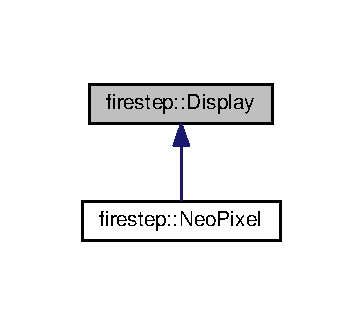
\includegraphics[width=174pt]{classfirestep_1_1_display__inherit__graph}
\end{center}
\end{figure}
\subsection*{Public Member Functions}
\begin{DoxyCompactItemize}
\item 
\hypertarget{classfirestep_1_1_display_ac0e86412cc360a40a30eab70b6a134a9}{virtual void {\bfseries setup} (int pin)}\label{classfirestep_1_1_display_ac0e86412cc360a40a30eab70b6a134a9}

\item 
\hypertarget{classfirestep_1_1_display_a53a9f6a1f5b6a9b092d564177ec17941}{virtual void {\bfseries show} ()}\label{classfirestep_1_1_display_a53a9f6a1f5b6a9b092d564177ec17941}

\item 
\hypertarget{classfirestep_1_1_display_a28fa6497250386b2e0d86604182b60cd}{Display\+Status {\bfseries get\+Status} ()}\label{classfirestep_1_1_display_a28fa6497250386b2e0d86604182b60cd}

\item 
\hypertarget{classfirestep_1_1_display_a101c7faf6934812852889a040c6b912f}{virtual void {\bfseries set\+Status} (Display\+Status status=D\+I\+S\+P\+L\+A\+Y\+\_\+\+W\+A\+I\+T\+\_\+\+I\+D\+L\+E)}\label{classfirestep_1_1_display_a101c7faf6934812852889a040c6b912f}

\item 
\hypertarget{classfirestep_1_1_display_a960ee2cf65689f4da354d3e026020a5a}{uint8\+\_\+t {\bfseries get\+Level} ()}\label{classfirestep_1_1_display_a960ee2cf65689f4da354d3e026020a5a}

\item 
\hypertarget{classfirestep_1_1_display_a8e6a6ac174a4d7f459bf177867d90c27}{virtual void {\bfseries set\+Level} (uint8\+\_\+t level=127)}\label{classfirestep_1_1_display_a8e6a6ac174a4d7f459bf177867d90c27}

\end{DoxyCompactItemize}
\subsection*{Protected Attributes}
\begin{DoxyCompactItemize}
\item 
\hypertarget{classfirestep_1_1_display_acd4ec3ee696e5e44f6cd72b6e7f2b96d}{uint8\+\_\+t {\bfseries status}}\label{classfirestep_1_1_display_acd4ec3ee696e5e44f6cd72b6e7f2b96d}

\item 
\hypertarget{classfirestep_1_1_display_a66292a4fba836ad18de6ab228ddf8b6c}{uint8\+\_\+t {\bfseries level}}\label{classfirestep_1_1_display_a66292a4fba836ad18de6ab228ddf8b6c}

\item 
\hypertarget{classfirestep_1_1_display_ae50b9bb2a8f06e4d1411d1b4543901e4}{uint8\+\_\+t {\bfseries camera\+R}}\label{classfirestep_1_1_display_ae50b9bb2a8f06e4d1411d1b4543901e4}

\item 
\hypertarget{classfirestep_1_1_display_ae0293900c8a1dc8d0a8dd314c02df537}{uint8\+\_\+t {\bfseries camera\+G}}\label{classfirestep_1_1_display_ae0293900c8a1dc8d0a8dd314c02df537}

\item 
\hypertarget{classfirestep_1_1_display_af7d4b636ef027c155c281609a723858f}{uint8\+\_\+t {\bfseries camera\+B}}\label{classfirestep_1_1_display_af7d4b636ef027c155c281609a723858f}

\end{DoxyCompactItemize}
\subsection*{Friends}
\begin{DoxyCompactItemize}
\item 
\hypertarget{classfirestep_1_1_display_a63aca5b4b5947b26b23225194abc1e9c}{class {\bfseries Json\+Controller}}\label{classfirestep_1_1_display_a63aca5b4b5947b26b23225194abc1e9c}

\item 
\hypertarget{classfirestep_1_1_display_a62ce8176f96f110c5d95b6f4cb83bf1d}{class {\bfseries F\+P\+D\+Controller}}\label{classfirestep_1_1_display_a62ce8176f96f110c5d95b6f4cb83bf1d}

\end{DoxyCompactItemize}


The documentation for this class was generated from the following file\+:\begin{DoxyCompactItemize}
\item 
Display.\+h\end{DoxyCompactItemize}

\hypertarget{classfirestep_1_1_f_p_d_calibrate_home}{\section{firestep\+:\+:F\+P\+D\+Calibrate\+Home Class Reference}
\label{classfirestep_1_1_f_p_d_calibrate_home}\index{firestep\+::\+F\+P\+D\+Calibrate\+Home@{firestep\+::\+F\+P\+D\+Calibrate\+Home}}
}


Collaboration diagram for firestep\+:\+:F\+P\+D\+Calibrate\+Home\+:
\nopagebreak
\begin{figure}[H]
\begin{center}
\leavevmode
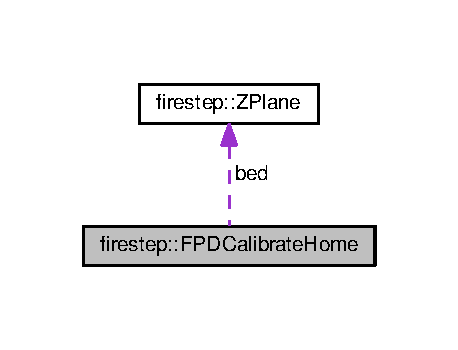
\includegraphics[width=220pt]{classfirestep_1_1_f_p_d_calibrate_home__coll__graph}
\end{center}
\end{figure}
\subsection*{Public Member Functions}
\begin{DoxyCompactItemize}
\item 
\hypertarget{classfirestep_1_1_f_p_d_calibrate_home_a8584d79396fc70f8da0f4be97f0c6d40}{{\bfseries F\+P\+D\+Calibrate\+Home} (\hyperlink{classfirestep_1_1_machine}{Machine} \&machine)}\label{classfirestep_1_1_f_p_d_calibrate_home_a8584d79396fc70f8da0f4be97f0c6d40}

\item 
\hypertarget{classfirestep_1_1_f_p_d_calibrate_home_a37321b6559900418ae63791560aef26a}{Status {\bfseries calibrate} ()}\label{classfirestep_1_1_f_p_d_calibrate_home_a37321b6559900418ae63791560aef26a}

\end{DoxyCompactItemize}
\subsection*{Public Attributes}
\begin{DoxyCompactItemize}
\item 
\hypertarget{classfirestep_1_1_f_p_d_calibrate_home_aa7aa332ee4859b8646ae8cc9010c91b5}{P\+H5\+T\+Y\+P\+E {\bfseries z\+Center}}\label{classfirestep_1_1_f_p_d_calibrate_home_aa7aa332ee4859b8646ae8cc9010c91b5}

\item 
\hypertarget{classfirestep_1_1_f_p_d_calibrate_home_a012c0276dfa8cf8505490253790e5a79}{P\+H5\+T\+Y\+P\+E {\bfseries z\+Rim}}\label{classfirestep_1_1_f_p_d_calibrate_home_a012c0276dfa8cf8505490253790e5a79}

\item 
\hypertarget{classfirestep_1_1_f_p_d_calibrate_home_aabfe8245fdf7e3b80c6f0c4b18db718e}{P\+H5\+T\+Y\+P\+E {\bfseries e\+Theta}}\label{classfirestep_1_1_f_p_d_calibrate_home_aabfe8245fdf7e3b80c6f0c4b18db718e}

\item 
\hypertarget{classfirestep_1_1_f_p_d_calibrate_home_a9105696fde45b04c711c442a6392bd93}{P\+H5\+T\+Y\+P\+E {\bfseries home\+Angle}}\label{classfirestep_1_1_f_p_d_calibrate_home_a9105696fde45b04c711c442a6392bd93}

\item 
\hypertarget{classfirestep_1_1_f_p_d_calibrate_home_a386dd3229fe6b64d25150494048de8bf}{P\+H5\+T\+Y\+P\+E {\bfseries e\+Gear}}\label{classfirestep_1_1_f_p_d_calibrate_home_a386dd3229fe6b64d25150494048de8bf}

\item 
\hypertarget{classfirestep_1_1_f_p_d_calibrate_home_a15d05910bee5d2726f30b9c54f670ef8}{P\+H5\+T\+Y\+P\+E {\bfseries gear\+Ratio}}\label{classfirestep_1_1_f_p_d_calibrate_home_a15d05910bee5d2726f30b9c54f670ef8}

\item 
\hypertarget{classfirestep_1_1_f_p_d_calibrate_home_ae1fc3c7c8d9ab0621b84da772272b4a2}{P\+H5\+T\+Y\+P\+E {\bfseries save\+Weight}}\label{classfirestep_1_1_f_p_d_calibrate_home_ae1fc3c7c8d9ab0621b84da772272b4a2}

\item 
\hypertarget{classfirestep_1_1_f_p_d_calibrate_home_a78abd53e2a1abda12bbe0db21dc6674b}{\hyperlink{classfirestep_1_1_z_plane}{Z\+Plane} {\bfseries bed}}\label{classfirestep_1_1_f_p_d_calibrate_home_a78abd53e2a1abda12bbe0db21dc6674b}

\item 
\hypertarget{classfirestep_1_1_f_p_d_calibrate_home_a7e055a2a1a896bcbbaf7bbe631692cb5}{Calibrate\+Mode {\bfseries mode}}\label{classfirestep_1_1_f_p_d_calibrate_home_a7e055a2a1a896bcbbaf7bbe631692cb5}

\end{DoxyCompactItemize}


The documentation for this class was generated from the following files\+:\begin{DoxyCompactItemize}
\item 
F\+P\+D\+Controller.\+h\item 
F\+P\+D\+Controller.\+cpp\end{DoxyCompactItemize}

\hypertarget{classfirestep_1_1_f_p_d_controller}{\section{firestep\+:\+:F\+P\+D\+Controller Class Reference}
\label{classfirestep_1_1_f_p_d_controller}\index{firestep\+::\+F\+P\+D\+Controller@{firestep\+::\+F\+P\+D\+Controller}}
}


Inheritance diagram for firestep\+:\+:F\+P\+D\+Controller\+:
\nopagebreak
\begin{figure}[H]
\begin{center}
\leavevmode
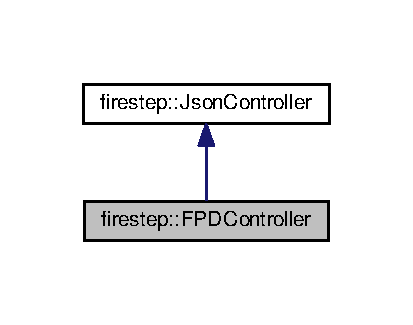
\includegraphics[width=198pt]{classfirestep_1_1_f_p_d_controller__inherit__graph}
\end{center}
\end{figure}


Collaboration diagram for firestep\+:\+:F\+P\+D\+Controller\+:
\nopagebreak
\begin{figure}[H]
\begin{center}
\leavevmode
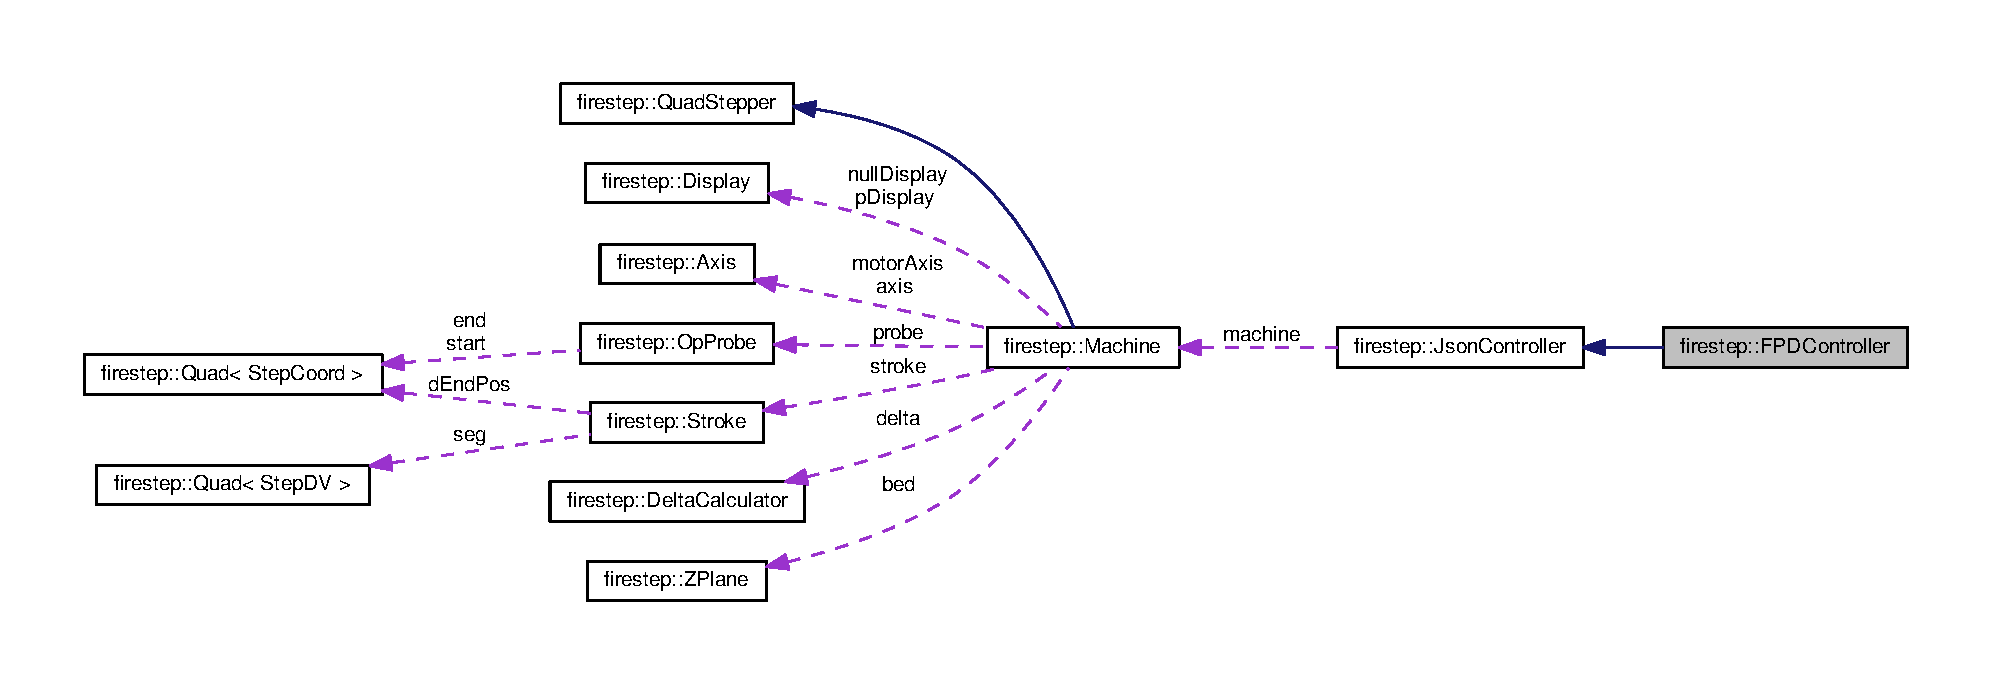
\includegraphics[width=350pt]{classfirestep_1_1_f_p_d_controller__coll__graph}
\end{center}
\end{figure}
\subsection*{Public Member Functions}
\begin{DoxyCompactItemize}
\item 
\hypertarget{classfirestep_1_1_f_p_d_controller_a454af68839decada4629fd40454bf1dc}{{\bfseries F\+P\+D\+Controller} (\hyperlink{classfirestep_1_1_machine}{Machine} \&machine)}\label{classfirestep_1_1_f_p_d_controller_a454af68839decada4629fd40454bf1dc}

\item 
\hypertarget{classfirestep_1_1_f_p_d_controller_acb0505b40ced4c9d25ffc54ed119ec83}{\hyperlink{classfirestep_1_1_x_y_z3_d}{X\+Y\+Z3\+D} {\bfseries get\+X\+Y\+Z3\+D} ()}\label{classfirestep_1_1_f_p_d_controller_acb0505b40ced4c9d25ffc54ed119ec83}

\item 
\hypertarget{classfirestep_1_1_f_p_d_controller_a33cdaa55e8e64a44b05aaf54d506f66f}{virtual const char $\ast$ {\bfseries name} ()}\label{classfirestep_1_1_f_p_d_controller_a33cdaa55e8e64a44b05aaf54d506f66f}

\item 
\hypertarget{classfirestep_1_1_f_p_d_controller_aed5b4cee634eadd56ce6b05a322fa97e}{virtual void {\bfseries on\+Topology\+Changed} ()}\label{classfirestep_1_1_f_p_d_controller_aed5b4cee634eadd56ce6b05a322fa97e}

\end{DoxyCompactItemize}
\subsection*{Protected Member Functions}
\begin{DoxyCompactItemize}
\item 
\hypertarget{classfirestep_1_1_f_p_d_controller_a1b0c93f2e1444bf994b84744450ea5ed}{Status {\bfseries initialize\+Probe\+\_\+\+M\+T\+O\+\_\+\+F\+P\+D} (\hyperlink{classfirestep_1_1_json_command}{Json\+Command} \&jcmd, Json\+Object \&jobj, const char $\ast$key, bool clear)}\label{classfirestep_1_1_f_p_d_controller_a1b0c93f2e1444bf994b84744450ea5ed}

\item 
\hypertarget{classfirestep_1_1_f_p_d_controller_a183bdf8187896f0f348951172b3d6a00}{virtual Status {\bfseries initialize\+Home} (\hyperlink{classfirestep_1_1_json_command}{Json\+Command} \&jcmd, Json\+Object \&jobj, const char $\ast$key, bool clear)}\label{classfirestep_1_1_f_p_d_controller_a183bdf8187896f0f348951172b3d6a00}

\item 
\hypertarget{classfirestep_1_1_f_p_d_controller_aea1fe915de671d24c63457175cbc8b4b}{Status {\bfseries finalize\+Probe\+\_\+\+M\+T\+O\+\_\+\+F\+P\+D} (\hyperlink{classfirestep_1_1_json_command}{Json\+Command} \&jcmd, Json\+Object \&jobj, const char $\ast$key)}\label{classfirestep_1_1_f_p_d_controller_aea1fe915de671d24c63457175cbc8b4b}

\item 
\hypertarget{classfirestep_1_1_f_p_d_controller_a3ec03c9dda441548c65ed322181ea6c8}{Status {\bfseries finalize\+Home} (\hyperlink{classfirestep_1_1_json_command}{Json\+Command} \&jcmd, Json\+Object \&jobj, const char $\ast$key)}\label{classfirestep_1_1_f_p_d_controller_a3ec03c9dda441548c65ed322181ea6c8}

\item 
\hypertarget{classfirestep_1_1_f_p_d_controller_ac63ea83d6a9f94cbb783d55fa6325404}{Status {\bfseries process\+Calibrate\+Core} (\hyperlink{classfirestep_1_1_json_command}{Json\+Command} \&jcmd, Json\+Object \&jobj, const char $\ast$key, \hyperlink{classfirestep_1_1_f_p_d_calibrate_home}{F\+P\+D\+Calibrate\+Home} \&cal, bool output)}\label{classfirestep_1_1_f_p_d_controller_ac63ea83d6a9f94cbb783d55fa6325404}

\item 
\hypertarget{classfirestep_1_1_f_p_d_controller_af320324c335545085a7e4c34128070d9}{virtual Status {\bfseries process\+Mark} (\hyperlink{classfirestep_1_1_json_command}{Json\+Command} \&jcmd, Json\+Object \&jobj, const char $\ast$key)}\label{classfirestep_1_1_f_p_d_controller_af320324c335545085a7e4c34128070d9}

\item 
\hypertarget{classfirestep_1_1_f_p_d_controller_a10e47c83caae217920b8113f5f03b97e}{virtual Status {\bfseries process\+Calibrate} (\hyperlink{classfirestep_1_1_json_command}{Json\+Command} \&jcmd, Json\+Object \&jobj, const char $\ast$keycal)}\label{classfirestep_1_1_f_p_d_controller_a10e47c83caae217920b8113f5f03b97e}

\item 
\hypertarget{classfirestep_1_1_f_p_d_controller_acaffcae5cb21f4caa986097dcbc98d06}{virtual Status {\bfseries process\+Home} (\hyperlink{classfirestep_1_1_json_command}{Json\+Command} \&jcmd, Json\+Object \&jobj, const char $\ast$key)}\label{classfirestep_1_1_f_p_d_controller_acaffcae5cb21f4caa986097dcbc98d06}

\item 
\hypertarget{classfirestep_1_1_f_p_d_controller_acc1a8f014cc048249f8a021dc56df685}{virtual Status {\bfseries process\+Position} (\hyperlink{classfirestep_1_1_json_command}{Json\+Command} \&jcmd, Json\+Object \&jobj, const char $\ast$key)}\label{classfirestep_1_1_f_p_d_controller_acc1a8f014cc048249f8a021dc56df685}

\item 
\hypertarget{classfirestep_1_1_f_p_d_controller_a5569d32e75cc338582233f7306c9f67e}{virtual Status {\bfseries process\+Probe} (\hyperlink{classfirestep_1_1_json_command}{Json\+Command} \&jcmd, Json\+Object \&jobj, const char $\ast$key)}\label{classfirestep_1_1_f_p_d_controller_a5569d32e75cc338582233f7306c9f67e}

\item 
\hypertarget{classfirestep_1_1_f_p_d_controller_a5d0ffeb2eb45d27e05cba3b92bd4c41b}{virtual Status {\bfseries process\+Dimension} (\hyperlink{classfirestep_1_1_json_command}{Json\+Command} \&jcmd, Json\+Object \&jobj, const char $\ast$key)}\label{classfirestep_1_1_f_p_d_controller_a5d0ffeb2eb45d27e05cba3b92bd4c41b}

\item 
\hypertarget{classfirestep_1_1_f_p_d_controller_ab13174b90ccd66e022b0d11f79fe896d}{virtual Status {\bfseries process\+Move} (\hyperlink{classfirestep_1_1_json_command}{Json\+Command} \&jcmd, Json\+Object \&jobj, const char $\ast$key)}\label{classfirestep_1_1_f_p_d_controller_ab13174b90ccd66e022b0d11f79fe896d}

\end{DoxyCompactItemize}
\subsection*{Additional Inherited Members}


The documentation for this class was generated from the following files\+:\begin{DoxyCompactItemize}
\item 
F\+P\+D\+Controller.\+h\item 
F\+P\+D\+Controller.\+cpp\end{DoxyCompactItemize}

\hypertarget{class_f_p_d_move_to}{\section{F\+P\+D\+Move\+To Class Reference}
\label{class_f_p_d_move_to}\index{F\+P\+D\+Move\+To@{F\+P\+D\+Move\+To}}
}
\subsection*{Public Member Functions}
\begin{DoxyCompactItemize}
\item 
\hypertarget{class_f_p_d_move_to_a686b5198381fa8e19e5c9956a6575124}{{\bfseries F\+P\+D\+Move\+To} (\hyperlink{classfirestep_1_1_f_p_d_controller}{F\+P\+D\+Controller} \&controller, \hyperlink{classfirestep_1_1_machine}{Machine} \&machine)}\label{class_f_p_d_move_to_a686b5198381fa8e19e5c9956a6575124}

\item 
\hypertarget{class_f_p_d_move_to_a4b30a96bbd91a4a5315d7bb641b353b5}{Status {\bfseries process} (\hyperlink{classfirestep_1_1_json_command}{Json\+Command} \&jcmd, Json\+Object \&jobj, const char $\ast$key)}\label{class_f_p_d_move_to_a4b30a96bbd91a4a5315d7bb641b353b5}

\end{DoxyCompactItemize}


The documentation for this class was generated from the following file\+:\begin{DoxyCompactItemize}
\item 
F\+P\+D\+Controller.\+cpp\end{DoxyCompactItemize}

\hypertarget{classfirestep_1_1_json_command}{\section{firestep\+:\+:Json\+Command Class Reference}
\label{classfirestep_1_1_json_command}\index{firestep\+::\+Json\+Command@{firestep\+::\+Json\+Command}}
}
\subsection*{Public Member Functions}
\begin{DoxyCompactItemize}
\item 
\hypertarget{classfirestep_1_1_json_command_ac83671bb231c397f90a69d80a661b22b}{void {\bfseries clear} ()}\label{classfirestep_1_1_json_command_ac83671bb231c397f90a69d80a661b22b}

\item 
\hypertarget{classfirestep_1_1_json_command_ae255c66670150f7e2f3f00a1c613e7bb}{Json\+Variant \& {\bfseries request\+Root} ()}\label{classfirestep_1_1_json_command_ae255c66670150f7e2f3f00a1c613e7bb}

\item 
\hypertarget{classfirestep_1_1_json_command_afe7d7d544df5026b32813aeec691a746}{Json\+Object \& {\bfseries response} ()}\label{classfirestep_1_1_json_command_afe7d7d544df5026b32813aeec691a746}

\item 
Status \hyperlink{classfirestep_1_1_json_command_a569a3db08111c18c7a56d18f507c26b3}{parse} (const char $\ast$json\+In, Status status=S\+T\+A\+T\+U\+S\+\_\+\+W\+A\+I\+T\+\_\+\+I\+D\+L\+E)
\item 
\hypertarget{classfirestep_1_1_json_command_a58e091d27a40ac612cf3627d52f1ac53}{bool {\bfseries is\+Valid} ()}\label{classfirestep_1_1_json_command_a58e091d27a40ac612cf3627d52f1ac53}

\item 
\hypertarget{classfirestep_1_1_json_command_aa2f8350ff5c70fab26adea09590dda71}{Status {\bfseries get\+Status} ()}\label{classfirestep_1_1_json_command_aa2f8350ff5c70fab26adea09590dda71}

\item 
\hypertarget{classfirestep_1_1_json_command_a1e1211ff3366029bcbc8cc3a880c17f2}{void {\bfseries set\+Ticks} ()}\label{classfirestep_1_1_json_command_a1e1211ff3366029bcbc8cc3a880c17f2}

\item 
\hypertarget{classfirestep_1_1_json_command_ad609d3cde9564aabf3a7319fdd8732ec}{void {\bfseries set\+Status} (Status status)}\label{classfirestep_1_1_json_command_ad609d3cde9564aabf3a7319fdd8732ec}

\item 
\hypertarget{classfirestep_1_1_json_command_a50064a31b57d68d2aa26408ad19e132d}{const char $\ast$ {\bfseries get\+Error} ()}\label{classfirestep_1_1_json_command_a50064a31b57d68d2aa26408ad19e132d}

\item 
\hypertarget{classfirestep_1_1_json_command_a017a69509a155996f74ac9ab14011fb4}{Status {\bfseries set\+Error} (Status status, const char $\ast$err)}\label{classfirestep_1_1_json_command_a017a69509a155996f74ac9ab14011fb4}

\item 
\hypertarget{classfirestep_1_1_json_command_a735a49fec2c5971eb1cb1931868498ff}{size\+\_\+t {\bfseries request\+Available} ()}\label{classfirestep_1_1_json_command_a735a49fec2c5971eb1cb1931868498ff}

\item 
\hypertarget{classfirestep_1_1_json_command_a9f0c38e162c823239de9c6b9f66d8b68}{size\+\_\+t {\bfseries response\+Available} ()}\label{classfirestep_1_1_json_command_a9f0c38e162c823239de9c6b9f66d8b68}

\item 
\hypertarget{classfirestep_1_1_json_command_a5d3bdb1c9fa849772e8fefefdf0b6cb4}{size\+\_\+t {\bfseries request\+Capacity} ()}\label{classfirestep_1_1_json_command_a5d3bdb1c9fa849772e8fefefdf0b6cb4}

\item 
\hypertarget{classfirestep_1_1_json_command_a551c8f29c2cee51a8b63e0677e370b24}{size\+\_\+t {\bfseries response\+Capacity} ()}\label{classfirestep_1_1_json_command_a551c8f29c2cee51a8b63e0677e370b24}

\item 
\hypertarget{classfirestep_1_1_json_command_a06e0d10496ac3f0901b820aca5592f62}{void {\bfseries response\+Clear} ()}\label{classfirestep_1_1_json_command_a06e0d10496ac3f0901b820aca5592f62}

\item 
\hypertarget{classfirestep_1_1_json_command_a9c237e80cea28bbf85138041e08f6640}{char $\ast$ {\bfseries allocate} (size\+\_\+t length)}\label{classfirestep_1_1_json_command_a9c237e80cea28bbf85138041e08f6640}

\item 
\hypertarget{classfirestep_1_1_json_command_a238279d60501a357ca4b48e798838378}{void {\bfseries add\+Query\+Attr} (Json\+Object \&node, const char $\ast$key)}\label{classfirestep_1_1_json_command_a238279d60501a357ca4b48e798838378}

\end{DoxyCompactItemize}
\subsection*{Public Attributes}
\begin{DoxyCompactItemize}
\item 
\hypertarget{classfirestep_1_1_json_command_ac15733c34e8b5c9ae30ed66d361c9d95}{Json\+Variant {\bfseries j\+Response\+Root}}\label{classfirestep_1_1_json_command_ac15733c34e8b5c9ae30ed66d361c9d95}

\item 
\hypertarget{classfirestep_1_1_json_command_a9174a0b92995dc7b01d9f06bfc6ffe7c}{int8\+\_\+t {\bfseries cmd\+Index}}\label{classfirestep_1_1_json_command_a9174a0b92995dc7b01d9f06bfc6ffe7c}

\end{DoxyCompactItemize}
\subsection*{Friends}
\begin{DoxyCompactItemize}
\item 
\hypertarget{classfirestep_1_1_json_command_a63aca5b4b5947b26b23225194abc1e9c}{class {\bfseries Json\+Controller}}\label{classfirestep_1_1_json_command_a63aca5b4b5947b26b23225194abc1e9c}

\item 
\hypertarget{classfirestep_1_1_json_command_a62ce8176f96f110c5d95b6f4cb83bf1d}{class {\bfseries F\+P\+D\+Controller}}\label{classfirestep_1_1_json_command_a62ce8176f96f110c5d95b6f4cb83bf1d}

\end{DoxyCompactItemize}


\subsection{Member Function Documentation}
\hypertarget{classfirestep_1_1_json_command_a569a3db08111c18c7a56d18f507c26b3}{\index{firestep\+::\+Json\+Command@{firestep\+::\+Json\+Command}!parse@{parse}}
\index{parse@{parse}!firestep\+::\+Json\+Command@{firestep\+::\+Json\+Command}}
\subsubsection[{parse}]{\setlength{\rightskip}{0pt plus 5cm}Status Json\+Command\+::parse (
\begin{DoxyParamCaption}
\item[{const char $\ast$}]{json\+In, }
\item[{Status}]{status\+In = {\ttfamily STATUS\+\_\+WAIT\+\_\+IDLE}}
\end{DoxyParamCaption}
)}}\label{classfirestep_1_1_json_command_a569a3db08111c18c7a56d18f507c26b3}
Parse the J\+S\+O\+N provided or a J\+S\+O\+N line read from Serial Return true if parsing is complete. Check is\+Valid() and get\+Status() for parsing status. 

The documentation for this class was generated from the following files\+:\begin{DoxyCompactItemize}
\item 
Json\+Command.\+h\item 
Json\+Command.\+cpp\end{DoxyCompactItemize}

\hypertarget{classfirestep_1_1_json_controller}{\section{firestep\+:\+:Json\+Controller Class Reference}
\label{classfirestep_1_1_json_controller}\index{firestep\+::\+Json\+Controller@{firestep\+::\+Json\+Controller}}
}


Inheritance diagram for firestep\+:\+:Json\+Controller\+:
\nopagebreak
\begin{figure}[H]
\begin{center}
\leavevmode
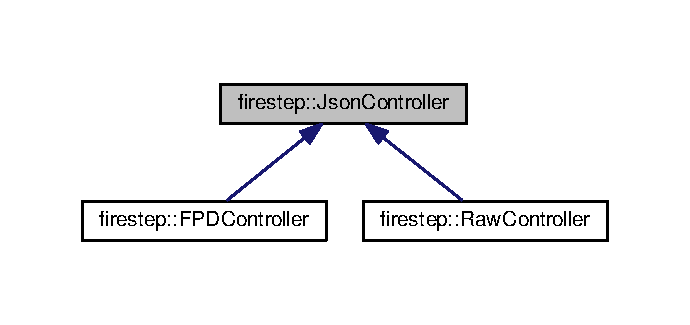
\includegraphics[width=331pt]{classfirestep_1_1_json_controller__inherit__graph}
\end{center}
\end{figure}


Collaboration diagram for firestep\+:\+:Json\+Controller\+:
\nopagebreak
\begin{figure}[H]
\begin{center}
\leavevmode
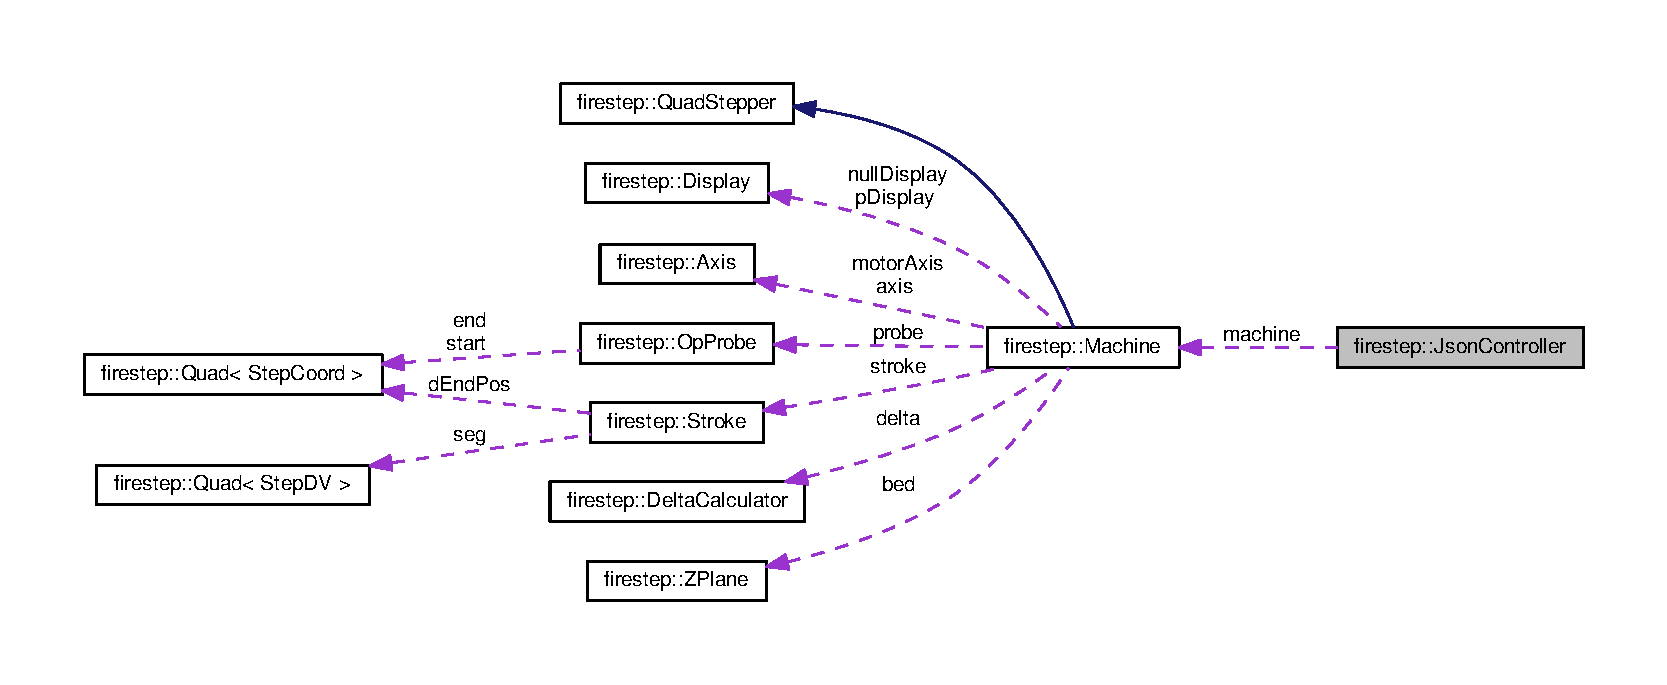
\includegraphics[width=350pt]{classfirestep_1_1_json_controller__coll__graph}
\end{center}
\end{figure}
\subsection*{Public Member Functions}
\begin{DoxyCompactItemize}
\item 
\hypertarget{classfirestep_1_1_json_controller_aa99c033aaa8cd12b4ca02eb095309cba}{{\bfseries Json\+Controller} (\hyperlink{classfirestep_1_1_machine}{Machine} \&machine)}\label{classfirestep_1_1_json_controller_aa99c033aaa8cd12b4ca02eb095309cba}

\item 
\hypertarget{classfirestep_1_1_json_controller_ab896ca30795d53a2b1dbb4f6512bcab4}{void {\bfseries send\+Response} (\hyperlink{classfirestep_1_1_json_command}{Json\+Command} \&jcmd, Status status, bool final=true)}\label{classfirestep_1_1_json_controller_ab896ca30795d53a2b1dbb4f6512bcab4}

\item 
\hypertarget{classfirestep_1_1_json_controller_a81ace494431cde7ddeaf6b2004f389b5}{Status {\bfseries process\+Obj} (\hyperlink{classfirestep_1_1_json_command}{Json\+Command} \&jcmd, Json\+Object \&jobj)}\label{classfirestep_1_1_json_controller_a81ace494431cde7ddeaf6b2004f389b5}

\item 
\hypertarget{classfirestep_1_1_json_controller_ae07fb11355da2ca9b32623ed1265718a}{\hyperlink{classfirestep_1_1_json_controller}{Json\+Controller} \& {\bfseries operator=} (\hyperlink{classfirestep_1_1_json_controller}{Json\+Controller} \&that)}\label{classfirestep_1_1_json_controller_ae07fb11355da2ca9b32623ed1265718a}

\item 
\hypertarget{classfirestep_1_1_json_controller_a0a117c0ce47f5c0304b5aa0153077ee1}{Status {\bfseries cancel} (\hyperlink{classfirestep_1_1_json_command}{Json\+Command} \&jcmd, Status cause)}\label{classfirestep_1_1_json_controller_a0a117c0ce47f5c0304b5aa0153077ee1}

\item 
\hypertarget{classfirestep_1_1_json_controller_a51e5351248ad28d3c40c9befd49d879a}{virtual void {\bfseries on\+Topology\+Changed} ()}\label{classfirestep_1_1_json_controller_a51e5351248ad28d3c40c9befd49d879a}

\item 
\hypertarget{classfirestep_1_1_json_controller_a86a2069cce59a7465db39587a912025f}{virtual const char $\ast$ {\bfseries name} ()=0}\label{classfirestep_1_1_json_controller_a86a2069cce59a7465db39587a912025f}

\end{DoxyCompactItemize}
\subsection*{Protected Member Functions}
\begin{DoxyCompactItemize}
\item 
\hypertarget{classfirestep_1_1_json_controller_af7d36ec60276471ee6b57d857778aa28}{Axis\+Index {\bfseries axis\+Of} (char c)}\label{classfirestep_1_1_json_controller_af7d36ec60276471ee6b57d857778aa28}

\item 
\hypertarget{classfirestep_1_1_json_controller_a5c1043d5d57d4e1d9c9a77f35d0aeca6}{virtual Status {\bfseries initialize\+Home} (\hyperlink{classfirestep_1_1_json_command}{Json\+Command} \&jcmd, Json\+Object \&jobj, const char $\ast$key, bool clear)=0}\label{classfirestep_1_1_json_controller_a5c1043d5d57d4e1d9c9a77f35d0aeca6}

\item 
\hypertarget{classfirestep_1_1_json_controller_a239c567f49d1b693fcdc5ee8399bceed}{virtual Status {\bfseries initialize\+Stroke} (\hyperlink{classfirestep_1_1_json_command}{Json\+Command} \&jcmd, Json\+Object \&stroke)}\label{classfirestep_1_1_json_controller_a239c567f49d1b693fcdc5ee8399bceed}

\item 
\hypertarget{classfirestep_1_1_json_controller_a55dccd5b44896199a0d29d5e8e9e6493}{virtual Status {\bfseries process\+Axis} (\hyperlink{classfirestep_1_1_json_command}{Json\+Command} \&jcmd, Json\+Object \&jobj, const char $\ast$key, char group)}\label{classfirestep_1_1_json_controller_a55dccd5b44896199a0d29d5e8e9e6493}

\item 
\hypertarget{classfirestep_1_1_json_controller_a98972901221d243c92e1344adab52d29}{virtual Status {\bfseries process\+Calibrate} (\hyperlink{classfirestep_1_1_json_command}{Json\+Command} \&jcmd, Json\+Object \&jobj, const char $\ast$key)}\label{classfirestep_1_1_json_controller_a98972901221d243c92e1344adab52d29}

\item 
\hypertarget{classfirestep_1_1_json_controller_aa64294812025ca87c3e3550b4a481720}{virtual Status {\bfseries process\+Debug} (\hyperlink{classfirestep_1_1_json_command}{Json\+Command} \&jcmd, Json\+Object \&jobj, const char $\ast$key)}\label{classfirestep_1_1_json_controller_aa64294812025ca87c3e3550b4a481720}

\item 
\hypertarget{classfirestep_1_1_json_controller_a8651e8746ec0178e6755bb33ccace7e9}{virtual Status {\bfseries process\+Dimension} (\hyperlink{classfirestep_1_1_json_command}{Json\+Command} \&jcmd, Json\+Object \&jobj, const char $\ast$key)=0}\label{classfirestep_1_1_json_controller_a8651e8746ec0178e6755bb33ccace7e9}

\item 
\hypertarget{classfirestep_1_1_json_controller_aad0012ee127086fc26f24bb16474a799}{virtual Status {\bfseries process\+Display} (\hyperlink{classfirestep_1_1_json_command}{Json\+Command} \&jcmd, Json\+Object \&jobj, const char $\ast$key)}\label{classfirestep_1_1_json_controller_aad0012ee127086fc26f24bb16474a799}

\item 
\hypertarget{classfirestep_1_1_json_controller_a3b17dbe58969ed24ce43de28cc2ec1f4}{virtual Status {\bfseries process\+E\+E\+P\+R\+O\+M} (\hyperlink{classfirestep_1_1_json_command}{Json\+Command} \&jcmd, Json\+Object \&jobj, const char $\ast$key)}\label{classfirestep_1_1_json_controller_a3b17dbe58969ed24ce43de28cc2ec1f4}

\item 
\hypertarget{classfirestep_1_1_json_controller_ac53a572f0e97b3fade095091ecbec47d}{virtual Status {\bfseries process\+E\+E\+P\+R\+O\+M\+Value} (\hyperlink{classfirestep_1_1_json_command}{Json\+Command} \&jcmd, Json\+Object \&jobj, const char $\ast$key, const char $\ast$addr)}\label{classfirestep_1_1_json_controller_ac53a572f0e97b3fade095091ecbec47d}

\item 
\hypertarget{classfirestep_1_1_json_controller_a193d58f79d46163316dc6520172873be}{virtual Status {\bfseries process\+Home} (\hyperlink{classfirestep_1_1_json_command}{Json\+Command} \&jcmd, Json\+Object \&jobj, const char $\ast$key)=0}\label{classfirestep_1_1_json_controller_a193d58f79d46163316dc6520172873be}

\item 
\hypertarget{classfirestep_1_1_json_controller_a1a065c8490127a1722d4746d80fb7ddf}{virtual Status {\bfseries process\+I\+O} (\hyperlink{classfirestep_1_1_json_command}{Json\+Command} \&jcmd, Json\+Object \&jobj, const char $\ast$key, bool pull\+Up=false)}\label{classfirestep_1_1_json_controller_a1a065c8490127a1722d4746d80fb7ddf}

\item 
\hypertarget{classfirestep_1_1_json_controller_af6211759689e5f895a584b5d1f9b15ef}{virtual Status {\bfseries process\+I\+O\+Pin} (\hyperlink{classfirestep_1_1_json_command}{Json\+Command} \&jcmd, Json\+Object \&jobj, const char $\ast$key, bool pull\+Up)}\label{classfirestep_1_1_json_controller_af6211759689e5f895a584b5d1f9b15ef}

\item 
\hypertarget{classfirestep_1_1_json_controller_a6ebf943b4d72b23bc691427993711e63}{virtual Status {\bfseries process\+Mark} (\hyperlink{classfirestep_1_1_json_command}{Json\+Command} \&jcmd, Json\+Object \&jobj, const char $\ast$key)}\label{classfirestep_1_1_json_controller_a6ebf943b4d72b23bc691427993711e63}

\item 
\hypertarget{classfirestep_1_1_json_controller_a4b24a4eb2b560f67a2b05cfc6de0ffb8}{virtual Status {\bfseries process\+Motor} (\hyperlink{classfirestep_1_1_json_command}{Json\+Command} \&jcmd, Json\+Object \&jobj, const char $\ast$key, char group)}\label{classfirestep_1_1_json_controller_a4b24a4eb2b560f67a2b05cfc6de0ffb8}

\item 
\hypertarget{classfirestep_1_1_json_controller_aba71d8b07eb77cd80b0bb96d2a7d4c67}{virtual Status {\bfseries process\+Move} (\hyperlink{classfirestep_1_1_json_command}{Json\+Command} \&jcmd, Json\+Object \&jobj, const char $\ast$key)=0}\label{classfirestep_1_1_json_controller_aba71d8b07eb77cd80b0bb96d2a7d4c67}

\item 
\hypertarget{classfirestep_1_1_json_controller_ac3fd3ce1124de17ae8ff272a2dfaa2a9}{virtual Status {\bfseries process\+Pin} (Json\+Object \&jobj, const char $\ast$key, Pin\+Type \&pin, int16\+\_\+t mode, int16\+\_\+t value=L\+O\+W)}\label{classfirestep_1_1_json_controller_ac3fd3ce1124de17ae8ff272a2dfaa2a9}

\item 
\hypertarget{classfirestep_1_1_json_controller_ac0fc6e48c99ee31bf82b1915b2dade75}{virtual Status {\bfseries process\+Position} (\hyperlink{classfirestep_1_1_json_command}{Json\+Command} \&jcmd, Json\+Object \&jobj, const char $\ast$key)=0}\label{classfirestep_1_1_json_controller_ac0fc6e48c99ee31bf82b1915b2dade75}

\item 
\hypertarget{classfirestep_1_1_json_controller_adf94382ea3d8cbd30ae8b10980b4bbb6}{virtual Status {\bfseries process\+Probe} (\hyperlink{classfirestep_1_1_json_command}{Json\+Command} \&jcmd, Json\+Object \&jobj, const char $\ast$key)=0}\label{classfirestep_1_1_json_controller_adf94382ea3d8cbd30ae8b10980b4bbb6}

\item 
\hypertarget{classfirestep_1_1_json_controller_ab8fa4e528e77669b5fb9fbd8078560de}{virtual Status {\bfseries process\+Probe\+Data} (\hyperlink{classfirestep_1_1_json_command}{Json\+Command} \&jcmd, Json\+Object \&jobj, const char $\ast$key)}\label{classfirestep_1_1_json_controller_ab8fa4e528e77669b5fb9fbd8078560de}

\item 
\hypertarget{classfirestep_1_1_json_controller_af184788b4e2fee1e820b8c2dd180e5c7}{virtual Status {\bfseries process\+Program} (\hyperlink{classfirestep_1_1_json_command}{Json\+Command} \&jcmd, Json\+Object \&jobj, const char $\ast$key)}\label{classfirestep_1_1_json_controller_af184788b4e2fee1e820b8c2dd180e5c7}

\item 
\hypertarget{classfirestep_1_1_json_controller_a4a696fb7b779e5223224224d99de1c51}{virtual Status {\bfseries process\+Stroke} (\hyperlink{classfirestep_1_1_json_command}{Json\+Command} \&jcmd, Json\+Object \&jobj, const char $\ast$key)}\label{classfirestep_1_1_json_controller_a4a696fb7b779e5223224224d99de1c51}

\item 
\hypertarget{classfirestep_1_1_json_controller_a37b35033be6e43d4681402fe5771a6cd}{virtual Status {\bfseries process\+Sys} (\hyperlink{classfirestep_1_1_json_command}{Json\+Command} \&jcmd, Json\+Object \&jobj, const char $\ast$key)}\label{classfirestep_1_1_json_controller_a37b35033be6e43d4681402fe5771a6cd}

\item 
\hypertarget{classfirestep_1_1_json_controller_a1dadb5a54b51ae0d6987a2c13eec3b1a}{virtual Status {\bfseries process\+Test} (\hyperlink{classfirestep_1_1_json_command}{Json\+Command} \&jcmd, Json\+Object \&jobj, const char $\ast$key)}\label{classfirestep_1_1_json_controller_a1dadb5a54b51ae0d6987a2c13eec3b1a}

\item 
\hypertarget{classfirestep_1_1_json_controller_a5719064f51231ec7352716e80154272c}{virtual Status {\bfseries process\+Tmc} (\hyperlink{classfirestep_1_1_json_command}{Json\+Command} \&jcmd, Json\+Object \&jobj, const char $\ast$key)}\label{classfirestep_1_1_json_controller_a5719064f51231ec7352716e80154272c}

\item 
\hypertarget{classfirestep_1_1_json_controller_a91863b815502ebe3a64c58272a995a33}{virtual Status {\bfseries process\+\_\+id} (\hyperlink{classfirestep_1_1_json_command}{Json\+Command} \&jcmd, Json\+Object \&jobj, const char $\ast$key)}\label{classfirestep_1_1_json_controller_a91863b815502ebe3a64c58272a995a33}

\item 
\hypertarget{classfirestep_1_1_json_controller_a563707aedbfe5720942326aa890cb342}{virtual Status {\bfseries traverse\+Stroke} (\hyperlink{classfirestep_1_1_json_command}{Json\+Command} \&jcmd, Json\+Object \&stroke)}\label{classfirestep_1_1_json_controller_a563707aedbfe5720942326aa890cb342}

\end{DoxyCompactItemize}
\subsection*{Protected Attributes}
\begin{DoxyCompactItemize}
\item 
\hypertarget{classfirestep_1_1_json_controller_aba224062a07e57d7afaaca88f4f48370}{\hyperlink{classfirestep_1_1_machine}{Machine} \& {\bfseries machine}}\label{classfirestep_1_1_json_controller_aba224062a07e57d7afaaca88f4f48370}

\end{DoxyCompactItemize}


The documentation for this class was generated from the following files\+:\begin{DoxyCompactItemize}
\item 
Json\+Controller.\+h\item 
Json\+Controller.\+cpp\end{DoxyCompactItemize}

\hypertarget{classfirestep_1_1_machine}{\section{firestep\+:\+:Machine Class Reference}
\label{classfirestep_1_1_machine}\index{firestep\+::\+Machine@{firestep\+::\+Machine}}
}


Inheritance diagram for firestep\+:\+:Machine\+:\nopagebreak
\begin{figure}[H]
\begin{center}
\leavevmode
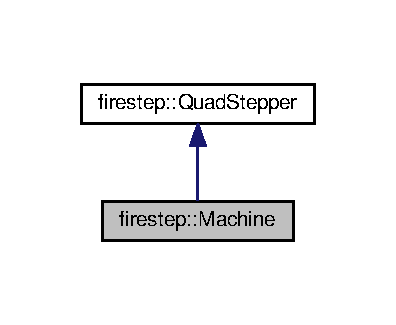
\includegraphics[width=190pt]{classfirestep_1_1_machine__inherit__graph}
\end{center}
\end{figure}


Collaboration diagram for firestep\+:\+:Machine\+:
\nopagebreak
\begin{figure}[H]
\begin{center}
\leavevmode
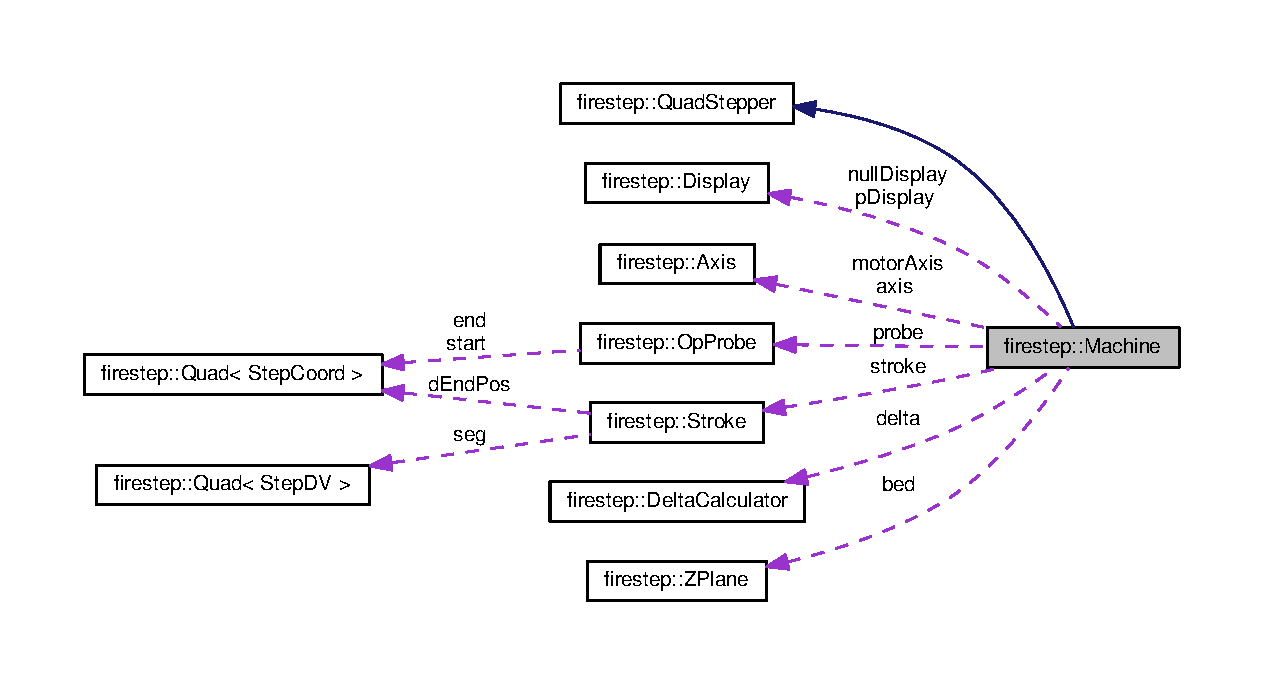
\includegraphics[width=350pt]{classfirestep_1_1_machine__coll__graph}
\end{center}
\end{figure}
\subsection*{Public Member Functions}
\begin{DoxyCompactItemize}
\item 
\hypertarget{classfirestep_1_1_machine_a4b0eee05edc1cdd59749b27099a8fdee}{void {\bfseries setup} (Pin\+Config cfg)}\label{classfirestep_1_1_machine_a4b0eee05edc1cdd59749b27099a8fdee}

\item 
\hypertarget{classfirestep_1_1_machine_a60063b1edb804c45b0b10babf539582a}{int32\+\_\+t {\bfseries hash} ()}\label{classfirestep_1_1_machine_a60063b1edb804c45b0b10babf539582a}

\item 
virtual Status \hyperlink{classfirestep_1_1_machine_a581b2333ca877f4ea4c020eaaaf485f3}{step} (const \hyperlink{classfirestep_1_1_quad}{Quad}$<$ Step\+D\+V $>$ \&\hyperlink{classfirestep_1_1_machine_a01596c1eb82ee853417f77404317c4ed}{pulse})
\item 
\hypertarget{classfirestep_1_1_machine_a97d0850669e905e5adca4933f649342d}{bool {\bfseries is\+Core\+Pin} (int16\+\_\+t pin)}\label{classfirestep_1_1_machine_a97d0850669e905e5adca4933f649342d}

\item 
\hypertarget{classfirestep_1_1_machine_a3c5a08b9a838939ab4d58b474dd53fc4}{bool {\bfseries is\+At\+Limit} (Pin\+Type pin)}\label{classfirestep_1_1_machine_a3c5a08b9a838939ab4d58b474dd53fc4}

\item 
\hypertarget{classfirestep_1_1_machine_a87a7f34fb93980c64fa04f36ff86eae3}{int8\+\_\+t {\bfseries pulse\+Pin} (int16\+\_\+t pin\+Step, int8\+\_\+t n)}\label{classfirestep_1_1_machine_a87a7f34fb93980c64fa04f36ff86eae3}

\item 
\hypertarget{classfirestep_1_1_machine_ac40d24bb9d52ecac4c0370221c9364ff}{Status {\bfseries step\+Fast} (\hyperlink{classfirestep_1_1_quad}{Quad}$<$ Step\+D\+V $>$ \&\hyperlink{classfirestep_1_1_machine_a01596c1eb82ee853417f77404317c4ed}{pulse})}\label{classfirestep_1_1_machine_ac40d24bb9d52ecac4c0370221c9364ff}

\item 
virtual Status \hyperlink{classfirestep_1_1_machine_ad3cfb55e4071b4d20855175beb21ed6a}{step\+Direction} (const \hyperlink{classfirestep_1_1_quad}{Quad}$<$ Step\+D\+V $>$ \&\hyperlink{classfirestep_1_1_machine_a01596c1eb82ee853417f77404317c4ed}{pulse})
\item 
Status \hyperlink{classfirestep_1_1_machine_a01596c1eb82ee853417f77404317c4ed}{pulse} (\hyperlink{classfirestep_1_1_quad}{Quad}$<$ Step\+Coord $>$ \&pulses)
\item 
\hypertarget{classfirestep_1_1_machine_a78860fbc2ac4433bc2f690db1019d8b9}{void {\bfseries set\+Pin} (Pin\+Type \&pin\+Dst, Pin\+Type pin\+Src, int16\+\_\+t mode, int16\+\_\+t value=L\+O\+W)}\label{classfirestep_1_1_machine_a78860fbc2ac4433bc2f690db1019d8b9}

\item 
\hyperlink{classfirestep_1_1_quad}{Quad}$<$ Step\+Coord $>$ \hyperlink{classfirestep_1_1_machine_abb9ab1d2cc47dca81eed644f0cc73a05}{get\+Motor\+Position} ()
\item 
void \hyperlink{classfirestep_1_1_machine_a6a92108622bf3dd555c32ffbea7b0f7a}{set\+Motor\+Position} (const \hyperlink{classfirestep_1_1_quad}{Quad}$<$ Step\+Coord $>$ \&position)
\item 
\hypertarget{classfirestep_1_1_machine_a28830b2f79fac4a0432edaf6b9a27101}{virtual Status {\bfseries home} (Status status)}\label{classfirestep_1_1_machine_a28830b2f79fac4a0432edaf6b9a27101}

\item 
\hypertarget{classfirestep_1_1_machine_a5dd121622a9f9284e51bfa0c1428c792}{virtual Status {\bfseries probe} (Status status, Delay\+Mics delay=-\/1)}\label{classfirestep_1_1_machine_a5dd121622a9f9284e51bfa0c1428c792}

\item 
\hypertarget{classfirestep_1_1_machine_a63a5c312904451636ec96ec143d3f1fd}{Status {\bfseries set\+Axis\+Index} (Motor\+Index i\+Motor, Axis\+Index i\+Axis)}\label{classfirestep_1_1_machine_a63a5c312904451636ec96ec143d3f1fd}

\item 
\hypertarget{classfirestep_1_1_machine_a48b2fc0944ac40ec8ecd06d6d877b682}{Axis\+Index {\bfseries get\+Axis\+Index} (Motor\+Index i\+Motor)}\label{classfirestep_1_1_machine_a48b2fc0944ac40ec8ecd06d6d877b682}

\item 
\hypertarget{classfirestep_1_1_machine_a22d975f5164145e181bdd1a879816082}{\hyperlink{classfirestep_1_1_axis}{Axis} \& {\bfseries get\+Motor\+Axis} (Motor\+Index i\+Motor)}\label{classfirestep_1_1_machine_a22d975f5164145e181bdd1a879816082}

\item 
\hypertarget{classfirestep_1_1_machine_a62bdc431a0fe53a0da676f97da35f744}{Motor\+Index {\bfseries motor\+Of\+Name} (const char $\ast$name)}\label{classfirestep_1_1_machine_a62bdc431a0fe53a0da676f97da35f744}

\item 
\hypertarget{classfirestep_1_1_machine_a5288737d66d3117e4593af57831d7e57}{Axis\+Index {\bfseries axis\+Of\+Name} (const char $\ast$name)}\label{classfirestep_1_1_machine_a5288737d66d3117e4593af57831d7e57}

\item 
\hypertarget{classfirestep_1_1_machine_ad38b0d760dd6eda13d06876192c6418e}{Status {\bfseries set\+Pin\+Config} (Pin\+Config pc)}\label{classfirestep_1_1_machine_ad38b0d760dd6eda13d06876192c6418e}

\item 
\hypertarget{classfirestep_1_1_machine_a773c07a6e2d06a51d836b996c6c45a5a}{Pin\+Config {\bfseries get\+Pin\+Config} ()}\label{classfirestep_1_1_machine_a773c07a6e2d06a51d836b996c6c45a5a}

\item 
\hypertarget{classfirestep_1_1_machine_a44d29a2c0cd0c9469d3eb4d4d7ea1cd9}{char $\ast$ {\bfseries save\+Sys\+Config} (char $\ast$out, size\+\_\+t max\+Len)}\label{classfirestep_1_1_machine_a44d29a2c0cd0c9469d3eb4d4d7ea1cd9}

\item 
\hypertarget{classfirestep_1_1_machine_a07825c242d26746ac674ec433ee1461a}{char $\ast$ {\bfseries save\+Dim\+Config} (char $\ast$out, size\+\_\+t max\+Len)}\label{classfirestep_1_1_machine_a07825c242d26746ac674ec433ee1461a}

\item 
\hypertarget{classfirestep_1_1_machine_afdb1abb94c1d775d317b83aefc355f37}{Status {\bfseries idle} (Status status)}\label{classfirestep_1_1_machine_afdb1abb94c1d775d317b83aefc355f37}

\item 
\hypertarget{classfirestep_1_1_machine_a5c6d3c34db64ebbb576522e37ea2703e}{Status {\bfseries sync} (Status status)}\label{classfirestep_1_1_machine_a5c6d3c34db64ebbb576522e37ea2703e}

\item 
\hypertarget{classfirestep_1_1_machine_a8d98e99157176991d51f752913ccb448}{void {\bfseries enable\+E\+E\+User} (bool enable)}\label{classfirestep_1_1_machine_a8d98e99157176991d51f752913ccb448}

\item 
\hypertarget{classfirestep_1_1_machine_a5a7088ff22ea433073b82551523dae3d}{bool {\bfseries is\+E\+E\+User\+Enabled} ()}\label{classfirestep_1_1_machine_a5a7088ff22ea433073b82551523dae3d}

\item 
\hypertarget{classfirestep_1_1_machine_affe2e3dbc49b0c0d970258694ecadf1a}{void {\bfseries load\+Delta\+Calculator} ()}\label{classfirestep_1_1_machine_affe2e3dbc49b0c0d970258694ecadf1a}

\item 
\hypertarget{classfirestep_1_1_machine_a34117b40d793c078f3daca80203142a2}{P\+H5\+T\+Y\+P\+E {\bfseries get\+Home\+Angle} ()}\label{classfirestep_1_1_machine_a34117b40d793c078f3daca80203142a2}

\item 
void \hyperlink{classfirestep_1_1_machine_a93b092c0652cb3abbe52169d41063462}{set\+Home\+Angle} (P\+H5\+T\+Y\+P\+E degrees)
\item 
void \hyperlink{classfirestep_1_1_machine_a85fbaf148788ffbdfe297d50a916238e}{set\+Home\+Angle\+From\+Pulses} (Step\+Coord pulse\+Count)
\item 
\hypertarget{classfirestep_1_1_machine_a094267b4480a43f65a66683bc510e5e7}{uint8\+\_\+t {\bfseries pullup\+Mode} (uint8\+\_\+t mask)}\label{classfirestep_1_1_machine_a094267b4480a43f65a66683bc510e5e7}

\end{DoxyCompactItemize}
\subsection*{Public Attributes}
\begin{DoxyCompactItemize}
\item 
\hypertarget{classfirestep_1_1_machine_a782abcc195edda445e1e9adc7c384162}{Pin\+Config {\bfseries pin\+Config}}\label{classfirestep_1_1_machine_a782abcc195edda445e1e9adc7c384162}

\item 
\hypertarget{classfirestep_1_1_machine_abae6d8416a6384963ac1012a214572b3}{bool {\bfseries auto\+Home}}\label{classfirestep_1_1_machine_abae6d8416a6384963ac1012a214572b3}

\item 
\hypertarget{classfirestep_1_1_machine_a0f41310222b04a7abb2ee9a1c6058622}{bool {\bfseries pin\+Enable\+High}}\label{classfirestep_1_1_machine_a0f41310222b04a7abb2ee9a1c6058622}

\item 
\hypertarget{classfirestep_1_1_machine_aeada7a6b5b4b0c946123bbf08bebcbd2}{bool {\bfseries invert\+Lim}}\label{classfirestep_1_1_machine_aeada7a6b5b4b0c946123bbf08bebcbd2}

\item 
\hypertarget{classfirestep_1_1_machine_aa0474d91c7cb5d7b5ee30caeab6089e1}{bool {\bfseries json\+Pretty\+Print}}\label{classfirestep_1_1_machine_aa0474d91c7cb5d7b5ee30caeab6089e1}

\item 
\hypertarget{classfirestep_1_1_machine_a83b501a8ac2e7ed939b68d82d7eb3500}{bool {\bfseries auto\+Sync}}\label{classfirestep_1_1_machine_a83b501a8ac2e7ed939b68d82d7eb3500}

\item 
\hypertarget{classfirestep_1_1_machine_a7378e019cbc4f093014380907b86f247}{uint8\+\_\+t {\bfseries pullups}}\label{classfirestep_1_1_machine_a7378e019cbc4f093014380907b86f247}

\item 
\hypertarget{classfirestep_1_1_machine_a861720eaf7bf69fd15cc627cb23bb3c6}{uint8\+\_\+t {\bfseries debounce}}\label{classfirestep_1_1_machine_a861720eaf7bf69fd15cc627cb23bb3c6}

\item 
\hypertarget{classfirestep_1_1_machine_ad525546aaffe13bccdf9dcc60e16c441}{Axis\+Index {\bfseries motor} \mbox{[}M\+O\+T\+O\+R\+\_\+\+C\+O\+U\+N\+T\mbox{]}}\label{classfirestep_1_1_machine_ad525546aaffe13bccdf9dcc60e16c441}

\item 
\hypertarget{classfirestep_1_1_machine_a4e4ec1e88094cc5b1eb6653e3215a2b4}{\hyperlink{classfirestep_1_1_display}{Display} {\bfseries null\+Display}}\label{classfirestep_1_1_machine_a4e4ec1e88094cc5b1eb6653e3215a2b4}

\item 
\hypertarget{classfirestep_1_1_machine_af3d6a945d3d0c113da664180adc276a4}{\hyperlink{classfirestep_1_1_delta_calculator}{Delta\+Calculator} {\bfseries delta}}\label{classfirestep_1_1_machine_af3d6a945d3d0c113da664180adc276a4}

\item 
\hypertarget{classfirestep_1_1_machine_ad084b7aa048ca39bed1a557b182d9657}{int32\+\_\+t {\bfseries v\+Max}}\label{classfirestep_1_1_machine_ad084b7aa048ca39bed1a557b182d9657}

\item 
\hypertarget{classfirestep_1_1_machine_a3ac29f0ff5ecd48f906f0d58c87618e2}{P\+H5\+T\+Y\+P\+E {\bfseries tv\+Max}}\label{classfirestep_1_1_machine_a3ac29f0ff5ecd48f906f0d58c87618e2}

\item 
\hypertarget{classfirestep_1_1_machine_a5e829fb20e97d8a3e074ef31e533300f}{P\+H5\+T\+Y\+P\+E {\bfseries marks} \mbox{[}M\+A\+R\+K\+\_\+\+C\+O\+U\+N\+T\mbox{]}}\label{classfirestep_1_1_machine_a5e829fb20e97d8a3e074ef31e533300f}

\item 
\hypertarget{classfirestep_1_1_machine_a8a3cb1cddacdf32c2aba381d41168291}{int16\+\_\+t {\bfseries fast\+Search\+Pulses}}\label{classfirestep_1_1_machine_a8a3cb1cddacdf32c2aba381d41168291}

\item 
\hypertarget{classfirestep_1_1_machine_ae9b87b2b7e6a1f6f754ca3573012ec90}{Delay\+Mics {\bfseries search\+Delay}}\label{classfirestep_1_1_machine_ae9b87b2b7e6a1f6f754ca3573012ec90}

\item 
\hypertarget{classfirestep_1_1_machine_aeaa15e457e2a0a2d06b5eb94cc7c30cc}{Pin\+Type {\bfseries pin\+Status}}\label{classfirestep_1_1_machine_aeaa15e457e2a0a2d06b5eb94cc7c30cc}

\item 
\hypertarget{classfirestep_1_1_machine_a7ada64ab2c8e26c01f651ab702fcbc9a}{Topology {\bfseries topology}}\label{classfirestep_1_1_machine_a7ada64ab2c8e26c01f651ab702fcbc9a}

\item 
\hypertarget{classfirestep_1_1_machine_aafef61ac19def0959a437f9a30f7e1a0}{Output\+Mode {\bfseries output\+Mode}}\label{classfirestep_1_1_machine_aafef61ac19def0959a437f9a30f7e1a0}

\item 
\hypertarget{classfirestep_1_1_machine_ae59dfe1c13fc670adc9db67d262b4251}{P\+H5\+T\+Y\+P\+E {\bfseries home\+Z}}\label{classfirestep_1_1_machine_ae59dfe1c13fc670adc9db67d262b4251}

\item 
\hypertarget{classfirestep_1_1_machine_a4ce2a330efae08862e360ea5b77662ce}{\begin{tabbing}
xx\=xx\=xx\=xx\=xx\=xx\=xx\=xx\=xx\=\kill
struct \{\\
\hypertarget{structfirestep_1_1_machine_1_1@0_aa6c6c56359249bb772065b48d2e56ace}{\>\hyperlink{classfirestep_1_1_op_probe}{OpProbe} {\bfseries probe}\\
\} {\bfseries op}}\label{classfirestep_1_1_machine_a4ce2a330efae08862e360ea5b77662ce}
\\

\end{tabbing}\item 
\hypertarget{classfirestep_1_1_machine_a44dff6bd11e54b706abdfdb050ec74fb}{int32\+\_\+t {\bfseries sync\+Hash}}\label{classfirestep_1_1_machine_a44dff6bd11e54b706abdfdb050ec74fb}

\item 
\hypertarget{classfirestep_1_1_machine_a6e2c54f3212c9f7fd94d522ec34ec2b8}{\hyperlink{classfirestep_1_1_z_plane}{Z\+Plane} {\bfseries bed}}\label{classfirestep_1_1_machine_a6e2c54f3212c9f7fd94d522ec34ec2b8}

\item 
\hypertarget{classfirestep_1_1_machine_aed37572e2b290ad6161c8fc7ae710e5d}{\hyperlink{classfirestep_1_1_axis}{Axis} {\bfseries axis} \mbox{[}A\+X\+I\+S\+\_\+\+C\+O\+U\+N\+T\mbox{]}}\label{classfirestep_1_1_machine_aed37572e2b290ad6161c8fc7ae710e5d}

\item 
\hypertarget{classfirestep_1_1_machine_a1c540689673c5b7a2f87fcbeb51fd085}{\hyperlink{classfirestep_1_1_display}{Display} $\ast$ {\bfseries p\+Display}}\label{classfirestep_1_1_machine_a1c540689673c5b7a2f87fcbeb51fd085}

\item 
\hypertarget{classfirestep_1_1_machine_a7fad0e4de154ed6080abb38b28ec98d2}{\hyperlink{classfirestep_1_1_axis}{Axis} $\ast$ {\bfseries motor\+Axis} \mbox{[}M\+O\+T\+O\+R\+\_\+\+C\+O\+U\+N\+T\mbox{]}}\label{classfirestep_1_1_machine_a7fad0e4de154ed6080abb38b28ec98d2}

\item 
\hypertarget{classfirestep_1_1_machine_af8e84a16355ae7cbe66fc07cd867fabe}{\hyperlink{classfirestep_1_1_stroke}{Stroke} {\bfseries stroke}}\label{classfirestep_1_1_machine_af8e84a16355ae7cbe66fc07cd867fabe}

\end{DoxyCompactItemize}
\subsection*{Protected Member Functions}
\begin{DoxyCompactItemize}
\item 
\hypertarget{classfirestep_1_1_machine_a3d4a78ce5a3e31218091ed65fe8c2d66}{Status {\bfseries step\+Probe} (int16\+\_\+t delay)}\label{classfirestep_1_1_machine_a3d4a78ce5a3e31218091ed65fe8c2d66}

\item 
\hypertarget{classfirestep_1_1_machine_a8d45421f93b20f9da67efedd2b7a6d6a}{Status {\bfseries set\+Pin\+Config\+\_\+\+E\+M\+C02} ()}\label{classfirestep_1_1_machine_a8d45421f93b20f9da67efedd2b7a6d6a}

\item 
\hypertarget{classfirestep_1_1_machine_af7be83bcf646409bb3d7b4d68e594157}{Status {\bfseries set\+Pin\+Config\+\_\+\+R\+A\+M\+P\+S1\+\_\+4} ()}\label{classfirestep_1_1_machine_af7be83bcf646409bb3d7b4d68e594157}

\item 
\hypertarget{classfirestep_1_1_machine_ae27ae53599b2946350c42ecd8bf94e8f}{void {\bfseries backoff\+Home} (int16\+\_\+t delay)}\label{classfirestep_1_1_machine_ae27ae53599b2946350c42ecd8bf94e8f}

\item 
\hypertarget{classfirestep_1_1_machine_a889d28ee63d82baa8161e734af33a1a5}{Step\+Coord {\bfseries step\+Home} (Step\+Coord pulses\+Per\+Axis, int16\+\_\+t delay)}\label{classfirestep_1_1_machine_a889d28ee63d82baa8161e734af33a1a5}

\end{DoxyCompactItemize}


\subsection{Member Function Documentation}
\hypertarget{classfirestep_1_1_machine_abb9ab1d2cc47dca81eed644f0cc73a05}{\index{firestep\+::\+Machine@{firestep\+::\+Machine}!get\+Motor\+Position@{get\+Motor\+Position}}
\index{get\+Motor\+Position@{get\+Motor\+Position}!firestep\+::\+Machine@{firestep\+::\+Machine}}
\subsubsection[{get\+Motor\+Position}]{\setlength{\rightskip}{0pt plus 5cm}{\bf Quad}$<$ Step\+Coord $>$ Machine\+::get\+Motor\+Position (
\begin{DoxyParamCaption}
{}
\end{DoxyParamCaption}
)}}\label{classfirestep_1_1_machine_abb9ab1d2cc47dca81eed644f0cc73a05}
Return position of currently driven axes bound to motors 

Here is the caller graph for this function\+:\nopagebreak
\begin{figure}[H]
\begin{center}
\leavevmode
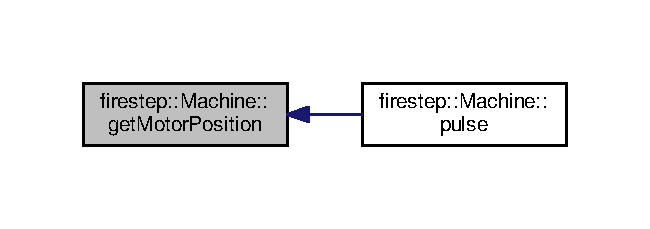
\includegraphics[width=312pt]{classfirestep_1_1_machine_abb9ab1d2cc47dca81eed644f0cc73a05_icgraph}
\end{center}
\end{figure}


\hypertarget{classfirestep_1_1_machine_a01596c1eb82ee853417f77404317c4ed}{\index{firestep\+::\+Machine@{firestep\+::\+Machine}!pulse@{pulse}}
\index{pulse@{pulse}!firestep\+::\+Machine@{firestep\+::\+Machine}}
\subsubsection[{pulse}]{\setlength{\rightskip}{0pt plus 5cm}Status Machine\+::pulse (
\begin{DoxyParamCaption}
\item[{{\bf Quad}$<$ Step\+Coord $>$ \&}]{pulses}
\end{DoxyParamCaption}
)}}\label{classfirestep_1_1_machine_a01596c1eb82ee853417f77404317c4ed}
Send stepper pulses without updating position. This is important for homing, test and calibration Return S\+T\+A\+T\+U\+S\+\_\+\+O\+K on success 

Here is the call graph for this function\+:\nopagebreak
\begin{figure}[H]
\begin{center}
\leavevmode
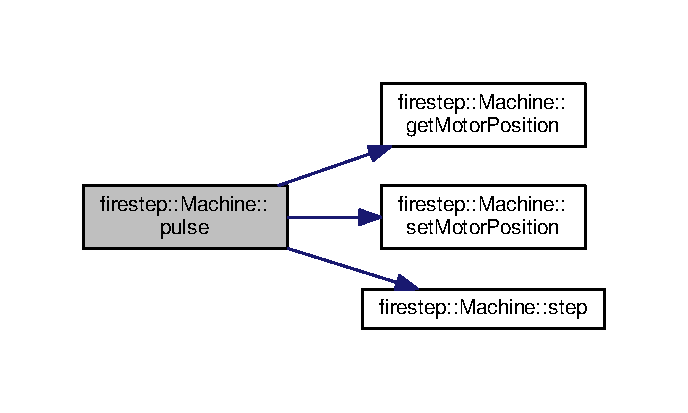
\includegraphics[width=330pt]{classfirestep_1_1_machine_a01596c1eb82ee853417f77404317c4ed_cgraph}
\end{center}
\end{figure}


\hypertarget{classfirestep_1_1_machine_a93b092c0652cb3abbe52169d41063462}{\index{firestep\+::\+Machine@{firestep\+::\+Machine}!set\+Home\+Angle@{set\+Home\+Angle}}
\index{set\+Home\+Angle@{set\+Home\+Angle}!firestep\+::\+Machine@{firestep\+::\+Machine}}
\subsubsection[{set\+Home\+Angle}]{\setlength{\rightskip}{0pt plus 5cm}void Machine\+::set\+Home\+Angle (
\begin{DoxyParamCaption}
\item[{P\+H5\+T\+Y\+P\+E}]{degrees}
\end{DoxyParamCaption}
)}}\label{classfirestep_1_1_machine_a93b092c0652cb3abbe52169d41063462}
Set the home angle and pulses 

Here is the caller graph for this function\+:
\nopagebreak
\begin{figure}[H]
\begin{center}
\leavevmode
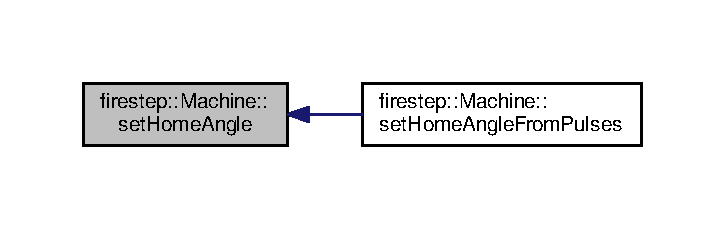
\includegraphics[width=348pt]{classfirestep_1_1_machine_a93b092c0652cb3abbe52169d41063462_icgraph}
\end{center}
\end{figure}


\hypertarget{classfirestep_1_1_machine_a85fbaf148788ffbdfe297d50a916238e}{\index{firestep\+::\+Machine@{firestep\+::\+Machine}!set\+Home\+Angle\+From\+Pulses@{set\+Home\+Angle\+From\+Pulses}}
\index{set\+Home\+Angle\+From\+Pulses@{set\+Home\+Angle\+From\+Pulses}!firestep\+::\+Machine@{firestep\+::\+Machine}}
\subsubsection[{set\+Home\+Angle\+From\+Pulses}]{\setlength{\rightskip}{0pt plus 5cm}void Machine\+::set\+Home\+Angle\+From\+Pulses (
\begin{DoxyParamCaption}
\item[{Step\+Coord}]{pulse\+Count}
\end{DoxyParamCaption}
)}}\label{classfirestep_1_1_machine_a85fbaf148788ffbdfe297d50a916238e}
Set the home pulses and angle. 

Here is the call graph for this function\+:
\nopagebreak
\begin{figure}[H]
\begin{center}
\leavevmode
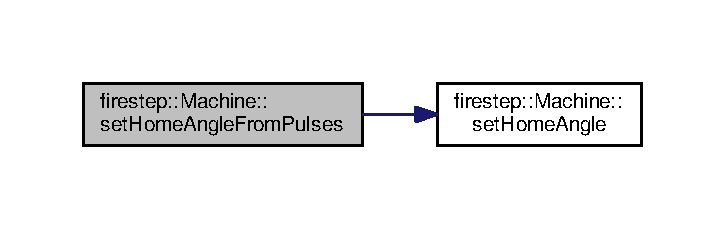
\includegraphics[width=348pt]{classfirestep_1_1_machine_a85fbaf148788ffbdfe297d50a916238e_cgraph}
\end{center}
\end{figure}


\hypertarget{classfirestep_1_1_machine_a6a92108622bf3dd555c32ffbea7b0f7a}{\index{firestep\+::\+Machine@{firestep\+::\+Machine}!set\+Motor\+Position@{set\+Motor\+Position}}
\index{set\+Motor\+Position@{set\+Motor\+Position}!firestep\+::\+Machine@{firestep\+::\+Machine}}
\subsubsection[{set\+Motor\+Position}]{\setlength{\rightskip}{0pt plus 5cm}void Machine\+::set\+Motor\+Position (
\begin{DoxyParamCaption}
\item[{const {\bf Quad}$<$ Step\+Coord $>$ \&}]{position}
\end{DoxyParamCaption}
)}}\label{classfirestep_1_1_machine_a6a92108622bf3dd555c32ffbea7b0f7a}
Set position of currently driven axes bound to motors 

Here is the caller graph for this function\+:\nopagebreak
\begin{figure}[H]
\begin{center}
\leavevmode
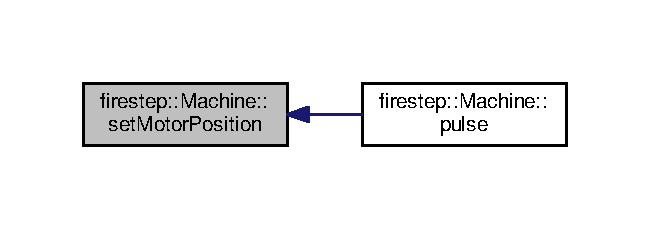
\includegraphics[width=312pt]{classfirestep_1_1_machine_a6a92108622bf3dd555c32ffbea7b0f7a_icgraph}
\end{center}
\end{figure}


\hypertarget{classfirestep_1_1_machine_a581b2333ca877f4ea4c020eaaaf485f3}{\index{firestep\+::\+Machine@{firestep\+::\+Machine}!step@{step}}
\index{step@{step}!firestep\+::\+Machine@{firestep\+::\+Machine}}
\subsubsection[{step}]{\setlength{\rightskip}{0pt plus 5cm}Status Machine\+::step (
\begin{DoxyParamCaption}
\item[{const {\bf Quad}$<$ Step\+D\+V $>$ \&}]{pulse}
\end{DoxyParamCaption}
)\hspace{0.3cm}{\ttfamily [virtual]}}}\label{classfirestep_1_1_machine_a581b2333ca877f4ea4c020eaaaf485f3}
The \hyperlink{classfirestep_1_1_machine_a581b2333ca877f4ea4c020eaaaf485f3}{step()} method is the \char`\"{}stepper inner loop\char`\"{} that creates the stepper pulse train to Q\+U\+A\+D\+\_\+\+E\+L\+E\+M\+E\+N\+T\+S steppers. The pulse parameter must have a value of -\/1, 0, or 1 for each stepper.

Steppers can't be driven too quickly--they stall. Each axis has a us\+Delay field that specifies a minimum delay between pulses. 

Implements \hyperlink{classfirestep_1_1_quad_stepper}{firestep\+::\+Quad\+Stepper}.



Here is the caller graph for this function\+:\nopagebreak
\begin{figure}[H]
\begin{center}
\leavevmode
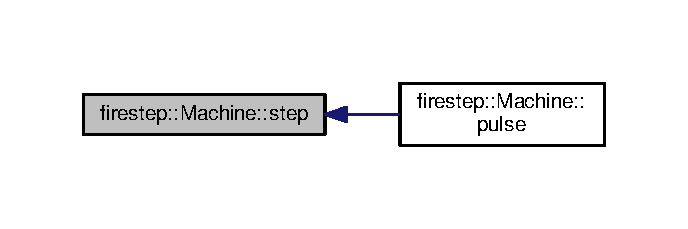
\includegraphics[width=330pt]{classfirestep_1_1_machine_a581b2333ca877f4ea4c020eaaaf485f3_icgraph}
\end{center}
\end{figure}


\hypertarget{classfirestep_1_1_machine_ad3cfb55e4071b4d20855175beb21ed6a}{\index{firestep\+::\+Machine@{firestep\+::\+Machine}!step\+Direction@{step\+Direction}}
\index{step\+Direction@{step\+Direction}!firestep\+::\+Machine@{firestep\+::\+Machine}}
\subsubsection[{step\+Direction}]{\setlength{\rightskip}{0pt plus 5cm}Status Machine\+::step\+Direction (
\begin{DoxyParamCaption}
\item[{const {\bf Quad}$<$ Step\+D\+V $>$ \&}]{pulse}
\end{DoxyParamCaption}
)\hspace{0.3cm}{\ttfamily [virtual]}}}\label{classfirestep_1_1_machine_ad3cfb55e4071b4d20855175beb21ed6a}
Set direction based on the sign of each pulse value and check bounds 

Implements \hyperlink{classfirestep_1_1_quad_stepper}{firestep\+::\+Quad\+Stepper}.



The documentation for this class was generated from the following files\+:\begin{DoxyCompactItemize}
\item 
Machine.\+h\item 
Machine.\+cpp\end{DoxyCompactItemize}

\hypertarget{classfirestep_1_1_machine_thread}{\section{firestep\+:\+:Machine\+Thread Class Reference}
\label{classfirestep_1_1_machine_thread}\index{firestep\+::\+Machine\+Thread@{firestep\+::\+Machine\+Thread}}
}


Inheritance diagram for firestep\+:\+:Machine\+Thread\+:\nopagebreak
\begin{figure}[H]
\begin{center}
\leavevmode
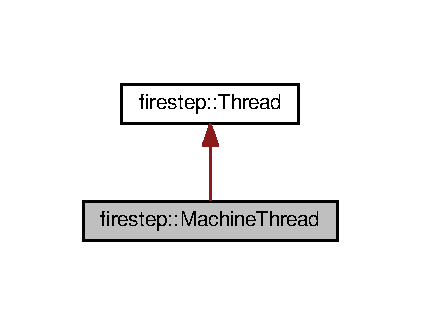
\includegraphics[width=202pt]{classfirestep_1_1_machine_thread__inherit__graph}
\end{center}
\end{figure}


Collaboration diagram for firestep\+:\+:Machine\+Thread\+:
\nopagebreak
\begin{figure}[H]
\begin{center}
\leavevmode
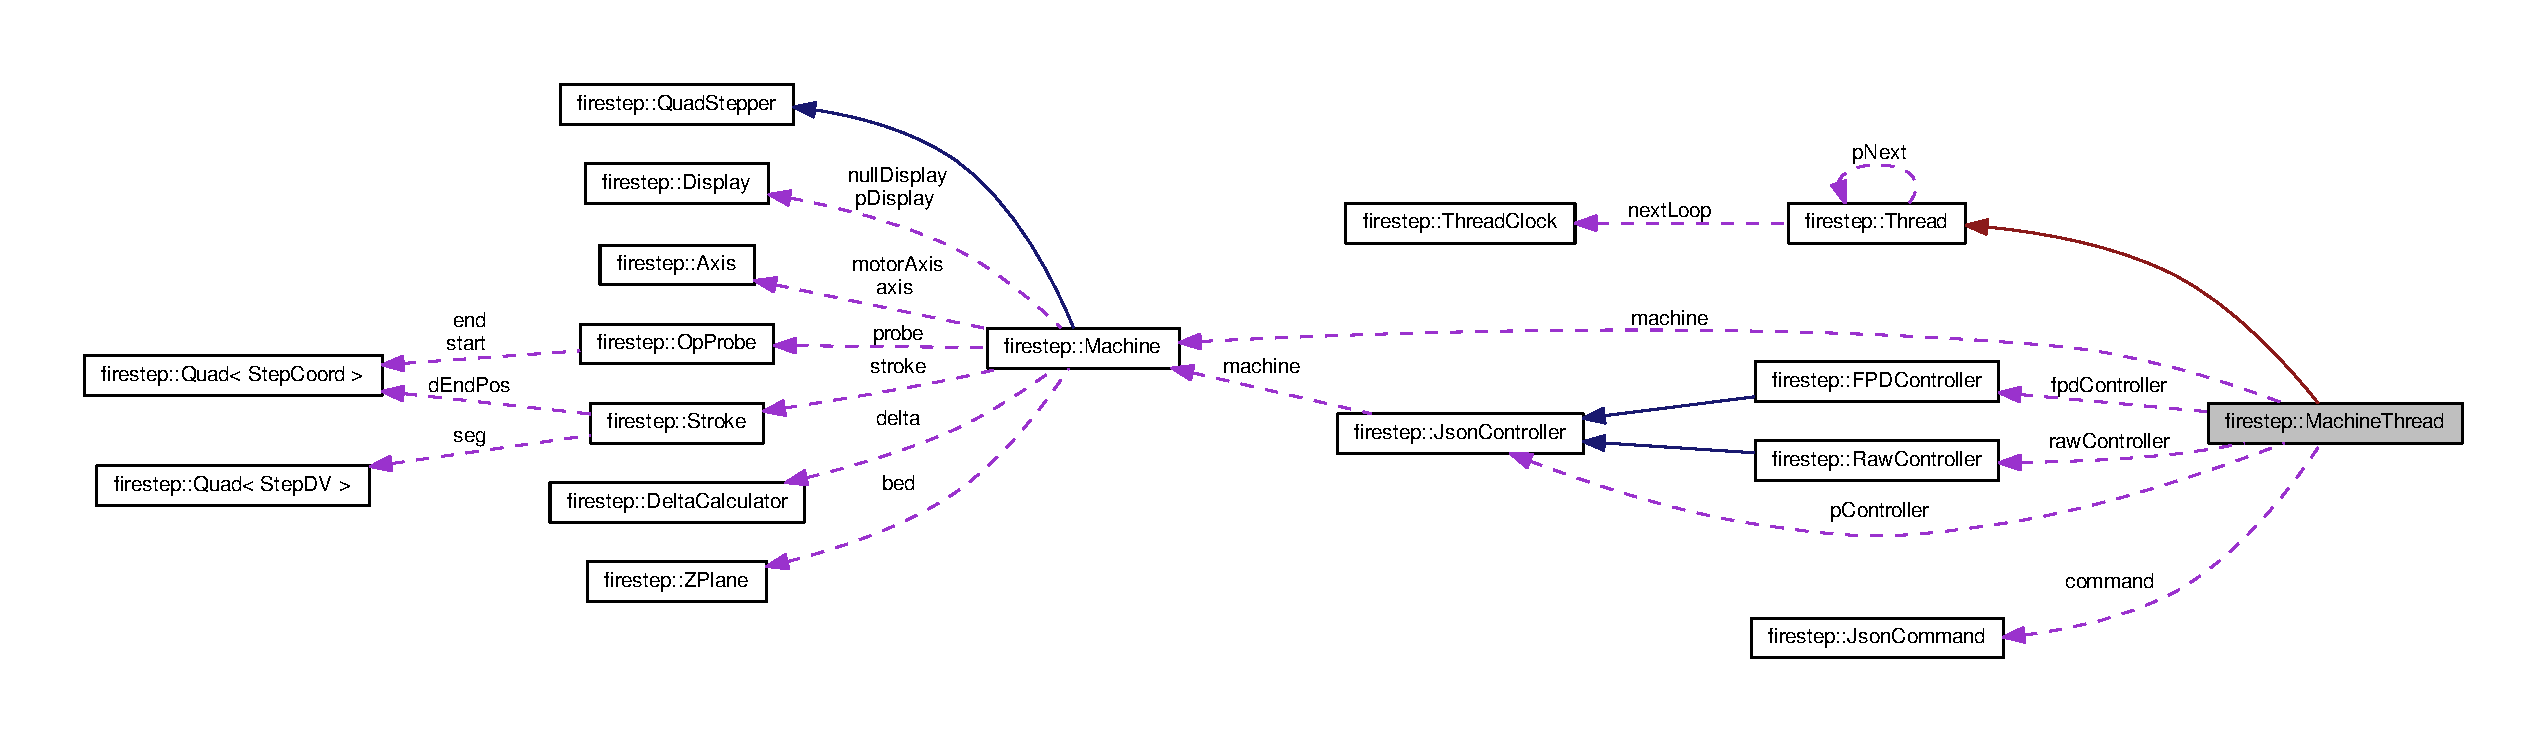
\includegraphics[width=350pt]{classfirestep_1_1_machine_thread__coll__graph}
\end{center}
\end{figure}
\subsection*{Public Member Functions}
\begin{DoxyCompactItemize}
\item 
\hypertarget{classfirestep_1_1_machine_thread_a4fe579c1ee6423fb2ce41280b5301067}{void {\bfseries set\+Controller} (\hyperlink{classfirestep_1_1_json_controller}{Json\+Controller} \&controller)}\label{classfirestep_1_1_machine_thread_a4fe579c1ee6423fb2ce41280b5301067}

\item 
\hypertarget{classfirestep_1_1_machine_thread_a8bb7b8030b3277891792bee0584229f3}{void {\bfseries setup} (Pin\+Config pc)}\label{classfirestep_1_1_machine_thread_a8bb7b8030b3277891792bee0584229f3}

\item 
\hypertarget{classfirestep_1_1_machine_thread_ab7dab8e7bc91e51ba49f9e1f0cb93661}{void {\bfseries loop} ()}\label{classfirestep_1_1_machine_thread_ab7dab8e7bc91e51ba49f9e1f0cb93661}

\item 
\hypertarget{classfirestep_1_1_machine_thread_a5d667c949b4c23e053e82688154c7236}{Status {\bfseries sync\+Config} ()}\label{classfirestep_1_1_machine_thread_a5d667c949b4c23e053e82688154c7236}

\item 
\hypertarget{classfirestep_1_1_machine_thread_a97b101bb4bc51dc8c46d018a7af3aa24}{Status {\bfseries process} (\hyperlink{classfirestep_1_1_json_command}{Json\+Command} \&jcmd)}\label{classfirestep_1_1_machine_thread_a97b101bb4bc51dc8c46d018a7af3aa24}

\item 
\hypertarget{classfirestep_1_1_machine_thread_a31916705d92cd50bce1ea6609de2b5d5}{const char $\ast$ {\bfseries update\+Controller} ()}\label{classfirestep_1_1_machine_thread_a31916705d92cd50bce1ea6609de2b5d5}

\end{DoxyCompactItemize}
\subsection*{Public Attributes}
\begin{DoxyCompactItemize}
\item 
\hypertarget{classfirestep_1_1_machine_thread_a5253f82dc2425a663360c24a7f406667}{Status {\bfseries status}}\label{classfirestep_1_1_machine_thread_a5253f82dc2425a663360c24a7f406667}

\item 
\hypertarget{classfirestep_1_1_machine_thread_ac4c826e67411f9241a31784923d0a0d9}{\hyperlink{classfirestep_1_1_machine}{Machine} {\bfseries machine}}\label{classfirestep_1_1_machine_thread_ac4c826e67411f9241a31784923d0a0d9}

\item 
\hypertarget{classfirestep_1_1_machine_thread_a7c2d7afb44d03213dc502275ba9e8675}{\hyperlink{classfirestep_1_1_json_command}{Json\+Command} {\bfseries command}}\label{classfirestep_1_1_machine_thread_a7c2d7afb44d03213dc502275ba9e8675}

\item 
\hypertarget{classfirestep_1_1_machine_thread_a88db4fa4d2b7d440ad36fe67f7db686c}{\hyperlink{classfirestep_1_1_raw_controller}{Raw\+Controller} {\bfseries raw\+Controller}}\label{classfirestep_1_1_machine_thread_a88db4fa4d2b7d440ad36fe67f7db686c}

\item 
\hypertarget{classfirestep_1_1_machine_thread_adf38017962b0c7fa074ae114601bfd25}{\hyperlink{classfirestep_1_1_f_p_d_controller}{F\+P\+D\+Controller} {\bfseries fpd\+Controller}}\label{classfirestep_1_1_machine_thread_adf38017962b0c7fa074ae114601bfd25}

\item 
\hypertarget{classfirestep_1_1_machine_thread_a52d6e74762eb5485a14b5706336cd7de}{\hyperlink{classfirestep_1_1_json_controller}{Json\+Controller} $\ast$ {\bfseries p\+Controller}}\label{classfirestep_1_1_machine_thread_a52d6e74762eb5485a14b5706336cd7de}

\item 
\hypertarget{classfirestep_1_1_machine_thread_a01318c47c8e1bb55d4f5098a02136cd8}{bool {\bfseries print\+Banner\+On\+Idle}}\label{classfirestep_1_1_machine_thread_a01318c47c8e1bb55d4f5098a02136cd8}

\end{DoxyCompactItemize}
\subsection*{Protected Member Functions}
\begin{DoxyCompactItemize}
\item 
\hypertarget{classfirestep_1_1_machine_thread_a7bcbd1dcbab0e5a19219311b228e41e7}{void {\bfseries display\+Status} ()}\label{classfirestep_1_1_machine_thread_a7bcbd1dcbab0e5a19219311b228e41e7}

\item 
\hypertarget{classfirestep_1_1_machine_thread_adf8a53b9a4707e08b71485a3f6346653}{char $\ast$ {\bfseries build\+Startup\+Json} ()}\label{classfirestep_1_1_machine_thread_adf8a53b9a4707e08b71485a3f6346653}

\item 
\hypertarget{classfirestep_1_1_machine_thread_a5748af706dc5b71a7acaa310436556c9}{Status {\bfseries execute\+E\+E\+P\+R\+O\+M} ()}\label{classfirestep_1_1_machine_thread_a5748af706dc5b71a7acaa310436556c9}

\item 
\hypertarget{classfirestep_1_1_machine_thread_ac72394eda14bc0be7569243db6a057a0}{size\+\_\+t {\bfseries read\+E\+E\+P\+R\+O\+M} (uint8\+\_\+t $\ast$eeprom\+\_\+addr, char $\ast$dst, size\+\_\+t max\+Len)}\label{classfirestep_1_1_machine_thread_ac72394eda14bc0be7569243db6a057a0}

\end{DoxyCompactItemize}
\subsection*{Friends}
\begin{DoxyCompactItemize}
\item 
\hypertarget{classfirestep_1_1_machine_thread_a018c6a85067bcfc99f7d5a3753ce766d}{void {\bfseries test\+\_\+\+Home} ()}\label{classfirestep_1_1_machine_thread_a018c6a85067bcfc99f7d5a3753ce766d}

\end{DoxyCompactItemize}


The documentation for this class was generated from the following files\+:\begin{DoxyCompactItemize}
\item 
Machine\+Thread.\+h\item 
Machine\+Thread.\+cpp\end{DoxyCompactItemize}

\hypertarget{classfirestep_1_1_monitor_thread}{\section{firestep\+:\+:Monitor\+Thread Class Reference}
\label{classfirestep_1_1_monitor_thread}\index{firestep\+::\+Monitor\+Thread@{firestep\+::\+Monitor\+Thread}}
}


Inheritance diagram for firestep\+:\+:Monitor\+Thread\+:\nopagebreak
\begin{figure}[H]
\begin{center}
\leavevmode
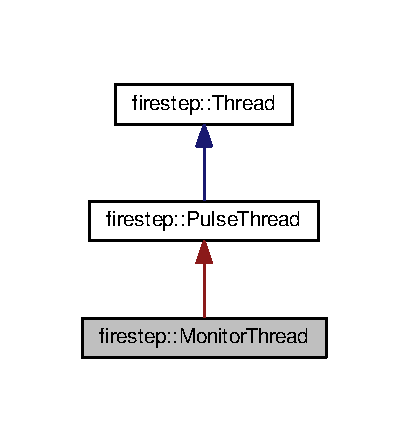
\includegraphics[width=196pt]{classfirestep_1_1_monitor_thread__inherit__graph}
\end{center}
\end{figure}


Collaboration diagram for firestep\+:\+:Monitor\+Thread\+:\nopagebreak
\begin{figure}[H]
\begin{center}
\leavevmode
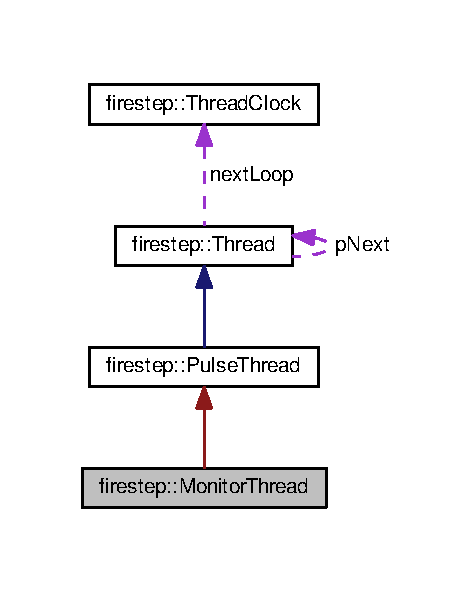
\includegraphics[width=228pt]{classfirestep_1_1_monitor_thread__coll__graph}
\end{center}
\end{figure}
\subsection*{Public Member Functions}
\begin{DoxyCompactItemize}
\item 
\hypertarget{classfirestep_1_1_monitor_thread_aeec0a226aa0a63a649b9c0ee83a9f185}{void {\bfseries Error} (const char $\ast$msg, int value)}\label{classfirestep_1_1_monitor_thread_aeec0a226aa0a63a649b9c0ee83a9f185}

\end{DoxyCompactItemize}
\subsection*{Public Attributes}
\begin{DoxyCompactItemize}
\item 
\hypertarget{classfirestep_1_1_monitor_thread_a7c6ab8de3d6a340f3937a8b7f14103ee}{bool {\bfseries verbose}}\label{classfirestep_1_1_monitor_thread_a7c6ab8de3d6a340f3937a8b7f14103ee}

\end{DoxyCompactItemize}
\subsection*{Friends}
\begin{DoxyCompactItemize}
\item 
\hypertarget{classfirestep_1_1_monitor_thread_ae32f2b9b26ebd4cd05a23ee82797622d}{class {\bfseries Thread\+Runner}}\label{classfirestep_1_1_monitor_thread_ae32f2b9b26ebd4cd05a23ee82797622d}

\item 
\hypertarget{classfirestep_1_1_monitor_thread_aef06a3028e2da14682b40e8349d0c8c0}{class {\bfseries Machine\+Thread}}\label{classfirestep_1_1_monitor_thread_aef06a3028e2da14682b40e8349d0c8c0}

\end{DoxyCompactItemize}


The documentation for this class was generated from the following files\+:\begin{DoxyCompactItemize}
\item 
Thread.\+h\item 
Thread.\+cpp\end{DoxyCompactItemize}

\hypertarget{class_m_t_o___r_a_w_move_to}{\section{M\+T\+O\+\_\+\+R\+A\+W\+Move\+To Class Reference}
\label{class_m_t_o___r_a_w_move_to}\index{M\+T\+O\+\_\+\+R\+A\+W\+Move\+To@{M\+T\+O\+\_\+\+R\+A\+W\+Move\+To}}
}
\subsection*{Public Member Functions}
\begin{DoxyCompactItemize}
\item 
\hypertarget{class_m_t_o___r_a_w_move_to_a8ae04f16f348d6a18610bc8689e8a412}{{\bfseries M\+T\+O\+\_\+\+R\+A\+W\+Move\+To} (\hyperlink{classfirestep_1_1_machine}{Machine} \&machine)}\label{class_m_t_o___r_a_w_move_to_a8ae04f16f348d6a18610bc8689e8a412}

\item 
\hypertarget{class_m_t_o___r_a_w_move_to_a06a7927d5cd8575ab3d9ec290316ccf9}{Status {\bfseries process} (\hyperlink{classfirestep_1_1_json_command}{Json\+Command} \&jcmd, Json\+Object \&jobj, const char $\ast$key)}\label{class_m_t_o___r_a_w_move_to_a06a7927d5cd8575ab3d9ec290316ccf9}

\end{DoxyCompactItemize}


The documentation for this class was generated from the following file\+:\begin{DoxyCompactItemize}
\item 
Raw\+Controller.\+cpp\end{DoxyCompactItemize}

\hypertarget{classfirestep_1_1_neo_pixel}{\section{firestep\+:\+:Neo\+Pixel Class Reference}
\label{classfirestep_1_1_neo_pixel}\index{firestep\+::\+Neo\+Pixel@{firestep\+::\+Neo\+Pixel}}
}


Inheritance diagram for firestep\+:\+:Neo\+Pixel\+:\nopagebreak
\begin{figure}[H]
\begin{center}
\leavevmode
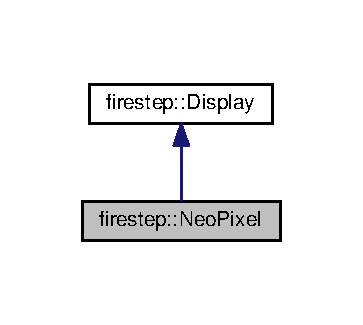
\includegraphics[width=174pt]{classfirestep_1_1_neo_pixel__inherit__graph}
\end{center}
\end{figure}


Collaboration diagram for firestep\+:\+:Neo\+Pixel\+:\nopagebreak
\begin{figure}[H]
\begin{center}
\leavevmode
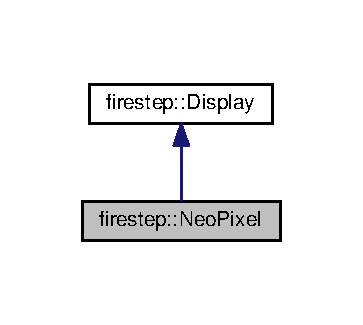
\includegraphics[width=174pt]{classfirestep_1_1_neo_pixel__coll__graph}
\end{center}
\end{figure}
\subsection*{Public Member Functions}
\begin{DoxyCompactItemize}
\item 
\hypertarget{classfirestep_1_1_neo_pixel_af4205fe9853612babdda3db19b7d0b95}{{\bfseries Neo\+Pixel} (uint16\+\_\+t led\+Count)}\label{classfirestep_1_1_neo_pixel_af4205fe9853612babdda3db19b7d0b95}

\item 
\hypertarget{classfirestep_1_1_neo_pixel_aef35dca3b6a1cf79a7c8cad2010600d5}{void {\bfseries setup} (int pin)}\label{classfirestep_1_1_neo_pixel_aef35dca3b6a1cf79a7c8cad2010600d5}

\item 
\hypertarget{classfirestep_1_1_neo_pixel_a56ef3d39dfee07f276165f38569087b0}{void {\bfseries show} ()}\label{classfirestep_1_1_neo_pixel_a56ef3d39dfee07f276165f38569087b0}

\end{DoxyCompactItemize}
\subsection*{Protected Attributes}
\begin{DoxyCompactItemize}
\item 
\hypertarget{classfirestep_1_1_neo_pixel_a42ac6f7e29d6579ee6c9b3b2c36cc38e}{Adafruit\+\_\+\+Neo\+Pixel {\bfseries strip}}\label{classfirestep_1_1_neo_pixel_a42ac6f7e29d6579ee6c9b3b2c36cc38e}

\item 
\hypertarget{classfirestep_1_1_neo_pixel_a20e98401689568572b8f7a4fafdcdd12}{uint8\+\_\+t {\bfseries cur\+Level}}\label{classfirestep_1_1_neo_pixel_a20e98401689568572b8f7a4fafdcdd12}

\item 
\hypertarget{classfirestep_1_1_neo_pixel_ad1f830a67f5de8e6ec7bc800f8494805}{uint8\+\_\+t {\bfseries cur\+Status}}\label{classfirestep_1_1_neo_pixel_ad1f830a67f5de8e6ec7bc800f8494805}

\item 
\hypertarget{classfirestep_1_1_neo_pixel_acafe96dea7f2f5e9d7d8ee14109923be}{uint8\+\_\+t {\bfseries fg\+Index}}\label{classfirestep_1_1_neo_pixel_acafe96dea7f2f5e9d7d8ee14109923be}

\item 
\hypertarget{classfirestep_1_1_neo_pixel_a668b995080132555a333b4628e9a615f}{uint32\+\_\+t {\bfseries fg\+Millis}}\label{classfirestep_1_1_neo_pixel_a668b995080132555a333b4628e9a615f}

\item 
\hypertarget{classfirestep_1_1_neo_pixel_a77bf9d6ccf80f93bda14bf42cd59c943}{uint32\+\_\+t {\bfseries fg}}\label{classfirestep_1_1_neo_pixel_a77bf9d6ccf80f93bda14bf42cd59c943}

\item 
\hypertarget{classfirestep_1_1_neo_pixel_a234897f0de7c449f81cef5f75f76eec5}{uint32\+\_\+t {\bfseries bg}}\label{classfirestep_1_1_neo_pixel_a234897f0de7c449f81cef5f75f76eec5}

\end{DoxyCompactItemize}


The documentation for this class was generated from the following files\+:\begin{DoxyCompactItemize}
\item 
Neo\+Pixel.\+h\item 
Neo\+Pixel.\+cpp\end{DoxyCompactItemize}

\hypertarget{classfirestep_1_1_op_probe}{\section{firestep\+:\+:Op\+Probe Class Reference}
\label{classfirestep_1_1_op_probe}\index{firestep\+::\+Op\+Probe@{firestep\+::\+Op\+Probe}}
}


Collaboration diagram for firestep\+:\+:Op\+Probe\+:\nopagebreak
\begin{figure}[H]
\begin{center}
\leavevmode
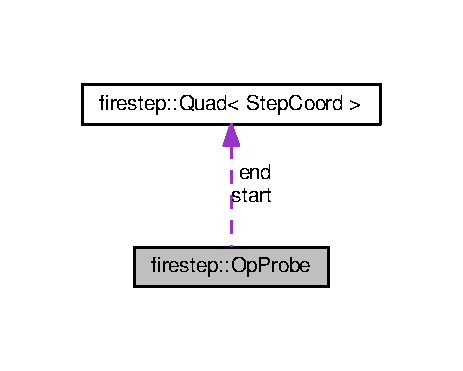
\includegraphics[width=222pt]{classfirestep_1_1_op_probe__coll__graph}
\end{center}
\end{figure}
\subsection*{Public Member Functions}
\begin{DoxyCompactItemize}
\item 
\hypertarget{classfirestep_1_1_op_probe_a458ffa766ae074c300380d9b2d0f0225}{void {\bfseries setup} (\hyperlink{classfirestep_1_1_quad}{Quad}$<$ Step\+Coord $>$ pos\+Start)}\label{classfirestep_1_1_op_probe_a458ffa766ae074c300380d9b2d0f0225}

\item 
\hypertarget{classfirestep_1_1_op_probe_a1791ea37a015521b021931dec1831077}{void {\bfseries setup} (\hyperlink{classfirestep_1_1_quad}{Quad}$<$ Step\+Coord $>$ pos\+Start, \hyperlink{classfirestep_1_1_quad}{Quad}$<$ Step\+Coord $>$ pos\+End)}\label{classfirestep_1_1_op_probe_a1791ea37a015521b021931dec1831077}

\item 
\hypertarget{classfirestep_1_1_op_probe_a3785370d148fcce00bade62b66a46357}{Step\+Coord {\bfseries interpolate} (Motor\+Index i\+Motor)}\label{classfirestep_1_1_op_probe_a3785370d148fcce00bade62b66a46357}

\item 
\hypertarget{classfirestep_1_1_op_probe_a4765e688e5391866353afd36dddf2a77}{void {\bfseries archive\+Data} (P\+H5\+T\+Y\+P\+E data)}\label{classfirestep_1_1_op_probe_a4765e688e5391866353afd36dddf2a77}

\end{DoxyCompactItemize}
\subsection*{Public Attributes}
\begin{DoxyCompactItemize}
\item 
\hypertarget{classfirestep_1_1_op_probe_a54509accd4d8988a7e9922b321dba8cc}{\hyperlink{classfirestep_1_1_quad}{Quad}$<$ Step\+Coord $>$ {\bfseries start}}\label{classfirestep_1_1_op_probe_a54509accd4d8988a7e9922b321dba8cc}

\item 
\hypertarget{classfirestep_1_1_op_probe_ab0bc3730b2de1f56bb04f4b2dce6e5ae}{\hyperlink{classfirestep_1_1_quad}{Quad}$<$ Step\+Coord $>$ {\bfseries end}}\label{classfirestep_1_1_op_probe_ab0bc3730b2de1f56bb04f4b2dce6e5ae}

\item 
\hypertarget{classfirestep_1_1_op_probe_aec7d6e41e2a0ad41cca58bc5bc6fbd47}{Step\+Coord {\bfseries max\+Delta}}\label{classfirestep_1_1_op_probe_aec7d6e41e2a0ad41cca58bc5bc6fbd47}

\item 
\hypertarget{classfirestep_1_1_op_probe_a2058a896655a2d893a4171a28115b00e}{Step\+Coord {\bfseries cur\+Delta}}\label{classfirestep_1_1_op_probe_a2058a896655a2d893a4171a28115b00e}

\item 
\hypertarget{classfirestep_1_1_op_probe_a3eef6faa8f450dd1418160c64e6b1e85}{Pin\+Type {\bfseries pin\+Probe}}\label{classfirestep_1_1_op_probe_a3eef6faa8f450dd1418160c64e6b1e85}

\item 
\hypertarget{classfirestep_1_1_op_probe_a0da566d41c33ea1902678677374ac2b8}{Probe\+Data\+Source {\bfseries data\+Source}}\label{classfirestep_1_1_op_probe_a0da566d41c33ea1902678677374ac2b8}

\item 
\hypertarget{classfirestep_1_1_op_probe_ae19616ba52b69ef0b51e1a47f030a207}{bool {\bfseries probing}}\label{classfirestep_1_1_op_probe_ae19616ba52b69ef0b51e1a47f030a207}

\item 
\hypertarget{classfirestep_1_1_op_probe_a6526a2c2745fc1844432d740a8a7a2e4}{bool {\bfseries invert\+Probe}}\label{classfirestep_1_1_op_probe_a6526a2c2745fc1844432d740a8a7a2e4}

\item 
\hypertarget{classfirestep_1_1_op_probe_a09468bc0628d58d264bb1d5d02da8726}{P\+H5\+T\+Y\+P\+E {\bfseries probe\+Data} \mbox{[}P\+R\+O\+B\+E\+\_\+\+D\+A\+T\+A\mbox{]}}\label{classfirestep_1_1_op_probe_a09468bc0628d58d264bb1d5d02da8726}

\end{DoxyCompactItemize}


The documentation for this class was generated from the following file\+:\begin{DoxyCompactItemize}
\item 
Machine.\+h\end{DoxyCompactItemize}

\hypertarget{class_p_h_self_test}{\section{P\+H\+Self\+Test Class Reference}
\label{class_p_h_self_test}\index{P\+H\+Self\+Test@{P\+H\+Self\+Test}}
}
\subsection*{Public Member Functions}
\begin{DoxyCompactItemize}
\item 
\hypertarget{class_p_h_self_test_a2b35b015c8453d513259249b2e14e779}{{\bfseries P\+H\+Self\+Test} (\hyperlink{classfirestep_1_1_machine}{Machine} \&machine)}\label{class_p_h_self_test_a2b35b015c8453d513259249b2e14e779}

\item 
\hypertarget{class_p_h_self_test_a6ad22cb23f5d4d9e782079b6bc81f873}{Status {\bfseries process} (\hyperlink{classfirestep_1_1_json_command}{Json\+Command} \&jcmd, Json\+Object \&jobj, const char $\ast$key)}\label{class_p_h_self_test_a6ad22cb23f5d4d9e782079b6bc81f873}

\end{DoxyCompactItemize}


The documentation for this class was generated from the following file\+:\begin{DoxyCompactItemize}
\item 
Json\+Controller.\+cpp\end{DoxyCompactItemize}

\hypertarget{structfirestep_1_1_pulse_thread}{\section{firestep\+:\+:Pulse\+Thread Struct Reference}
\label{structfirestep_1_1_pulse_thread}\index{firestep\+::\+Pulse\+Thread@{firestep\+::\+Pulse\+Thread}}
}


Inheritance diagram for firestep\+:\+:Pulse\+Thread\+:\nopagebreak
\begin{figure}[H]
\begin{center}
\leavevmode
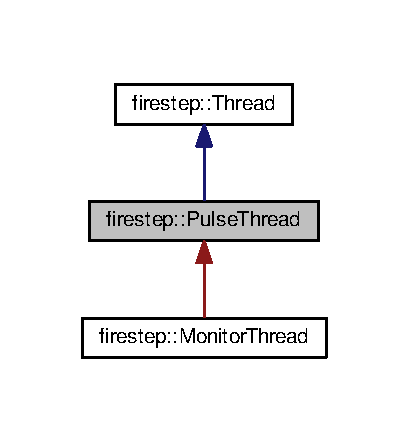
\includegraphics[width=196pt]{structfirestep_1_1_pulse_thread__inherit__graph}
\end{center}
\end{figure}


Collaboration diagram for firestep\+:\+:Pulse\+Thread\+:\nopagebreak
\begin{figure}[H]
\begin{center}
\leavevmode
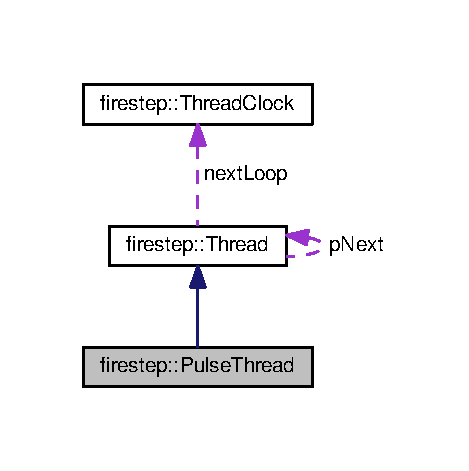
\includegraphics[width=225pt]{structfirestep_1_1_pulse_thread__coll__graph}
\end{center}
\end{figure}
\subsection*{Public Member Functions}
\begin{DoxyCompactItemize}
\item 
\hypertarget{structfirestep_1_1_pulse_thread_a818deb02f6bf4d8e646e9ca9ed1d1305}{virtual void {\bfseries setup} (Ticks period, Ticks pulse\+Width)}\label{structfirestep_1_1_pulse_thread_a818deb02f6bf4d8e646e9ca9ed1d1305}

\item 
\hypertarget{structfirestep_1_1_pulse_thread_acfca17547b41025ac398c4217558604c}{virtual void {\bfseries loop} ()}\label{structfirestep_1_1_pulse_thread_acfca17547b41025ac398c4217558604c}

\end{DoxyCompactItemize}
\subsection*{Public Attributes}
\begin{DoxyCompactItemize}
\item 
\hypertarget{structfirestep_1_1_pulse_thread_a28811f78e9b136829a192389dc0f941f}{bool {\bfseries is\+High}}\label{structfirestep_1_1_pulse_thread_a28811f78e9b136829a192389dc0f941f}

\end{DoxyCompactItemize}
\subsection*{Protected Attributes}
\begin{DoxyCompactItemize}
\item 
\hypertarget{structfirestep_1_1_pulse_thread_ade79afaef23c6cdc7bb12e77e148bd5b}{Ticks {\bfseries m\+\_\+\+Low\+Period}}\label{structfirestep_1_1_pulse_thread_ade79afaef23c6cdc7bb12e77e148bd5b}

\item 
\hypertarget{structfirestep_1_1_pulse_thread_a3b0898a4a995c26f6324f0996f01df83}{Ticks {\bfseries m\+\_\+\+High\+Period}}\label{structfirestep_1_1_pulse_thread_a3b0898a4a995c26f6324f0996f01df83}

\end{DoxyCompactItemize}


The documentation for this struct was generated from the following files\+:\begin{DoxyCompactItemize}
\item 
Thread.\+h\item 
Thread.\+cpp\end{DoxyCompactItemize}

\hypertarget{classfirestep_1_1_quad}{\section{firestep\+:\+:Quad$<$ T $>$ Class Template Reference}
\label{classfirestep_1_1_quad}\index{firestep\+::\+Quad$<$ T $>$@{firestep\+::\+Quad$<$ T $>$}}
}


Collaboration diagram for firestep\+:\+:Quad$<$ T $>$\+:\nopagebreak
\begin{figure}[H]
\begin{center}
\leavevmode
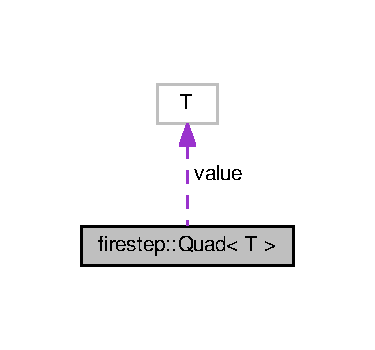
\includegraphics[width=180pt]{classfirestep_1_1_quad__coll__graph}
\end{center}
\end{figure}
\subsection*{Public Member Functions}
\begin{DoxyCompactItemize}
\item 
\hypertarget{classfirestep_1_1_quad_ad4a5fe8b71084308636c549ed9139b62}{{\bfseries Quad} (T v1=0, T v2=0, T v3=0, T v4=0)}\label{classfirestep_1_1_quad_ad4a5fe8b71084308636c549ed9139b62}

\item 
\hypertarget{classfirestep_1_1_quad_a0df9f8f9f5f01600bca23a5ece1d7f93}{bool {\bfseries is\+Zero} ()}\label{classfirestep_1_1_quad_a0df9f8f9f5f01600bca23a5ece1d7f93}

\item 
\hypertarget{classfirestep_1_1_quad_a18c27f35b1e58bb9d7fa41f2d33e1778}{\hyperlink{classfirestep_1_1_quad}{Quad}$<$ T $>$ {\bfseries sgn} ()}\label{classfirestep_1_1_quad_a18c27f35b1e58bb9d7fa41f2d33e1778}

\item 
\hypertarget{classfirestep_1_1_quad_ae51176822861d549a29b5ceac77770ab}{\hyperlink{classfirestep_1_1_quad}{Quad}$<$ T $>$ {\bfseries absolute\+Value} ()}\label{classfirestep_1_1_quad_ae51176822861d549a29b5ceac77770ab}

\item 
\hypertarget{classfirestep_1_1_quad_a6e51be6ab5dfd2114f2726562934207e}{float {\bfseries norm2} ()}\label{classfirestep_1_1_quad_a6e51be6ab5dfd2114f2726562934207e}

\item 
\hypertarget{classfirestep_1_1_quad_a35a4acb760021be2709db0eb46973c8c}{void {\bfseries clear} ()}\label{classfirestep_1_1_quad_a35a4acb760021be2709db0eb46973c8c}

\item 
\hypertarget{classfirestep_1_1_quad_a04bf97b01c806383da66b2faaed1e61a}{\hyperlink{classfirestep_1_1_quad}{Quad}$<$ T $>$ {\bfseries operator+} (const \hyperlink{classfirestep_1_1_quad}{Quad}$<$ T $>$ \&that)}\label{classfirestep_1_1_quad_a04bf97b01c806383da66b2faaed1e61a}

\item 
\hypertarget{classfirestep_1_1_quad_a1db197c5eff89aa649ab149665ea8a66}{\hyperlink{classfirestep_1_1_quad}{Quad}$<$ T $>$ {\bfseries operator-\/} (const \hyperlink{classfirestep_1_1_quad}{Quad}$<$ T $>$ \&that)}\label{classfirestep_1_1_quad_a1db197c5eff89aa649ab149665ea8a66}

\item 
\hypertarget{classfirestep_1_1_quad_abfbc5902b39995e7ccc1d3a0de311165}{\hyperlink{classfirestep_1_1_quad}{Quad}$<$ T $>$ \& {\bfseries operator=} (T that)}\label{classfirestep_1_1_quad_abfbc5902b39995e7ccc1d3a0de311165}

\item 
\hypertarget{classfirestep_1_1_quad_aa49ba6313524d4e47f7e80651f656eed}{\hyperlink{classfirestep_1_1_quad}{Quad}$<$ T $>$ \& {\bfseries operator=} (const \hyperlink{classfirestep_1_1_quad}{Quad}$<$ T $>$ \&that)}\label{classfirestep_1_1_quad_aa49ba6313524d4e47f7e80651f656eed}

\item 
\hypertarget{classfirestep_1_1_quad_acf4f7e0630ed4ead88b2f3dc784ee80e}{\hyperlink{classfirestep_1_1_quad}{Quad}$<$ T $>$ {\bfseries operator$\ast$} (T that)}\label{classfirestep_1_1_quad_acf4f7e0630ed4ead88b2f3dc784ee80e}

\item 
\hypertarget{classfirestep_1_1_quad_a7b39552fc122dbe845e0a77dcf96aacb}{\hyperlink{classfirestep_1_1_quad}{Quad}$<$ T $>$ \& {\bfseries operator$\ast$=} (T that)}\label{classfirestep_1_1_quad_a7b39552fc122dbe845e0a77dcf96aacb}

\item 
\hypertarget{classfirestep_1_1_quad_ae619e27bba0f1981569a56025572c803}{\hyperlink{classfirestep_1_1_quad}{Quad}$<$ T $>$ \& {\bfseries operator/=} (T that)}\label{classfirestep_1_1_quad_ae619e27bba0f1981569a56025572c803}

\item 
\hypertarget{classfirestep_1_1_quad_abe6b69b5707b71899dfad30f0e77cf0b}{\hyperlink{classfirestep_1_1_quad}{Quad}$<$ T $>$ \& {\bfseries operator+=} (T that)}\label{classfirestep_1_1_quad_abe6b69b5707b71899dfad30f0e77cf0b}

\item 
\hypertarget{classfirestep_1_1_quad_a0057f45c1634052af5b9d6f98111ee69}{\hyperlink{classfirestep_1_1_quad}{Quad}$<$ T $>$ \& {\bfseries operator+=} (const \hyperlink{classfirestep_1_1_quad}{Quad}$<$ T $>$ \&that)}\label{classfirestep_1_1_quad_a0057f45c1634052af5b9d6f98111ee69}

\item 
\hypertarget{classfirestep_1_1_quad_a75aa9c24ad6035ef5ce4d82dfd47b87d}{\hyperlink{classfirestep_1_1_quad}{Quad}$<$ T $>$ \& {\bfseries operator-\/=} (const \hyperlink{classfirestep_1_1_quad}{Quad}$<$ T $>$ \&that)}\label{classfirestep_1_1_quad_a75aa9c24ad6035ef5ce4d82dfd47b87d}

\item 
\hypertarget{classfirestep_1_1_quad_a3858528b1bb15d14fee7e3eaa26e8762}{bool {\bfseries operator==} (const \hyperlink{classfirestep_1_1_quad}{Quad}$<$ T $>$ \&that)}\label{classfirestep_1_1_quad_a3858528b1bb15d14fee7e3eaa26e8762}

\item 
\hypertarget{classfirestep_1_1_quad_aca957edd4f329bd0a7278558646620ab}{bool {\bfseries operator!=} (const \hyperlink{classfirestep_1_1_quad}{Quad}$<$ T $>$ \&that)}\label{classfirestep_1_1_quad_aca957edd4f329bd0a7278558646620ab}

\end{DoxyCompactItemize}
\subsection*{Public Attributes}
\begin{DoxyCompactItemize}
\item 
\hypertarget{classfirestep_1_1_quad_aba9ca325c5769b788bfe2fe0cc592f3f}{T {\bfseries value} \mbox{[}Q\+U\+A\+D\+\_\+\+E\+L\+E\+M\+E\+N\+T\+S\mbox{]}}\label{classfirestep_1_1_quad_aba9ca325c5769b788bfe2fe0cc592f3f}

\end{DoxyCompactItemize}


The documentation for this class was generated from the following file\+:\begin{DoxyCompactItemize}
\item 
Quad.\+h\end{DoxyCompactItemize}

\hypertarget{classfirestep_1_1_quad_stepper}{\section{firestep\+:\+:Quad\+Stepper Class Reference}
\label{classfirestep_1_1_quad_stepper}\index{firestep\+::\+Quad\+Stepper@{firestep\+::\+Quad\+Stepper}}
}


Inheritance diagram for firestep\+:\+:Quad\+Stepper\+:\nopagebreak
\begin{figure}[H]
\begin{center}
\leavevmode
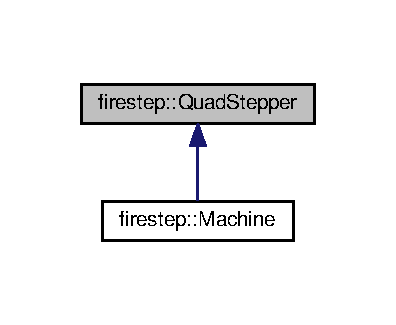
\includegraphics[width=190pt]{classfirestep_1_1_quad_stepper__inherit__graph}
\end{center}
\end{figure}
\subsection*{Public Member Functions}
\begin{DoxyCompactItemize}
\item 
\hypertarget{classfirestep_1_1_quad_stepper_a47fa70b513f25cec74dc14edceef9dca}{virtual Status {\bfseries step} (const \hyperlink{classfirestep_1_1_quad}{Quad}$<$ Step\+D\+V $>$ \&pulse)=0}\label{classfirestep_1_1_quad_stepper_a47fa70b513f25cec74dc14edceef9dca}

\item 
\hypertarget{classfirestep_1_1_quad_stepper_ab77cb4b78de276559e8a0eba8fc1ed7d}{virtual Status {\bfseries step\+Direction} (const \hyperlink{classfirestep_1_1_quad}{Quad}$<$ Step\+D\+V $>$ \&pulse)=0}\label{classfirestep_1_1_quad_stepper_ab77cb4b78de276559e8a0eba8fc1ed7d}

\item 
\hypertarget{classfirestep_1_1_quad_stepper_af4305a3a52466725955de14b196094e2}{virtual Status {\bfseries step\+Fast} (\hyperlink{classfirestep_1_1_quad}{Quad}$<$ Step\+D\+V $>$ \&pulse)=0}\label{classfirestep_1_1_quad_stepper_af4305a3a52466725955de14b196094e2}

\end{DoxyCompactItemize}


The documentation for this class was generated from the following file\+:\begin{DoxyCompactItemize}
\item 
Stroke.\+h\end{DoxyCompactItemize}

\hypertarget{classfirestep_1_1_raw_controller}{\section{firestep\+:\+:Raw\+Controller Class Reference}
\label{classfirestep_1_1_raw_controller}\index{firestep\+::\+Raw\+Controller@{firestep\+::\+Raw\+Controller}}
}


Inheritance diagram for firestep\+:\+:Raw\+Controller\+:
\nopagebreak
\begin{figure}[H]
\begin{center}
\leavevmode
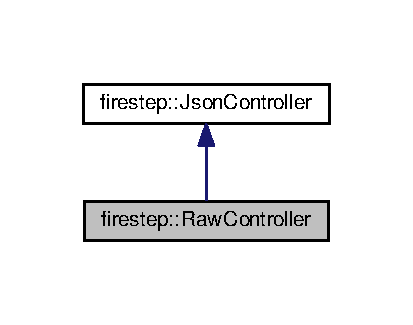
\includegraphics[width=198pt]{classfirestep_1_1_raw_controller__inherit__graph}
\end{center}
\end{figure}


Collaboration diagram for firestep\+:\+:Raw\+Controller\+:
\nopagebreak
\begin{figure}[H]
\begin{center}
\leavevmode
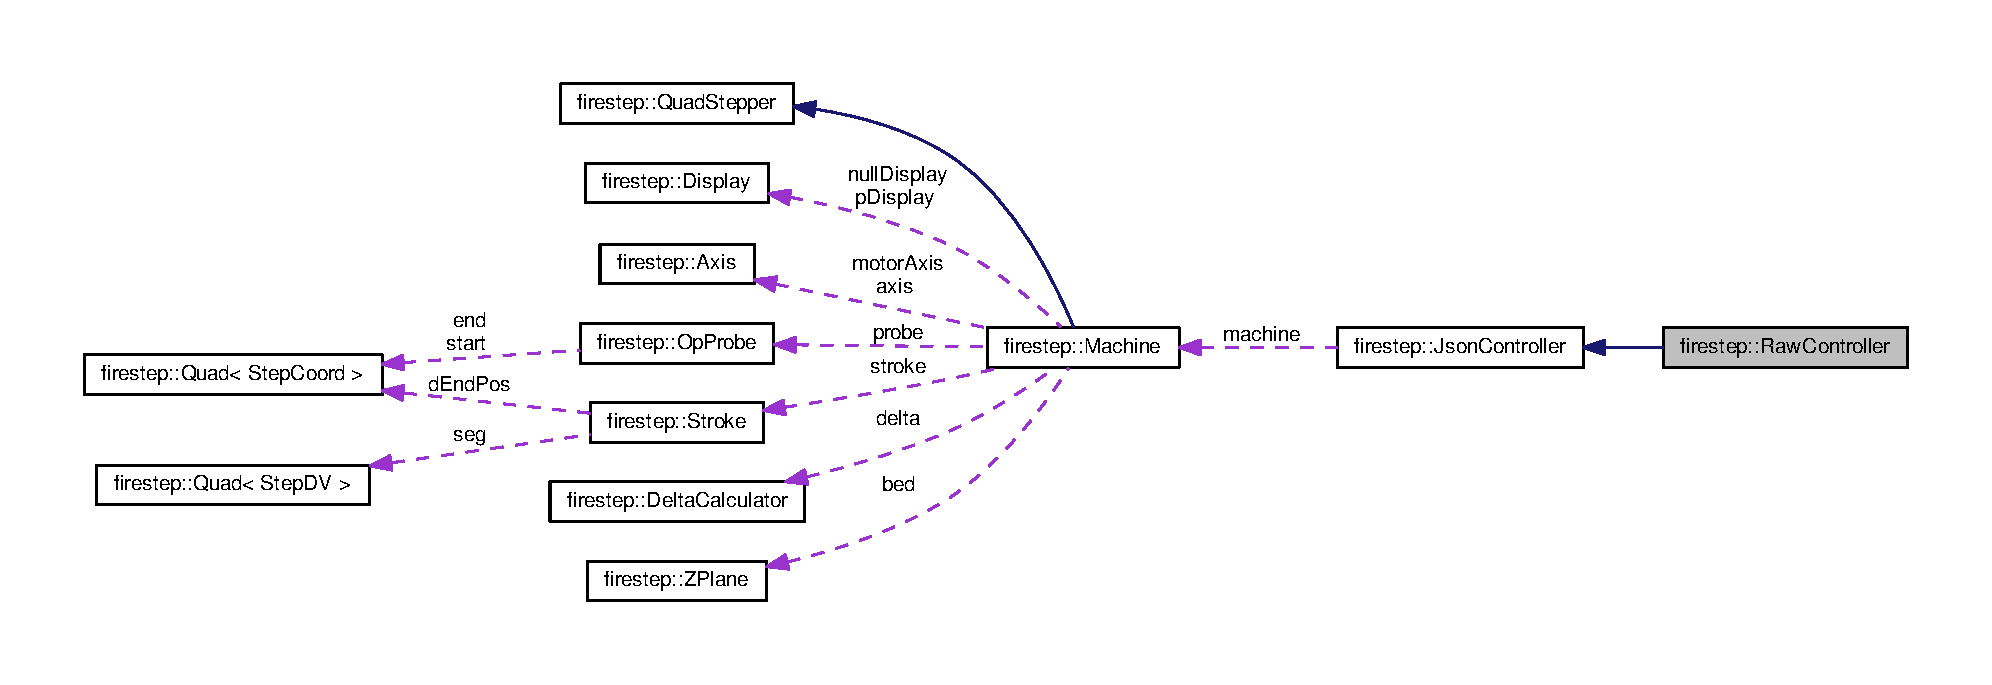
\includegraphics[width=350pt]{classfirestep_1_1_raw_controller__coll__graph}
\end{center}
\end{figure}
\subsection*{Public Member Functions}
\begin{DoxyCompactItemize}
\item 
\hypertarget{classfirestep_1_1_raw_controller_a293df6216a42933432d54bebbb8af801}{{\bfseries Raw\+Controller} (\hyperlink{classfirestep_1_1_machine}{Machine} \&machine)}\label{classfirestep_1_1_raw_controller_a293df6216a42933432d54bebbb8af801}

\item 
\hypertarget{classfirestep_1_1_raw_controller_a47928dcc5b8f8f15ade9803afa6e7e5e}{virtual const char $\ast$ {\bfseries name} ()}\label{classfirestep_1_1_raw_controller_a47928dcc5b8f8f15ade9803afa6e7e5e}

\item 
\hypertarget{classfirestep_1_1_raw_controller_a9c2f0815a53c189eadef1e7d7b701a01}{virtual Status {\bfseries process\+Home} (\hyperlink{classfirestep_1_1_json_command}{Json\+Command} \&jcmd, Json\+Object \&jobj, const char $\ast$key)}\label{classfirestep_1_1_raw_controller_a9c2f0815a53c189eadef1e7d7b701a01}

\item 
\hypertarget{classfirestep_1_1_raw_controller_a964f04820190682fe19bdfe537f95d1d}{virtual Status {\bfseries process\+Move} (\hyperlink{classfirestep_1_1_json_command}{Json\+Command} \&jcmd, Json\+Object \&jobj, const char $\ast$key)}\label{classfirestep_1_1_raw_controller_a964f04820190682fe19bdfe537f95d1d}

\item 
\hypertarget{classfirestep_1_1_raw_controller_aab2d0ed73fda85c29dd29145a04b2642}{virtual Status {\bfseries process\+Probe} (\hyperlink{classfirestep_1_1_json_command}{Json\+Command} \&jcmd, Json\+Object \&jobj, const char $\ast$key)}\label{classfirestep_1_1_raw_controller_aab2d0ed73fda85c29dd29145a04b2642}

\item 
\hypertarget{classfirestep_1_1_raw_controller_ae80c97767a50bdf01c358b30a9a14e5f}{virtual Status {\bfseries process\+Position} (\hyperlink{classfirestep_1_1_json_command}{Json\+Command} \&jcmd, Json\+Object \&jobj, const char $\ast$key)}\label{classfirestep_1_1_raw_controller_ae80c97767a50bdf01c358b30a9a14e5f}

\item 
\hypertarget{classfirestep_1_1_raw_controller_a12d9b40ef8c8a4293c4918bad8c6862c}{virtual Status {\bfseries process\+Dimension} (\hyperlink{classfirestep_1_1_json_command}{Json\+Command} \&jcmd, Json\+Object \&jobj, const char $\ast$key)}\label{classfirestep_1_1_raw_controller_a12d9b40ef8c8a4293c4918bad8c6862c}

\end{DoxyCompactItemize}
\subsection*{Additional Inherited Members}


The documentation for this class was generated from the following files\+:\begin{DoxyCompactItemize}
\item 
Raw\+Controller.\+h\item 
Raw\+Controller.\+cpp\end{DoxyCompactItemize}

\hypertarget{classfirestep_1_1_step3_d}{\section{firestep\+:\+:Step3\+D Class Reference}
\label{classfirestep_1_1_step3_d}\index{firestep\+::\+Step3\+D@{firestep\+::\+Step3\+D}}
}
\subsection*{Public Member Functions}
\begin{DoxyCompactItemize}
\item 
\hypertarget{classfirestep_1_1_step3_d_a71a9267b8090cfd3be24eac48cbd72c1}{{\bfseries Step3\+D} (Step\+Coord p1, Step\+Coord p2, Step\+Coord p3)}\label{classfirestep_1_1_step3_d_a71a9267b8090cfd3be24eac48cbd72c1}

\item 
\hypertarget{classfirestep_1_1_step3_d_abb6f8e9b005c6af8271932d4900a3f0d}{{\bfseries Step3\+D} (bool valid=true, P\+H5\+T\+Y\+P\+E v=0)}\label{classfirestep_1_1_step3_d_abb6f8e9b005c6af8271932d4900a3f0d}

\item 
\hypertarget{classfirestep_1_1_step3_d_a6e926d3e20c3346bafebe9256c7e7337}{bool {\bfseries is\+Valid} ()}\label{classfirestep_1_1_step3_d_a6e926d3e20c3346bafebe9256c7e7337}

\end{DoxyCompactItemize}
\subsection*{Public Attributes}
\begin{DoxyCompactItemize}
\item 
\hypertarget{classfirestep_1_1_step3_d_aac4c0122b81ece8098628efd4e27f51e}{Step\+Coord {\bfseries p1}}\label{classfirestep_1_1_step3_d_aac4c0122b81ece8098628efd4e27f51e}

\item 
\hypertarget{classfirestep_1_1_step3_d_a7276a68e8df0e465524f5a0042c993b4}{Step\+Coord {\bfseries p2}}\label{classfirestep_1_1_step3_d_a7276a68e8df0e465524f5a0042c993b4}

\item 
\hypertarget{classfirestep_1_1_step3_d_aaba7eeabe390843f766607ffb3be067a}{Step\+Coord {\bfseries p3}}\label{classfirestep_1_1_step3_d_aaba7eeabe390843f766607ffb3be067a}

\end{DoxyCompactItemize}


The documentation for this class was generated from the following file\+:\begin{DoxyCompactItemize}
\item 
Delta\+Calculator.\+h\end{DoxyCompactItemize}

\hypertarget{classfirestep_1_1_stroke}{\section{firestep\+:\+:Stroke Class Reference}
\label{classfirestep_1_1_stroke}\index{firestep\+::\+Stroke@{firestep\+::\+Stroke}}
}


Collaboration diagram for firestep\+:\+:Stroke\+:\nopagebreak
\begin{figure}[H]
\begin{center}
\leavevmode
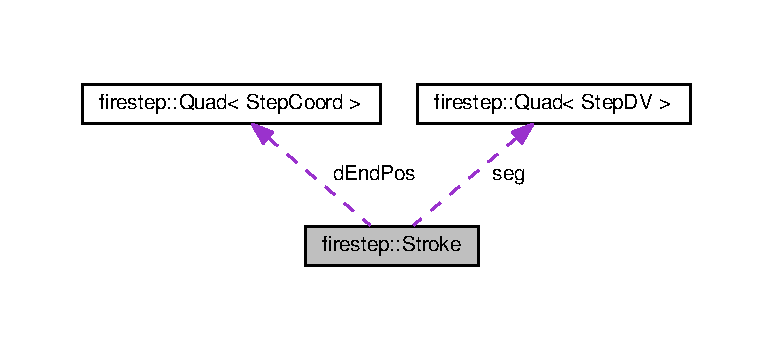
\includegraphics[width=350pt]{classfirestep_1_1_stroke__coll__graph}
\end{center}
\end{figure}
\subsection*{Public Member Functions}
\begin{DoxyCompactItemize}
\item 
\hypertarget{classfirestep_1_1_stroke_a12294d036abe4ae3139d595657afcb06}{void {\bfseries clear} ()}\label{classfirestep_1_1_stroke_a12294d036abe4ae3139d595657afcb06}

\item 
\hypertarget{classfirestep_1_1_stroke_ae9e2089a39ba9c71074f8bf4bfeef07a}{Status {\bfseries start} (Ticks t\+Start)}\label{classfirestep_1_1_stroke_ae9e2089a39ba9c71074f8bf4bfeef07a}

\item 
\hypertarget{classfirestep_1_1_stroke_a9c59dbd44a6a8a1ed0e68a4ed33eaed4}{Status {\bfseries traverse} (Ticks t\+Current, \hyperlink{classfirestep_1_1_quad_stepper}{Quad\+Stepper} \&quad\+Step)}\label{classfirestep_1_1_stroke_a9c59dbd44a6a8a1ed0e68a4ed33eaed4}

\item 
\hypertarget{classfirestep_1_1_stroke_aecf277d0443b4bf91f01889389cbaa59}{bool {\bfseries is\+Done} ()}\label{classfirestep_1_1_stroke_aecf277d0443b4bf91f01889389cbaa59}

\item 
\hypertarget{classfirestep_1_1_stroke_a9c968ddcdbf730ea88c48f7da5aa3197}{\hyperlink{classfirestep_1_1_quad}{Quad}$<$ Step\+Coord $>$ {\bfseries goal\+Pos} (Ticks t)}\label{classfirestep_1_1_stroke_a9c968ddcdbf730ea88c48f7da5aa3197}

\item 
\hypertarget{classfirestep_1_1_stroke_ab08c024119e225fd8b216e849260c90a}{Ticks {\bfseries goal\+Start\+Ticks} (Ticks t)}\label{classfirestep_1_1_stroke_ab08c024119e225fd8b216e849260c90a}

\item 
\hypertarget{classfirestep_1_1_stroke_ab0d238e9d9c06370275f5b6d145d7b92}{Ticks {\bfseries goal\+End\+Ticks} (Ticks t)}\label{classfirestep_1_1_stroke_ab0d238e9d9c06370275f5b6d145d7b92}

\item 
\hypertarget{classfirestep_1_1_stroke_a5c2e64edcac39b1c909a38299d01e668}{Seg\+Index {\bfseries goal\+Segment} (Ticks t)}\label{classfirestep_1_1_stroke_a5c2e64edcac39b1c909a38299d01e668}

\item 
\hypertarget{classfirestep_1_1_stroke_a52c1c232d148553b16832a107fad0ffe}{int16\+\_\+t {\bfseries append} (\hyperlink{classfirestep_1_1_quad}{Quad}$<$ Step\+D\+V $>$ dv)}\label{classfirestep_1_1_stroke_a52c1c232d148553b16832a107fad0ffe}

\item 
\hypertarget{classfirestep_1_1_stroke_a2bf6a591df349d2c424f7e46ff961ea5}{\hyperlink{classfirestep_1_1_quad}{Quad}$<$ Step\+Coord $>$ \& {\bfseries position} ()}\label{classfirestep_1_1_stroke_a2bf6a591df349d2c424f7e46ff961ea5}

\item 
\hypertarget{classfirestep_1_1_stroke_ac5365197d39cdc91dc9fc29e91da7e67}{Ticks {\bfseries get\+\_\+dt\+Total} ()}\label{classfirestep_1_1_stroke_ac5365197d39cdc91dc9fc29e91da7e67}

\item 
\hypertarget{classfirestep_1_1_stroke_a26f9ed72f5cd50357714264652e05f46}{float {\bfseries get\+Time\+Planned} ()}\label{classfirestep_1_1_stroke_a26f9ed72f5cd50357714264652e05f46}

\item 
\hypertarget{classfirestep_1_1_stroke_a7de2d1acd2d2655e22c865d9cc22c4c0}{Ticks {\bfseries get\+Total\+Ticks} ()}\label{classfirestep_1_1_stroke_a7de2d1acd2d2655e22c865d9cc22c4c0}

\item 
\hypertarget{classfirestep_1_1_stroke_a66831fbe6f4670ea0a6d8040ee53b837}{void {\bfseries set\+Time\+Planned} (float seconds)}\label{classfirestep_1_1_stroke_a66831fbe6f4670ea0a6d8040ee53b837}

\end{DoxyCompactItemize}
\subsection*{Public Attributes}
\begin{DoxyCompactItemize}
\item 
\hypertarget{classfirestep_1_1_stroke_a6717b5312700a32011c50912c29c058d}{Ticks {\bfseries t\+Start}}\label{classfirestep_1_1_stroke_a6717b5312700a32011c50912c29c058d}

\item 
\hypertarget{classfirestep_1_1_stroke_af273db9ee21139613c9af959202023bb}{int32\+\_\+t {\bfseries v\+Peak}}\label{classfirestep_1_1_stroke_af273db9ee21139613c9af959202023bb}

\item 
\hypertarget{classfirestep_1_1_stroke_a289c5c1e012d347f77b6359786e646ad}{Step\+Coord {\bfseries scale}}\label{classfirestep_1_1_stroke_a289c5c1e012d347f77b6359786e646ad}

\item 
\hypertarget{classfirestep_1_1_stroke_a1d00ba6a62370fdda82fcc4e5e941c08}{Seg\+Index {\bfseries cur\+Seg}}\label{classfirestep_1_1_stroke_a1d00ba6a62370fdda82fcc4e5e941c08}

\item 
\hypertarget{classfirestep_1_1_stroke_af7b85d7a9d6be39ea78f299b7a15da3a}{Seg\+Index {\bfseries length}}\label{classfirestep_1_1_stroke_af7b85d7a9d6be39ea78f299b7a15da3a}

\item 
\hypertarget{classfirestep_1_1_stroke_a0df9212c33956be8be25c4810d817720}{\hyperlink{classfirestep_1_1_quad}{Quad}$<$ Step\+D\+V $>$ {\bfseries seg} \mbox{[}S\+T\+R\+O\+K\+E\+\_\+\+S\+E\+G\+M\+E\+N\+T\+S\mbox{]}}\label{classfirestep_1_1_stroke_a0df9212c33956be8be25c4810d817720}

\item 
\hypertarget{classfirestep_1_1_stroke_aa189def3d15a829cf2de500dfc753de5}{\hyperlink{classfirestep_1_1_quad}{Quad}$<$ Step\+Coord $>$ {\bfseries d\+End\+Pos}}\label{classfirestep_1_1_stroke_aa189def3d15a829cf2de500dfc753de5}

\end{DoxyCompactItemize}
\subsection*{Friends}
\begin{DoxyCompactItemize}
\item 
\hypertarget{classfirestep_1_1_stroke_a13ac7d286c50427a8e60089ab16eb054}{class {\bfseries Stroke\+Builder}}\label{classfirestep_1_1_stroke_a13ac7d286c50427a8e60089ab16eb054}

\end{DoxyCompactItemize}


The documentation for this class was generated from the following files\+:\begin{DoxyCompactItemize}
\item 
Stroke.\+h\item 
Stroke.\+cpp\end{DoxyCompactItemize}

\hypertarget{classfirestep_1_1_stroke_builder}{\section{firestep\+:\+:Stroke\+Builder Class Reference}
\label{classfirestep_1_1_stroke_builder}\index{firestep\+::\+Stroke\+Builder@{firestep\+::\+Stroke\+Builder}}
}
\subsection*{Public Member Functions}
\begin{DoxyCompactItemize}
\item 
\hypertarget{classfirestep_1_1_stroke_builder_acf6d9a65cacf66f5570485866e9c98a7}{{\bfseries Stroke\+Builder} (int32\+\_\+t v\+Max=12800, float v\+Max\+Seconds=0.\+5, int16\+\_\+t min\+Segments=0, int16\+\_\+t max\+Segments=0)}\label{classfirestep_1_1_stroke_builder_acf6d9a65cacf66f5570485866e9c98a7}

\item 
Status \hyperlink{classfirestep_1_1_stroke_builder_a24e49b2f3dce062201bffc50e387179f}{build\+Line} (\hyperlink{classfirestep_1_1_stroke}{Stroke} \&stroke, \hyperlink{classfirestep_1_1_quad}{Quad}$<$ Step\+Coord $>$ d\+Pos)
\end{DoxyCompactItemize}
\subsection*{Public Attributes}
\begin{DoxyCompactItemize}
\item 
\hypertarget{classfirestep_1_1_stroke_builder_adf2373e742a16c7c8b2d6d483d0770e6}{int32\+\_\+t {\bfseries v\+Max}}\label{classfirestep_1_1_stroke_builder_adf2373e742a16c7c8b2d6d483d0770e6}

\item 
\hypertarget{classfirestep_1_1_stroke_builder_abe594e40d2d7880cc54c7a52a1f1dd4f}{float {\bfseries v\+Max\+Seconds}}\label{classfirestep_1_1_stroke_builder_abe594e40d2d7880cc54c7a52a1f1dd4f}

\item 
\hypertarget{classfirestep_1_1_stroke_builder_ad6ba092a82a1f2e51454d534fe7a9a57}{int16\+\_\+t {\bfseries min\+Segments}}\label{classfirestep_1_1_stroke_builder_ad6ba092a82a1f2e51454d534fe7a9a57}

\item 
\hypertarget{classfirestep_1_1_stroke_builder_afda030dbed4139af1ec75f43c4c5efa4}{int16\+\_\+t {\bfseries max\+Segments}}\label{classfirestep_1_1_stroke_builder_afda030dbed4139af1ec75f43c4c5efa4}

\end{DoxyCompactItemize}


\subsection{Member Function Documentation}
\hypertarget{classfirestep_1_1_stroke_builder_a24e49b2f3dce062201bffc50e387179f}{\index{firestep\+::\+Stroke\+Builder@{firestep\+::\+Stroke\+Builder}!build\+Line@{build\+Line}}
\index{build\+Line@{build\+Line}!firestep\+::\+Stroke\+Builder@{firestep\+::\+Stroke\+Builder}}
\subsubsection[{build\+Line}]{\setlength{\rightskip}{0pt plus 5cm}Status Stroke\+Builder\+::build\+Line (
\begin{DoxyParamCaption}
\item[{{\bf Stroke} \&}]{stroke, }
\item[{{\bf Quad}$<$ Step\+Coord $>$}]{rel\+Pos}
\end{DoxyParamCaption}
)}}\label{classfirestep_1_1_stroke_builder_a24e49b2f3dce062201bffc50e387179f}
Create a line by scaling a known P\+H5\+Curve to match the requested linear offset. 

The documentation for this class was generated from the following files\+:\begin{DoxyCompactItemize}
\item 
Stroke.\+h\item 
Stroke.\+cpp\end{DoxyCompactItemize}

\hypertarget{structfirestep_1_1_thread}{\section{firestep\+:\+:Thread Struct Reference}
\label{structfirestep_1_1_thread}\index{firestep\+::\+Thread@{firestep\+::\+Thread}}
}


Inheritance diagram for firestep\+:\+:Thread\+:
\nopagebreak
\begin{figure}[H]
\begin{center}
\leavevmode
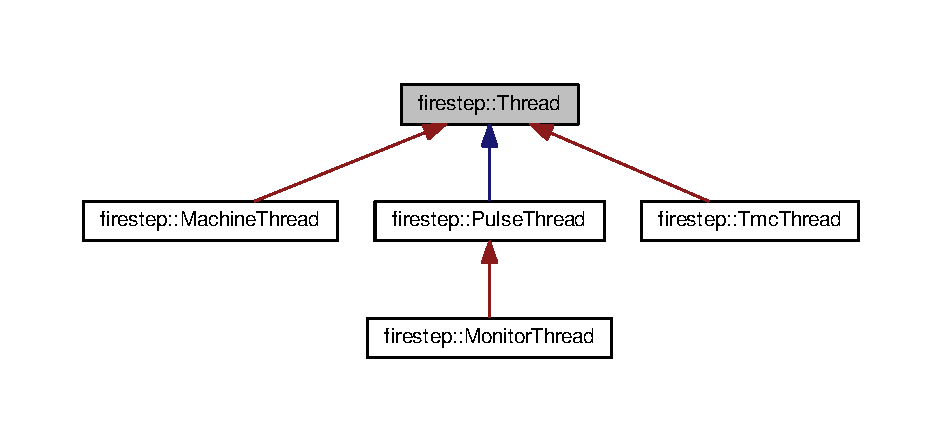
\includegraphics[width=350pt]{structfirestep_1_1_thread__inherit__graph}
\end{center}
\end{figure}


Collaboration diagram for firestep\+:\+:Thread\+:\nopagebreak
\begin{figure}[H]
\begin{center}
\leavevmode
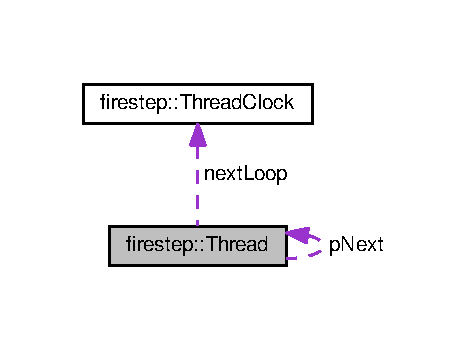
\includegraphics[width=225pt]{structfirestep_1_1_thread__coll__graph}
\end{center}
\end{figure}
\subsection*{Public Member Functions}
\begin{DoxyCompactItemize}
\item 
\hypertarget{structfirestep_1_1_thread_ac38e34ed047af769da29d3ea0de7a9af}{virtual void {\bfseries setup} ()}\label{structfirestep_1_1_thread_ac38e34ed047af769da29d3ea0de7a9af}

\item 
\hypertarget{structfirestep_1_1_thread_a1d0bdb9bf79a9ccb654d7cad0cbae0d8}{virtual void {\bfseries loop} ()}\label{structfirestep_1_1_thread_a1d0bdb9bf79a9ccb654d7cad0cbae0d8}

\end{DoxyCompactItemize}
\subsection*{Public Attributes}
\begin{DoxyCompactItemize}
\item 
\hypertarget{structfirestep_1_1_thread_aa8b92a83425f701377f1bd043c8d2c2e}{struct \hyperlink{structfirestep_1_1_thread}{Thread} $\ast$ {\bfseries p\+Next}}\label{structfirestep_1_1_thread_aa8b92a83425f701377f1bd043c8d2c2e}

\item 
\hypertarget{structfirestep_1_1_thread_a6454f4d8c71fdfed974294d9ed67c4b7}{\hyperlink{unionfirestep_1_1_thread_clock}{Thread\+Clock} {\bfseries next\+Loop}}\label{structfirestep_1_1_thread_a6454f4d8c71fdfed974294d9ed67c4b7}

\item 
\hypertarget{structfirestep_1_1_thread_a1374fd754ad90ed5085d9a8e594a12cf}{byte {\bfseries tardies}}\label{structfirestep_1_1_thread_a1374fd754ad90ed5085d9a8e594a12cf}

\item 
\hypertarget{structfirestep_1_1_thread_aea421383327277a6975fc5893b747eca}{char {\bfseries id}}\label{structfirestep_1_1_thread_aea421383327277a6975fc5893b747eca}

\end{DoxyCompactItemize}


The documentation for this struct was generated from the following files\+:\begin{DoxyCompactItemize}
\item 
Thread.\+h\item 
Thread.\+cpp\end{DoxyCompactItemize}

\hypertarget{unionfirestep_1_1_thread_clock}{\section{firestep\+:\+:Thread\+Clock Union Reference}
\label{unionfirestep_1_1_thread_clock}\index{firestep\+::\+Thread\+Clock@{firestep\+::\+Thread\+Clock}}
}
\subsection*{Public Attributes}
\begin{DoxyCompactItemize}
\item 
\hypertarget{unionfirestep_1_1_thread_clock_a859aa303c5837ab9668a037074b34fb6}{Ticks {\bfseries ticks}}\label{unionfirestep_1_1_thread_clock_a859aa303c5837ab9668a037074b34fb6}

\item 
\hypertarget{unionfirestep_1_1_thread_clock_a58c5f0241a955124ce4ff137eaa2bd23}{\begin{tabbing}
xx\=xx\=xx\=xx\=xx\=xx\=xx\=xx\=xx\=\kill
struct \{\\
\hypertarget{structfirestep_1_1_thread_clock_1_1@1_a06204218df309aa4e9b42d6dc5da3b87}{\>uint16\_t {\bfseries age}\\
\hypertarget{structfirestep_1_1_thread_clock_1_1@1_a9961481b03c07193c4587fbdbf3dbe61}{\>uint16\_t {\bfseries generation}\\
\}; }\label{unionfirestep_1_1_thread_clock_a58c5f0241a955124ce4ff137eaa2bd23}
\\

\end{tabbing}\end{DoxyCompactItemize}


The documentation for this union was generated from the following file\+:\begin{DoxyCompactItemize}
\item 
Thread.\+h\end{DoxyCompactItemize}

\hypertarget{classfirestep_1_1_thread_runner}{\section{firestep\+:\+:Thread\+Runner Class Reference}
\label{classfirestep_1_1_thread_runner}\index{firestep\+::\+Thread\+Runner@{firestep\+::\+Thread\+Runner}}
}
\subsection*{Public Member Functions}
\begin{DoxyCompactItemize}
\item 
void \hyperlink{classfirestep_1_1_thread_runner_a5d0618373b9fb949f04ae923af314842}{reset\+Generations} ()
\item 
\hypertarget{classfirestep_1_1_thread_runner_a98c086925b952cff676e6709410ab7c5}{void {\bfseries clear} ()}\label{classfirestep_1_1_thread_runner_a98c086925b952cff676e6709410ab7c5}

\item 
\hypertarget{classfirestep_1_1_thread_runner_a510ecff046fe75f5e59a8785e627fc78}{void {\bfseries setup} (int pin\+L\+E\+D=N\+O\+P\+I\+N)}\label{classfirestep_1_1_thread_runner_a510ecff046fe75f5e59a8785e627fc78}

\item 
\hypertarget{classfirestep_1_1_thread_runner_a8a04d5dcf14c421898c15d4131dfd76c}{void {\bfseries run} ()}\label{classfirestep_1_1_thread_runner_a8a04d5dcf14c421898c15d4131dfd76c}

\item 
\hypertarget{classfirestep_1_1_thread_runner_ae4da2c930a006078a3450015083c937f}{uint16\+\_\+t {\bfseries get\+\_\+generation} ()}\label{classfirestep_1_1_thread_runner_ae4da2c930a006078a3450015083c937f}

\item 
\hypertarget{classfirestep_1_1_thread_runner_a94b41f44713663aec974d2e0265bf37f}{uint16\+\_\+t {\bfseries get\+\_\+last\+Age} ()}\label{classfirestep_1_1_thread_runner_a94b41f44713663aec974d2e0265bf37f}

\item 
\hypertarget{classfirestep_1_1_thread_runner_af6d87e51d9bb2e8c8f41ee5ad1cda433}{uint16\+\_\+t {\bfseries get\+\_\+age} ()}\label{classfirestep_1_1_thread_runner_af6d87e51d9bb2e8c8f41ee5ad1cda433}

\item 
\hypertarget{classfirestep_1_1_thread_runner_acb58f24aac14aebc3cc5142e3a0dbd0a}{byte {\bfseries get\+\_\+test\+Tardies} ()}\label{classfirestep_1_1_thread_runner_acb58f24aac14aebc3cc5142e3a0dbd0a}

\item 
\hypertarget{classfirestep_1_1_thread_runner_a81dcee95d66b4f5b55cadeae7c8a4c0c}{void {\bfseries outer\+Loop} ()}\label{classfirestep_1_1_thread_runner_a81dcee95d66b4f5b55cadeae7c8a4c0c}

\item 
\hypertarget{classfirestep_1_1_thread_runner_af525cf4560839eaf8f7fce9bab130753}{Ticks {\bfseries ticks} ()}\label{classfirestep_1_1_thread_runner_af525cf4560839eaf8f7fce9bab130753}

\item 
\hypertarget{classfirestep_1_1_thread_runner_ab9089243b03441fb9c232baf517ec5b1}{byte {\bfseries inner\+Loop} ()}\label{classfirestep_1_1_thread_runner_ab9089243b03441fb9c232baf517ec5b1}

\end{DoxyCompactItemize}


\subsection{Member Function Documentation}
\hypertarget{classfirestep_1_1_thread_runner_a5d0618373b9fb949f04ae923af314842}{\index{firestep\+::\+Thread\+Runner@{firestep\+::\+Thread\+Runner}!reset\+Generations@{reset\+Generations}}
\index{reset\+Generations@{reset\+Generations}!firestep\+::\+Thread\+Runner@{firestep\+::\+Thread\+Runner}}
\subsubsection[{reset\+Generations}]{\setlength{\rightskip}{0pt plus 5cm}void Thread\+Runner\+::reset\+Generations (
\begin{DoxyParamCaption}
{}
\end{DoxyParamCaption}
)}}\label{classfirestep_1_1_thread_runner_a5d0618373b9fb949f04ae923af314842}
The generation count has exceeded the maximum. Give the machine a rest and power-\/cycle it. 

The documentation for this class was generated from the following files\+:\begin{DoxyCompactItemize}
\item 
Thread.\+h\item 
Thread.\+cpp\end{DoxyCompactItemize}

\hypertarget{classfirestep_1_1_tmc_thread}{\section{firestep\+:\+:Tmc\+Thread Class Reference}
\label{classfirestep_1_1_tmc_thread}\index{firestep\+::\+Tmc\+Thread@{firestep\+::\+Tmc\+Thread}}
}


Inheritance diagram for firestep\+:\+:Tmc\+Thread\+:
\nopagebreak
\begin{figure}[H]
\begin{center}
\leavevmode
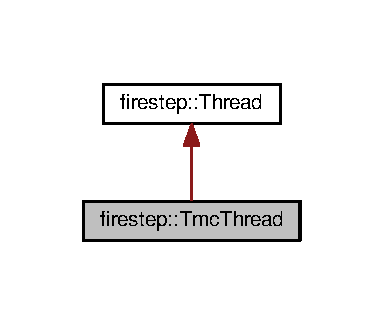
\includegraphics[width=184pt]{classfirestep_1_1_tmc_thread__inherit__graph}
\end{center}
\end{figure}


Collaboration diagram for firestep\+:\+:Tmc\+Thread\+:
\nopagebreak
\begin{figure}[H]
\begin{center}
\leavevmode
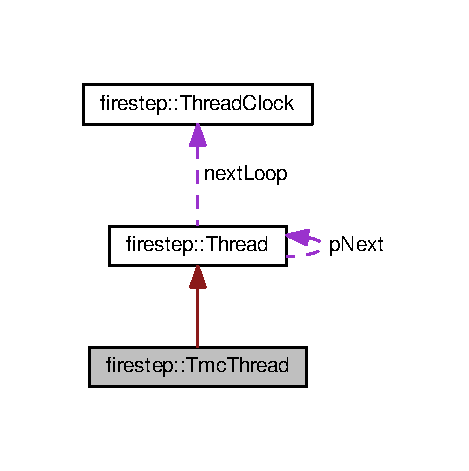
\includegraphics[width=225pt]{classfirestep_1_1_tmc_thread__coll__graph}
\end{center}
\end{figure}
\subsection*{Public Member Functions}
\begin{DoxyCompactItemize}
\item 
\hypertarget{classfirestep_1_1_tmc_thread_aa6f36b40da306eb2d9050ceae13b432f}{void {\bfseries setup} ()}\label{classfirestep_1_1_tmc_thread_aa6f36b40da306eb2d9050ceae13b432f}

\item 
\hypertarget{classfirestep_1_1_tmc_thread_a6036f09286e1429ec41bbb04b86f7c21}{void {\bfseries loop} ()}\label{classfirestep_1_1_tmc_thread_a6036f09286e1429ec41bbb04b86f7c21}

\end{DoxyCompactItemize}
\subsection*{Public Attributes}
\begin{DoxyCompactItemize}
\item 
\hypertarget{classfirestep_1_1_tmc_thread_acf160b2ffe709639e8caaf8320bf5b00}{uint8\+\_\+t {\bfseries tmc\+Led\+Pin}}\label{classfirestep_1_1_tmc_thread_acf160b2ffe709639e8caaf8320bf5b00}

\item 
\hypertarget{classfirestep_1_1_tmc_thread_ab54cefd6ad811806cde581daf170704b}{uint8\+\_\+t {\bfseries tmc\+Led\+Value}}\label{classfirestep_1_1_tmc_thread_ab54cefd6ad811806cde581daf170704b}

\item 
\hypertarget{classfirestep_1_1_tmc_thread_a6c43133b36e318002ef0d41d35e8ee6c}{uint16\+\_\+t {\bfseries loadmeas}}\label{classfirestep_1_1_tmc_thread_a6c43133b36e318002ef0d41d35e8ee6c}

\item 
\hypertarget{classfirestep_1_1_tmc_thread_a78d09c196ac6ed2464e948a8720a5ead}{uint16\+\_\+t {\bfseries loadmeas\+\_\+max}}\label{classfirestep_1_1_tmc_thread_a78d09c196ac6ed2464e948a8720a5ead}

\item 
\hypertarget{classfirestep_1_1_tmc_thread_a2c1371eb935aeb4c5fce044e17420c45}{uint16\+\_\+t {\bfseries loadmeas\+\_\+min}}\label{classfirestep_1_1_tmc_thread_a2c1371eb935aeb4c5fce044e17420c45}

\item 
\hypertarget{classfirestep_1_1_tmc_thread_a6cc2118ff1e2d38dd0eae127c5dee960}{uint32\+\_\+t {\bfseries tstep}}\label{classfirestep_1_1_tmc_thread_a6cc2118ff1e2d38dd0eae127c5dee960}

\end{DoxyCompactItemize}


The documentation for this class was generated from the following files\+:\begin{DoxyCompactItemize}
\item 
Tmc\+Thread.\+h\item 
Tmc\+Thread.\+cpp\end{DoxyCompactItemize}

\hypertarget{classfirestep_1_1_x_y_z3_d}{\section{firestep\+:\+:X\+Y\+Z3\+D Class Reference}
\label{classfirestep_1_1_x_y_z3_d}\index{firestep\+::\+X\+Y\+Z3\+D@{firestep\+::\+X\+Y\+Z3\+D}}
}
\subsection*{Public Member Functions}
\begin{DoxyCompactItemize}
\item 
\hypertarget{classfirestep_1_1_x_y_z3_d_a19c385a7182555f53ac694d18676fac2}{{\bfseries X\+Y\+Z3\+D} (P\+H5\+T\+Y\+P\+E x, P\+H5\+T\+Y\+P\+E y, P\+H5\+T\+Y\+P\+E z)}\label{classfirestep_1_1_x_y_z3_d_a19c385a7182555f53ac694d18676fac2}

\item 
\hypertarget{classfirestep_1_1_x_y_z3_d_aacbdc08bc3a78c8e6b5b89e3a4dbea32}{{\bfseries X\+Y\+Z3\+D} (bool valid=true, P\+H5\+T\+Y\+P\+E v=0)}\label{classfirestep_1_1_x_y_z3_d_aacbdc08bc3a78c8e6b5b89e3a4dbea32}

\item 
\hypertarget{classfirestep_1_1_x_y_z3_d_ad8519c362062072cd60dc6b99be46fd6}{bool {\bfseries operator==} (const \hyperlink{classfirestep_1_1_x_y_z3_d}{X\+Y\+Z3\+D} \&that)}\label{classfirestep_1_1_x_y_z3_d_ad8519c362062072cd60dc6b99be46fd6}

\item 
\hypertarget{classfirestep_1_1_x_y_z3_d_aa0a31f297a4ff1af505c7bd2e82958cd}{bool {\bfseries operator!=} (const \hyperlink{classfirestep_1_1_x_y_z3_d}{X\+Y\+Z3\+D} \&that)}\label{classfirestep_1_1_x_y_z3_d_aa0a31f297a4ff1af505c7bd2e82958cd}

\item 
\hypertarget{classfirestep_1_1_x_y_z3_d_ac005432a98872b720e8642b75bb78742}{bool {\bfseries is\+Valid} ()}\label{classfirestep_1_1_x_y_z3_d_ac005432a98872b720e8642b75bb78742}

\end{DoxyCompactItemize}
\subsection*{Public Attributes}
\begin{DoxyCompactItemize}
\item 
\hypertarget{classfirestep_1_1_x_y_z3_d_a08d7642966a1c18428bf0373a5b21ce8}{P\+H5\+T\+Y\+P\+E {\bfseries x}}\label{classfirestep_1_1_x_y_z3_d_a08d7642966a1c18428bf0373a5b21ce8}

\item 
\hypertarget{classfirestep_1_1_x_y_z3_d_aa192393e7736301cf1c4357981fbff26}{P\+H5\+T\+Y\+P\+E {\bfseries y}}\label{classfirestep_1_1_x_y_z3_d_aa192393e7736301cf1c4357981fbff26}

\item 
\hypertarget{classfirestep_1_1_x_y_z3_d_a4bbd94171a6b45a71d19f5a38449bdb8}{P\+H5\+T\+Y\+P\+E {\bfseries z}}\label{classfirestep_1_1_x_y_z3_d_a4bbd94171a6b45a71d19f5a38449bdb8}

\end{DoxyCompactItemize}


The documentation for this class was generated from the following file\+:\begin{DoxyCompactItemize}
\item 
Delta\+Calculator.\+h\end{DoxyCompactItemize}

\hypertarget{classfirestep_1_1_z_plane}{\section{firestep\+:\+:Z\+Plane Class Reference}
\label{classfirestep_1_1_z_plane}\index{firestep\+::\+Z\+Plane@{firestep\+::\+Z\+Plane}}
}
\subsection*{Public Member Functions}
\begin{DoxyCompactItemize}
\item 
\hypertarget{classfirestep_1_1_z_plane_a791f0547290a3fa0545a60f75adf0620}{{\bfseries Z\+Plane} (P\+H5\+T\+Y\+P\+E a=0, P\+H5\+T\+Y\+P\+E b=0, P\+H5\+T\+Y\+P\+E c=0)}\label{classfirestep_1_1_z_plane_a791f0547290a3fa0545a60f75adf0620}

\item 
\hypertarget{classfirestep_1_1_z_plane_a29fa12b27615771ce4a451cb2bb4291c}{\hyperlink{classfirestep_1_1_z_plane}{Z\+Plane} \& {\bfseries operator=} (const \hyperlink{classfirestep_1_1_z_plane}{Z\+Plane} that)}\label{classfirestep_1_1_z_plane_a29fa12b27615771ce4a451cb2bb4291c}

\item 
\hypertarget{classfirestep_1_1_z_plane_a1f78df2693f360f78e203029d7347124}{bool {\bfseries initialize} (\hyperlink{classfirestep_1_1_x_y_z3_d}{X\+Y\+Z3\+D} p1, \hyperlink{classfirestep_1_1_x_y_z3_d}{X\+Y\+Z3\+D} p2, \hyperlink{classfirestep_1_1_x_y_z3_d}{X\+Y\+Z3\+D} p3)}\label{classfirestep_1_1_z_plane_a1f78df2693f360f78e203029d7347124}

\item 
\hypertarget{classfirestep_1_1_z_plane_ac7ce8f801cad2ceb839f9ecf17002f9d}{P\+H5\+T\+Y\+P\+E {\bfseries calc\+Z} (P\+H5\+T\+Y\+P\+E x, P\+H5\+T\+Y\+P\+E y)}\label{classfirestep_1_1_z_plane_ac7ce8f801cad2ceb839f9ecf17002f9d}

\item 
\hypertarget{classfirestep_1_1_z_plane_acde7d2b1955a9f921be7618eda425ca8}{P\+H5\+T\+Y\+P\+E {\bfseries get\+X\+Scale} ()}\label{classfirestep_1_1_z_plane_acde7d2b1955a9f921be7618eda425ca8}

\item 
\hypertarget{classfirestep_1_1_z_plane_aa8fc8741e87601bbba9eeb6d1838f14c}{P\+H5\+T\+Y\+P\+E {\bfseries get\+Y\+Scale} ()}\label{classfirestep_1_1_z_plane_aa8fc8741e87601bbba9eeb6d1838f14c}

\item 
\hypertarget{classfirestep_1_1_z_plane_ac4df8b10208e79164acffdf930ffa3f3}{P\+H5\+T\+Y\+P\+E {\bfseries get\+Z\+Offset} ()}\label{classfirestep_1_1_z_plane_ac4df8b10208e79164acffdf930ffa3f3}

\item 
\hypertarget{classfirestep_1_1_z_plane_aed64c33e7a40d0c10544ad225d483c1e}{void {\bfseries set\+Z\+Offset} (P\+H5\+T\+Y\+P\+E value)}\label{classfirestep_1_1_z_plane_aed64c33e7a40d0c10544ad225d483c1e}

\end{DoxyCompactItemize}
\subsection*{Public Attributes}
\begin{DoxyCompactItemize}
\item 
\hypertarget{classfirestep_1_1_z_plane_acbd7fb27fe0c4545f8bd3a55f704faca}{P\+H5\+T\+Y\+P\+E {\bfseries a}}\label{classfirestep_1_1_z_plane_acbd7fb27fe0c4545f8bd3a55f704faca}

\item 
\hypertarget{classfirestep_1_1_z_plane_a0ea810f77f4fdc34fd4242be330cdfef}{P\+H5\+T\+Y\+P\+E {\bfseries b}}\label{classfirestep_1_1_z_plane_a0ea810f77f4fdc34fd4242be330cdfef}

\item 
\hypertarget{classfirestep_1_1_z_plane_a2a18af1a7c62c7113b72fa884750f388}{P\+H5\+T\+Y\+P\+E {\bfseries c}}\label{classfirestep_1_1_z_plane_a2a18af1a7c62c7113b72fa884750f388}

\end{DoxyCompactItemize}


The documentation for this class was generated from the following files\+:\begin{DoxyCompactItemize}
\item 
Machine.\+h\item 
Machine.\+cpp\end{DoxyCompactItemize}

%--- End generated contents ---

% Index
\newpage
\phantomsection
\addcontentsline{toc}{chapter}{Index}
\printindex

\end{document}
